\section{Ecken kompatible Paare}

In diesem Abschnitt werden wir uns mit einer zweiten Charakterisierung von SLTRs auf planaren Graphen nach \cite{af15} beschäftigen, die eine Verbindung zwischen Schnyder Woods und FAAs herstellt und so zu einer hinreichenden Bedingung für SLTRs führt. Zum Einstieg folgt die Definition dieses Zusammenhanges.

\begin{definition}[Ecken Kompatibilität]\label{def_ccc}
Ein Paar $(\sigma,\phi)$ aus einem Schnyder Labeling $\sigma$ und einem FAA $\phi$ nennen wir \textit{Ecken kompatibel}, falls:
\begin{itemize}
\item [K1] Das Schnyder Labeling $\sigma$ und das FAA $\phi$ die selben Aufhängungen nutzen, und
\item [K2] die drei Ecken aus $\phi$ in jedem inneren Gebiet drei unterschiedliche Label in $\sigma$ haben.
\end{itemize}
\end{definition}

\begin{example}
Wir greifen vor und nehmen an, dass ein Graph genau dann eine SLTR zulässt, wenn ein Ecken kompatibles Paar existiert. Wir müssen für die Beantwortung, ob ein Graph eine SLTR zulässt unter Umständen alle Schnyder Woods von $G$ überprüfen. Dies sehen wir anhand von Abbildung \ref{exp_ccc}. Hier ist derselbe Graph mit zwei unterschiedlichen Schnyder Labelings abgebildet. Zu dem Labeling auf der linken Seite existiert ein Ecken kompatibles FAA. Auf der rechten Seite kann kein solches FAA existieren. Wie wir auf der linken Seite sehen, muss jeder innere Knoten zugewiesen werden. Insbesondere also der Knoten $v$. Dann fehlt jedoch im zugewiesenen Gebiet eine Ecke mit diesem Label, da die Label an $v$ jeweils nur einmal in den Gebieten auftreten.

\begin{figure}[h]
\centering
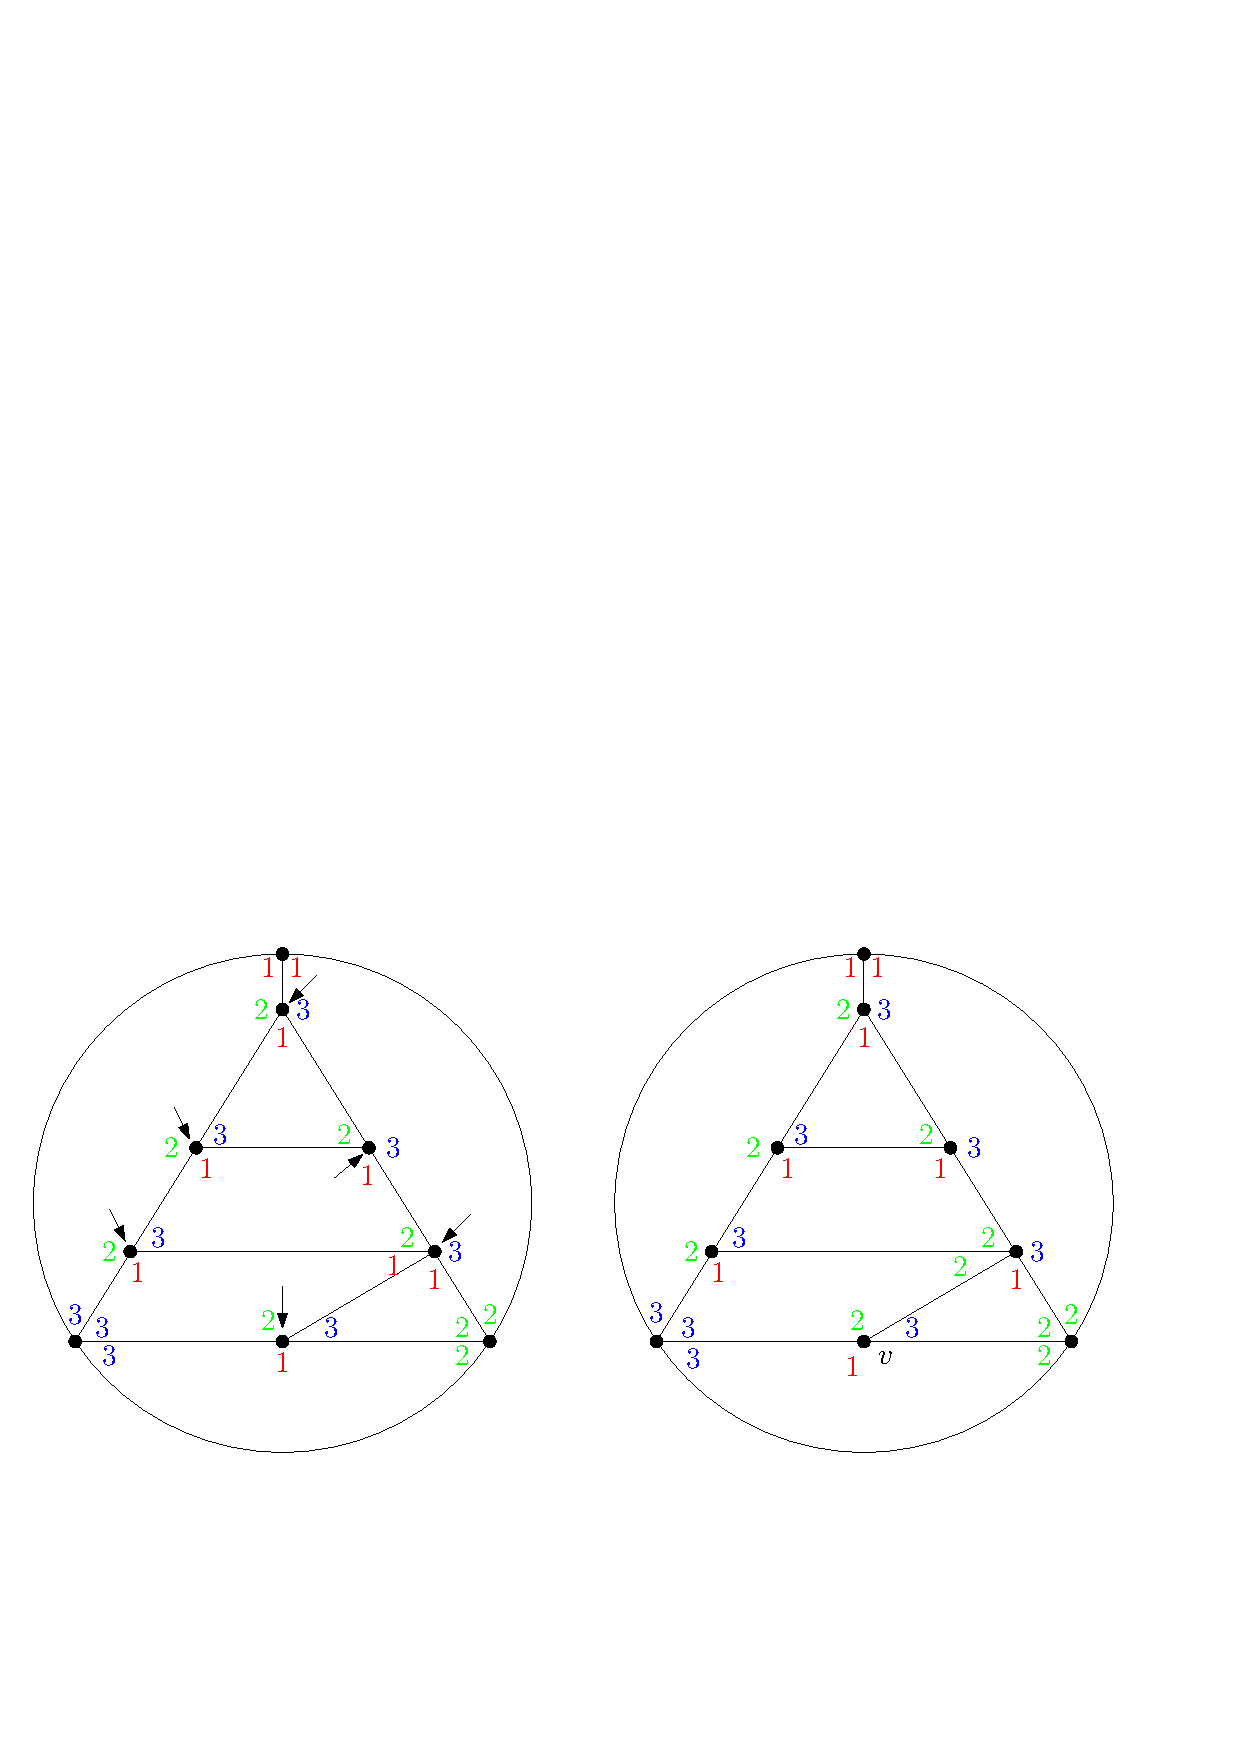
\includegraphics[width=0.9\textwidth]{exp_ccc.pdf}
\caption{Nicht jedes Schnyder Labeling lässt ein Ecken kompatibles Paar zu, selbst wenn der Graph eine SLTR hat.}
\label{exp_ccc}
\end{figure}

\end{example}

Der Rest dieses Kapitels wird sich mit dem Beweis beschäftigen, dass zu jedem SLTR (mindestens) ein Ecken kompatibles Paar existiert, und dass andersherum jedes Ecken kompatible Paar eine SLTR induziert. 

\begin{theorem}\label{theo_ccc}
Sei G ein ebener, intern-3-zusammenhängender Graph mit den Aufhängungen $\{a_1,a_2,a_3\}$. G besitzt genau dann eine SLTR, wenn ein Ecken kompatibles Paar $(\sigma,\phi)$ aus einem Schnyder Labeling $\sigma$ und einem FAA $\phi$ existiert.
\end{theorem}

Wir beweisen zuerst die (deutlich einfachere) Rückrichtung des Theorems. Hier können wir die durch das in Abschnitt \ref{face_counting} erklärte \textit{face-counting} erhaltene Einbettung nutzen, um zu zeigen, dass jeder begrenzende Zykel $\gamma$ mindestens drei kombinatorisch konvexe Ecken besitzt. 

\begin{lemma}\label{lem1}
Sei G ein ebener, intern-3-zusammenhängender Graph mit den Aufhängungen $\{a_1,a_2,a_3\}$. Falls ein Paar $(\sigma,\phi)$ aus einem Schnyder Labeling $\sigma$ und einem FAA $\phi$ Ecken kompatibel ist, dann hat jeder begrenzende Zykel $\gamma$, der nicht von einem Pfad induziert wird, mindestens drei kombinatorisch konvexe Ecken im Bezug auf $\phi$.
\end{lemma}

\begin{proof}
Sei $\gamma$ ein begrenzender Zykel und $F_{in}$ die Menge der inneren Gebiete von $G$. Seien $\alpha_1=(0,1),\alpha_2=(1,0)$ und $\alpha_3=(0,0)$ die Bilder der Aufhängungen und $D$ die durch \textit{face counting} erhaltende Zeichnung von $G$ mit den Ecken $\alpha_1,\alpha_2,\alpha_3$. Ein Beispiel einer solchen Zeichnung findet sich in Abbildung \ref{face_counting}. Betrachte nun den begrenzenden Zykel $\gamma$ in $D$. Wir schieben nun, wie in Abbildung \ref{sweeplines1} illustriert, ausgehend von $\alpha_i$ die Geraden $(\alpha_{i+1},\alpha_{i-1})$ über den Graphen. Sei $M_i$ die Menge der zuerst von $(\alpha_{i+1},\alpha_{i-1})$ getroffenen Knoten von $\gamma$ für $i \in (1,2,3)$.

\begin{observation}\label{obs1}
Alle Knoten um ein inneres Gebiet $f$ mit Label $i$ in $f$ werden von der Gerade $(\alpha_{i+1},\alpha_{i-1})$ zum gleichen Zeitpunkt getroffen. Dies folgt direkt aus Proposition \ref{w5} W5, weil alle Knoten mit dem selben Label in der Zeichnung auf $c_i(\alpha_{i+1},\alpha_{i-1})$ platziert werden.
\end{observation}

\begin{observation}\label{obs2}
Sei $v \in M_i$. Alle Winkel an $v$ im Inneren von $\gamma$ haben das Label $i$. Die Geraden $(\alpha_{i+1},\alpha_{i-1})$ teilen die Winkel um einen Knoten in Intervalle (siehe Abbildung \ref{sweeplines2}). Die Winkel an $v$, die von $a_i$ aus gesehen vollständig auf der anderen Seite der Gerade $(\alpha_{i+1},\alpha_{i-1})$ liegen, haben Label $i$.
\end{observation}

\captionsetup{format=plain,labelsep=endash,justification=raggedright,width=.47\textwidth}

\begin{figure}
\centering
\begin{minipage}{0.2\textwidth}
  \end{minipage}
  \begin{minipage}{0.45\textwidth}
  \centering
    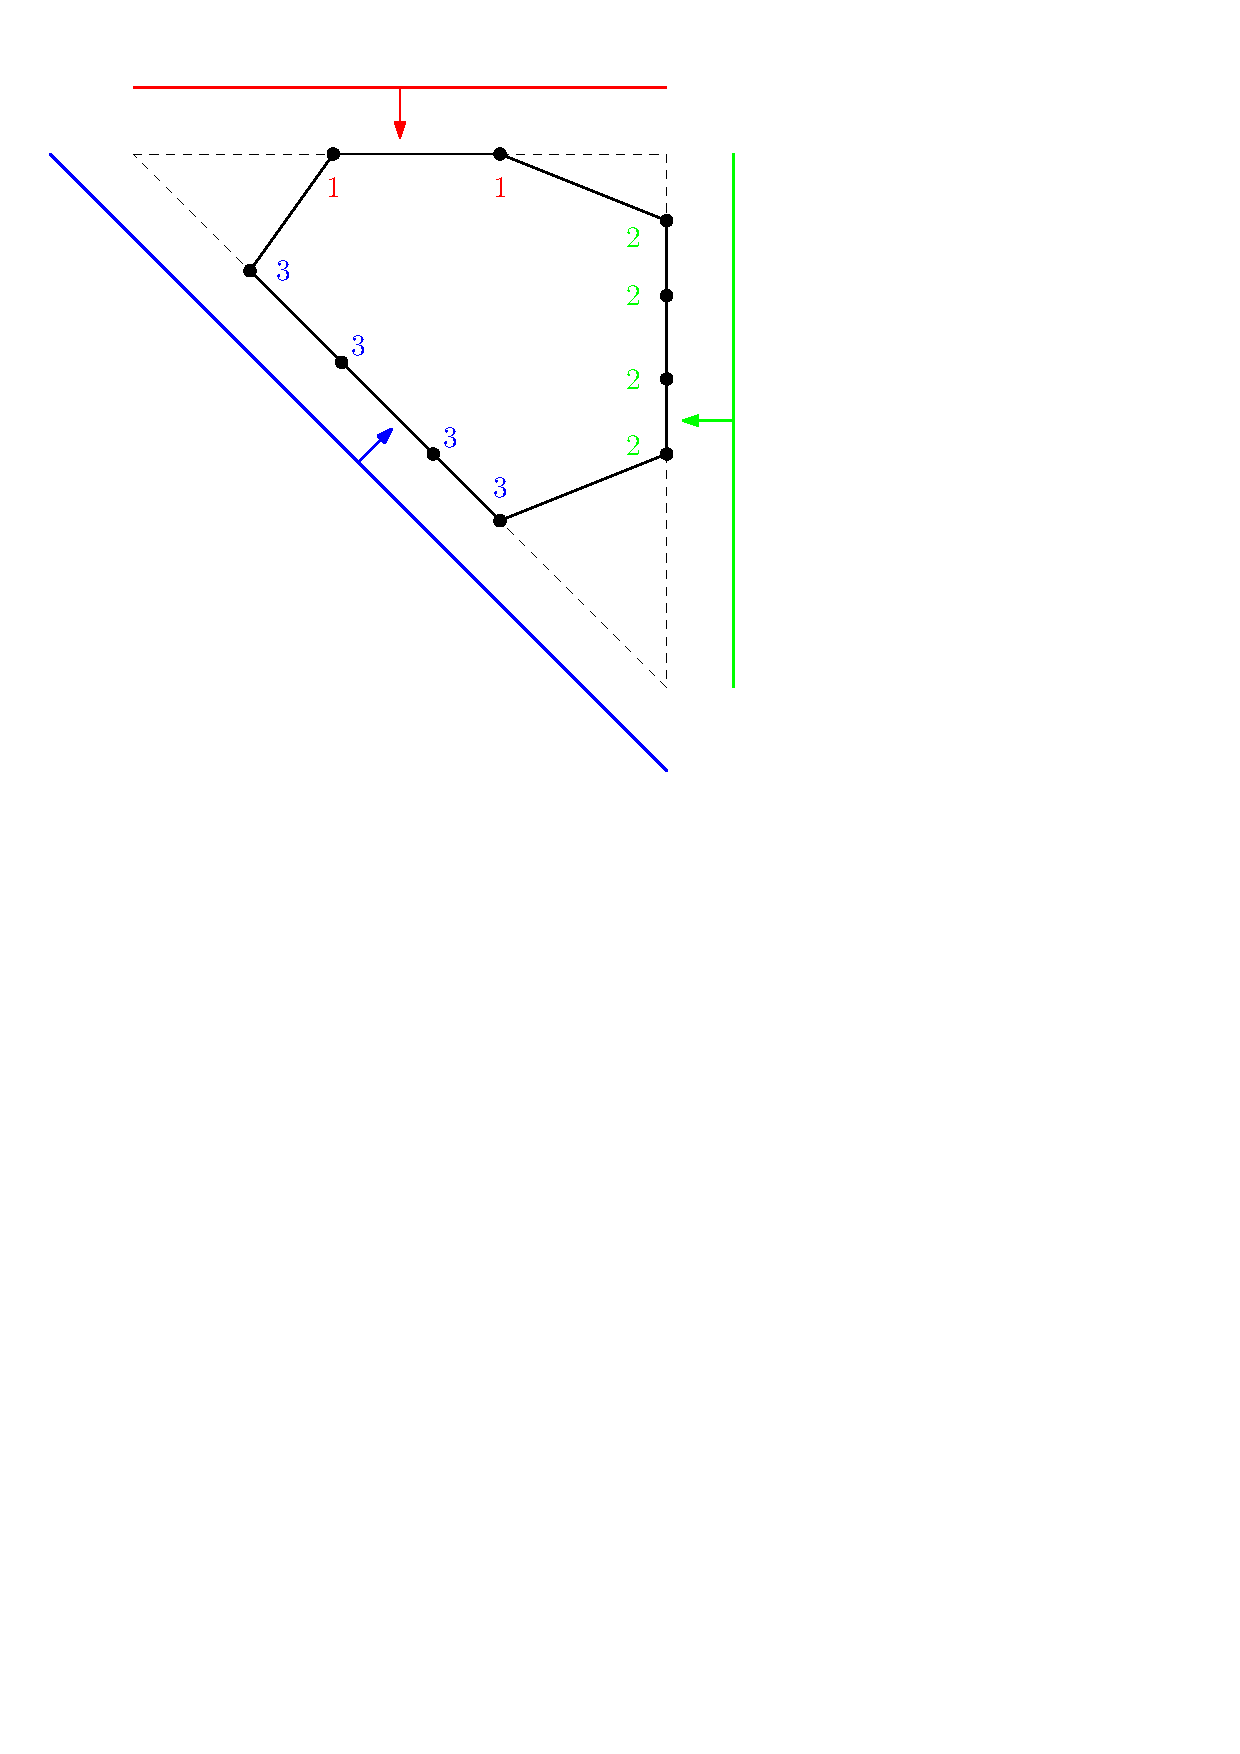
\includegraphics[width=0.8\textwidth]{sweeplines1.pdf}
    \caption{Die drei Geraden die wir von den Aufhängungen aus über den Graphen schieben.}
    \label{sweeplines1}
  \end{minipage}
  \hfill
  \begin{minipage}{0.45\textwidth}
 \centering
    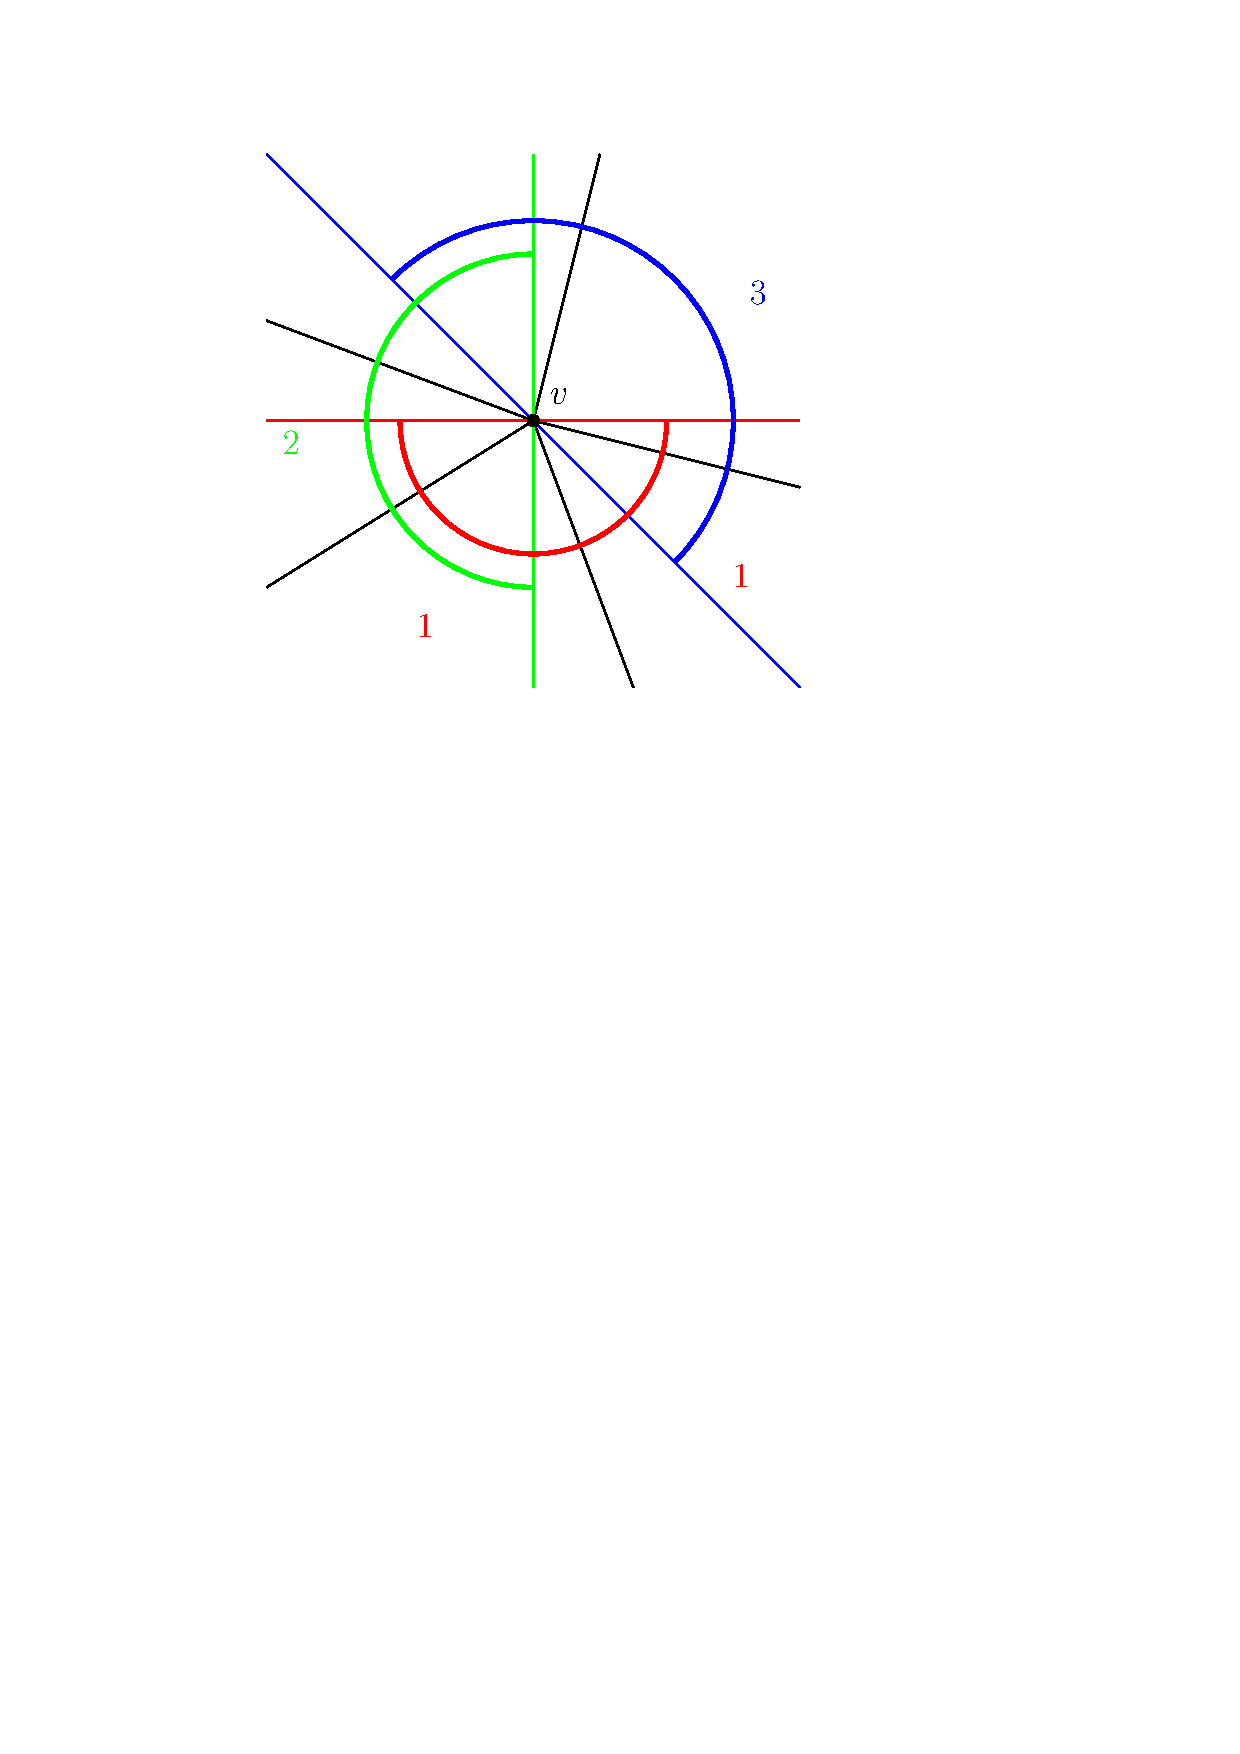
\includegraphics[width=0.8\textwidth]{sweeplines2.pdf}
    \caption{Winkel die komplett gegenüber der Geraden $i$ liegen haben Label $i$.}
    \label{sweeplines2}
  \end{minipage}
\end{figure}
\captionsetup{format=plain,labelsep=endash,justification=justified,width=1\textwidth}

Nach Beobachtung \ref{obs2} sind die Mengen $M_1,M_2$ und $M_3$ disjunkt. Wir suchen nun nach drei kombinatorisch konvexen Ecken von $\gamma$. Das FAA und das Schnyder Labeling sind Ecken kompatibel und somit hat jedes Gebiet $f \in F_{in}$ einen Winkel mit Label $i$. Also liegt in jeder Menge $M_i$ ein Knoten $v_i$, der vom FAA nicht einem Gebiet innerhalb von $\gamma$ zugewiesen wird. Nehmen wir an $a_i \notin M_i$, denn sonst hätten wir nach E1 eine Ecke gefunden. Da $D$ eine konvexe Zeichnung ist, muss $v_i$ einen Nachbarn außerhalb von $\gamma$ besitzen. Somit liegt $v_i$ auf $\gamma$, ist nicht in $\gamma$ zugewiesen und hat einen Nachbarn außerhalb von $\gamma$. Der Knoten $v_i$ erfüllt also E2. Somit hat jeder begrenzende Zykel drei kombinatorisch konvexe Ecken (jeweils eine aus jedem $M_i$).
\end{proof}

Zusammen mit Theorem \ref{com_theo} folgt, dass es sich bei dem FAA um ein Gutes-FAA handelt. Somit induziert das Ecken kompatible Paar ein SLTR von $G$.

Machen wir uns an den Beweis der Hinrichtung. Zu jedem SLTR können wir ein eindeutiges FAA erstellen, indem wir die flachen Winkel der SLTR im FAA zuweisen. Wir müssen also zeigen, dass zu jeder SLTR ein Schnyder Labeling existiert, das zusammen mit dem induzierten FAA ein Ecken kompatibles Paar bildet. Sei $G$ ein ebener, intern-3-zusammenhängender Graph mit den Aufhängungen $\{a_1,a_2,a_3\}$, der (mindestens) eine SLTR besitzt. Sei $\Delta$ eine SLTR von $G$ und sei $\phi$ das von $\Delta$ induzierte FAA.

Vor dem nächsten Lemma müssen wir zwei geometrische Objekte einführen. Beispiele finden sich in Abbildung \ref{subdividing_ex}.

\begin{definition}[Unterteilendes Dreieck]
Ein \textit{unterteilendes Dreieck} ist ein Dreieck in der Zeichnung einer SLTR von $G$, sodass gilt:
\begin{itemize}
\item Jeder Knoten auf dem Rand des Dreiecks (der keine Ecke des Dreiecks ist) ist entweder außerhalb oder innerhalb des Dreiecks zugewiesen
\item Es existiert ein Knoten (der keine Ecke ist), der keine Nachbarn außerhalb des Dreiecks hat und es existiert ein Knoten (der keine Ecke ist), der keine Nachbarn im Inneren des Dreiecks hat.
\end{itemize}
Dieses Dreieck kann Teile des Randes der Zeichnung beinhalten.
\end{definition}

\begin{definition}[teilendes Segment]
Ein \textit{teilendes Segment} eines SLTR von $G$ ist eine Menge von Kanten $\{e_1, \ldots , e_m\}$, die alle auf einer Gerade liegen, sodass gilt:
\begin{itemize}
\item Die Vereinigung der Kanten trennt die Zeichnung in zwei nichtleere Teile. 
\item Jeder innere Knoten $v$ auf dem Segment ist einem Gebiet zugeordnet, dass zwei Kanten beinhaltet die auf dem Segment liegen. Diese beiden Kanten haben $v$ als Endpunkt.
\end{itemize}
\end{definition}

\begin{figure}[h]
	\centering
	  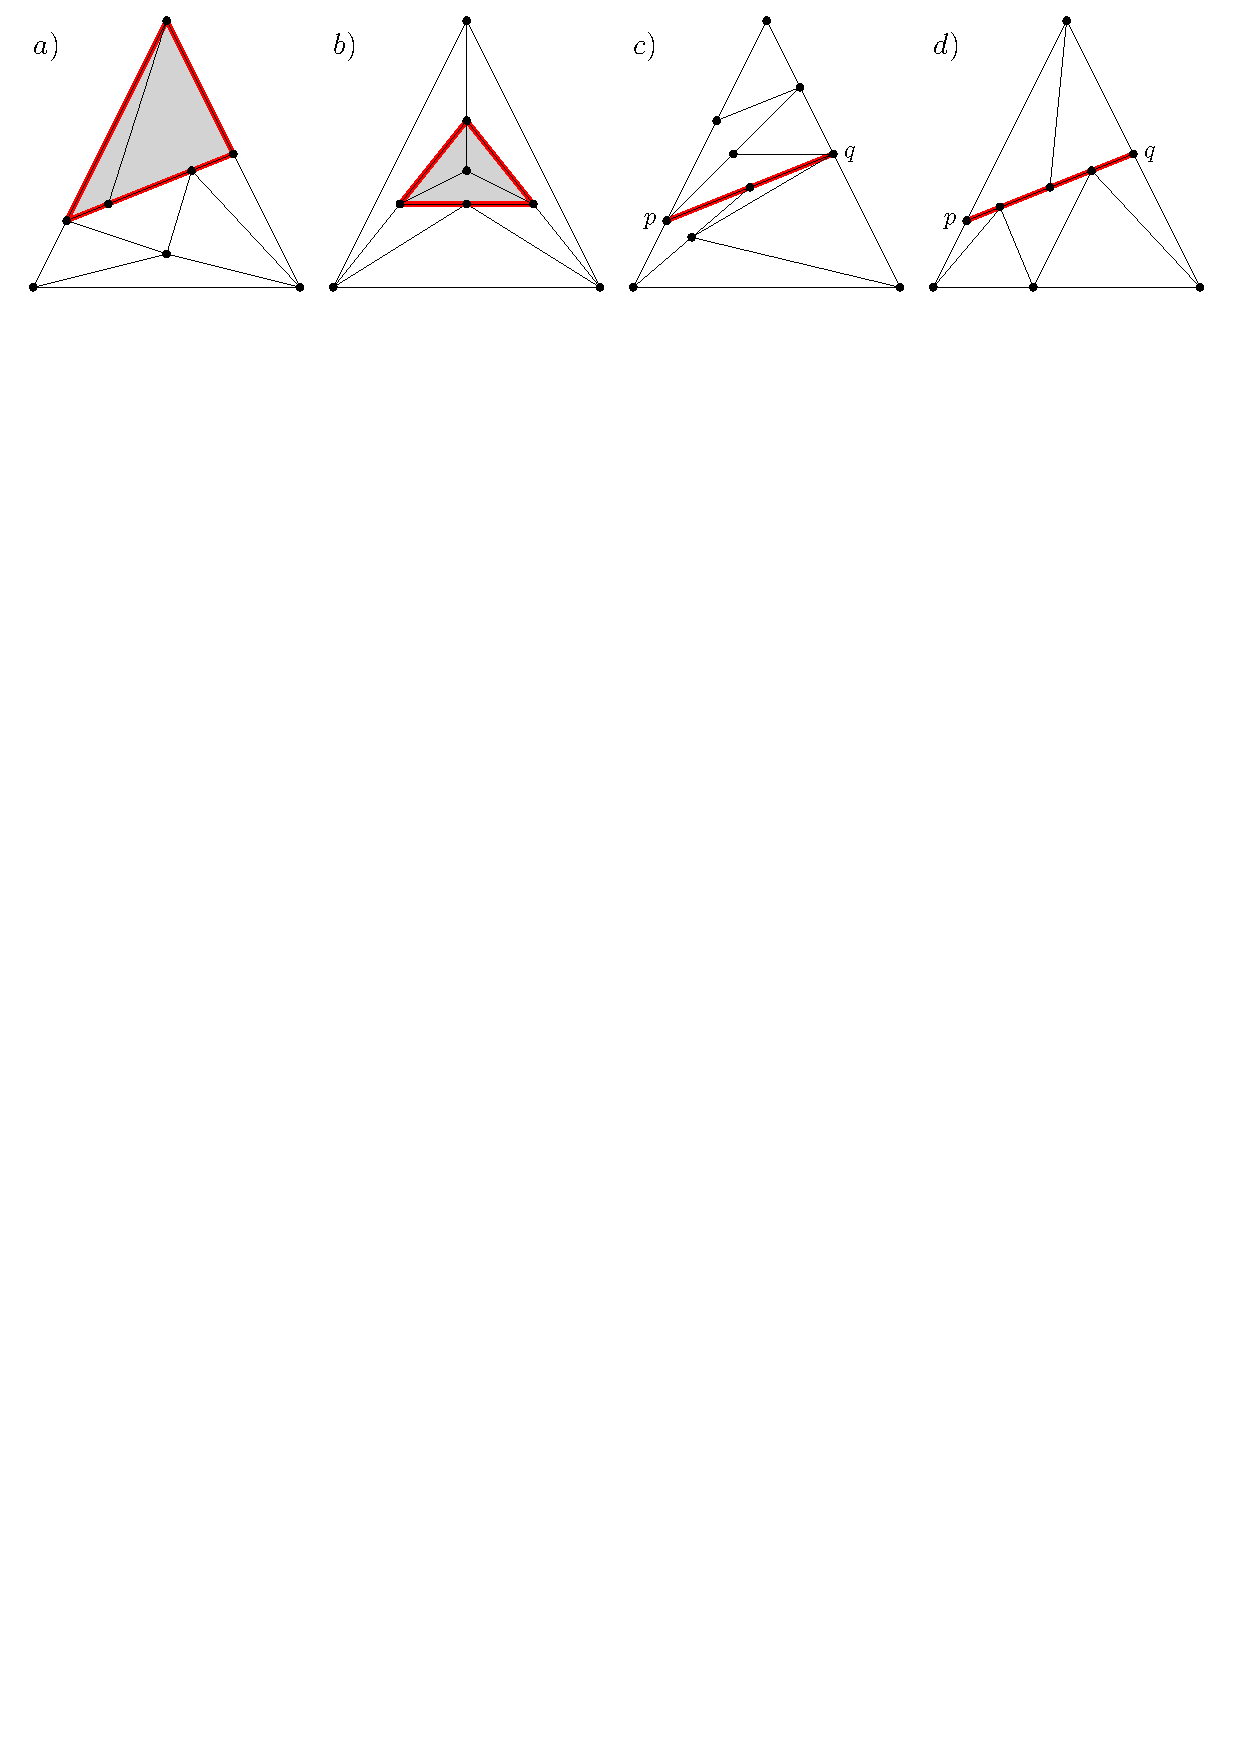
\includegraphics[width=1\textwidth]{subdividing_ex.pdf}
    	\caption{Beispiele von unterteilenden Dreiecken in a) und b) und teilenden Segmenten in c) und d) jeweils in rot.}
    	\label{subdividing_ex}
\end{figure}

Um zu zeigen, dass wir zu jeder SLTR ein passendes Ecken kompatibles Paar $(\sigma,\phi)$ finden, führen wir einen Widerspruchsbeweis durch. Sei $G$ ein kleinstmögliches Gegenbeispiel, zu dem kein Ecken kompatibles Paar existiert. Damit seien hier zuerst die minimale Anzahl an Knoten und darauf folgend die kleinste Anzahl von Kanten gemeint. Sei $\Delta$ eine SLTR von $G$, $\phi$ das induzierte FAA und $a_1,a_2$ und $a_3$ die Aufhängungen von $\Delta$.

Wir zeigen zuerst zwei Eigenschaften von $\Delta$.

\begin{lemma}\label{lem2}
Ein minimales Gegenbeispiel $\Delta$ hat kein unterteilendes Dreieck.
\end{lemma}

\begin{proof}
Nehmen wir an, dass $\Delta$ ein unterteilendes Dreieck mit den Ecken $(a,b,c)$ beinhaltet. Dies ist in Abbildung \ref{lem2} dargestellt. Seien $\Delta_1$ und $\Delta_2$ die Teile von $\Delta$, die alles außerhalb ($\Delta_1$) und innerhalb ($\Delta_2$) des Dreiecks beinhalten. Der Rand des Dreiecks $(a,b,c)$ liegt in beiden Teilen.

\begin{figure}
\centering
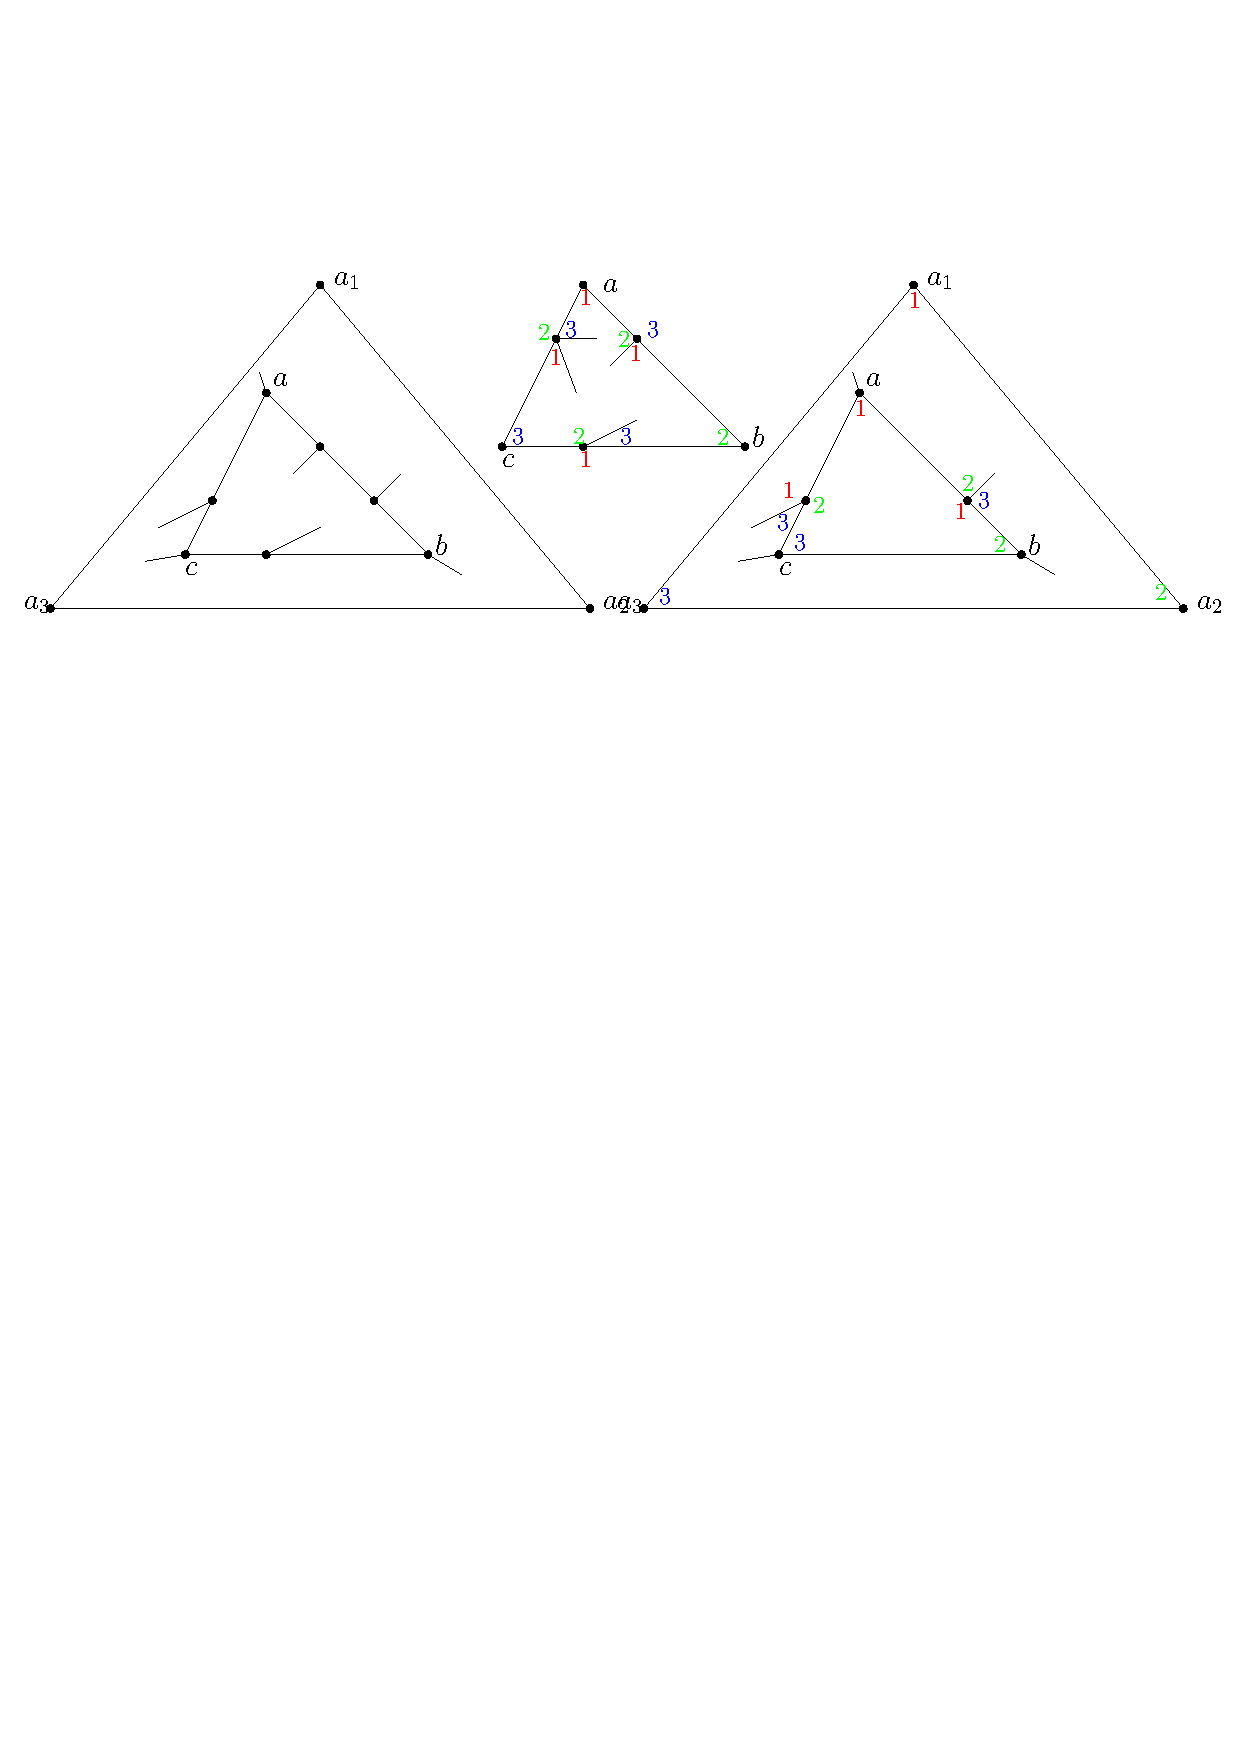
\includegraphics[width=1\textwidth]{lem2.pdf}
\caption{Wir teilen $\Delta$ in zwei Graphen und erhalten zwei Ecken kompatible Paare, die wir zusammenfügen können.}
\label{lem2}
\centering
\end{figure}

Wir ersetzen Knoten auf dem Rand des Dreiecks, die Grad 2 in $\Delta_i$ haben, mit einer Kante zwischen ihren Nachbarn. Somit sind $\Delta_1$ und $\Delta_2$ SLTRs mit weniger Knoten als $\Delta$. Da sie weniger Knoten haben als $\Delta$, können sie keine Gegenbeispiele sein und es existieren zu den SLTRs $\Delta_i$ Ecken kompatible Paare $(\sigma_i,\phi_i)$, wobei die $\phi_i$ die induzierten FAAs von $\Delta_i$ sind. Wenn wir die Paare nun zusammensetzen, dann stoßen wir auf einen Widerspruch. Die Ecken $a,b,c$ sind die Aufhängungen von $\Delta_2$. Wir wählen ihre Label so, dass sie mit den inneren Labeln des (jetzt) leeren Dreiecks in $\Delta_1$ übereinstimmen\footnote{Wir können die Label beliebig umbenennen, ohne das Schnyder Labeling zu verändern.}. Die auf diese Weise kombinierten Schnyder Labelings $\sigma_1$ und $\sigma_2$ ergeben ein Schnyder Labeling auf $G$. Die FAAs $\phi_1$ und $\phi_2$ ergeben zusammen, wenn wir die Zuweisungen an den äußeren Knoten von $\Delta_2$ und den am leeren Dreieck liegenden Knoten von $\Delta_1$ anpassen, ein FAA $\phi$ für $G$. Somit folgt die Ecken Kompatibilität aus der Tatsache, dass $(\sigma_1,\phi_1)$ und $(\sigma_2,\phi_2)$ Ecken kompatibel sind. Die SLTR $\Delta$ induziert somit ein Ecken kompatibles Paar und kann kein Gegenbeispiel sein. $\Delta$ kann kein unterteilendes Dreieck haben.
\end{proof} 

\begin{lemma}\label{lem3}
Ein minimales Gegenbeispiel $\Delta$ hat kein teilendes Segment.
\end{lemma}

\begin{remark}
Als Vorgriff auf den Beweis bedeutet dies insbesondere, dass in $\Delta$ für jede Aufhängung deg$(a_i) \geq 3$ gelten muss.
\end{remark}

\begin{proof}
Angenommen $\Delta$ hat ein teilendes Segment mit den Endpunkten $p$ und $q$. Falls auf beiden Seiten des teilenden Segmentes eine Aufhängung mit Grad größer als 2 liegt, dann wird ein unterteilendes Dreieck in $\Delta$ induziert. In diesem Fall existieren sowohl Knoten (auf dem Inneren des Segmentes), die keine Nachbarn links des teilenden Segmentes besitzten, als auch Knoten, die keine Nachbarn rechts des teilenden Segmentes besitzen. Man kann dies anhand von Abbildung \ref{subdividing_ex} d) nachvollziehen. Angenommen es handelt sich bei $p$ oder $q$ um eine Aufhängung und auf der einen Seite des Segmentes liegt nur eine Aufhängung $a_i$. Dann existiert mit $\Delta' = \Delta \backslash \{a_1\}$ ein kleineres SLTR (welches dann kein Gegenbeispiel ist) und aus diesem lässt sich ein Ecken kompatibles Paar für $\Delta$ konstruieren. Es müssen also auf beiden Seiten des Segmentes mindestens zwei Knoten liegen und somit existiert wieder ein unterteilendes Dreieck. Wir können also annehmen, dass das teilende Segment zwischen $p$ und $q$ die Aufhängung $a_1$ von Grad 2 abtrennt. $p,q$ und $a_1$ bilden somit ein Dreieck. Wir betrachten zwei Fälle. Entweder das teilende Segment besteht nur aus der Kante $(p,q)$ (Fall 1) oder es existiert mindestens ein weiterer Knoten auf dem Segment (Fall 2).

\begin{description}[leftmargin =0pt, font = \rmfamily ]
\item[Fall 1:] Das teilende Segment besteht nur aus der Kante $(p,q)$. Angenommen $q$ hat Grad 3 und $q'$ sei der dritte Nachbar von $q$. Dann existiert eine Gerade zwischen $q'$ und $p$ mit keinen Kanten in das Dreieck $p,q,q'$. Somit existiert ein unterteilendes Dreieck mit den Ecken $p,q',a_1$ (siehe Abbildung \ref{pic_lem3_1} a). Dies ist ein Widerspruch zu Lemma \ref{lem2} und es folgt $\text{deg}(p),\text{deg}(q) \geq 4$. Da $\text{deg}(a_1) = 2$ gelten muss und $G$ intern-3-zusammenhängend ist, liegt $a_1$ alleine auf der einen Seite des Segments und alle anderen Nachbarn von $p$ und $q$ auf der anderen. 
Wir behaupten, dass mindestens eine der Kanten $(a_1,p)$ und $(a_1,q)$ kontrahierbar ist, sodass der resultierende Graph eine SLTR besitzt. Die Zuweisungen des FAA bleiben, bis auf bei $p$ und $q$, gleich (siehe Abbildung \ref{pic_lem3_1} b). Dieser Schritt ist nicht trivial. Wir nutzen als Kriterium die begrenzenden Zykel aus Definition \ref{def_ccc}. Wir wollen zeigen, dass für eine der Kontraktionen wieder gilt, dass jeder begrenzende Zykel drei kombinatorisch konvexe Ecken bezüglich des FAA hat. Damit dies für keine der beiden Kontraktionen gilt, müssten zwei begrenzende Zykel $\gamma_v,\gamma_w$ mit genau drei kombinatorisch konvexen Ecken, $p,q$ und $v$ respektive $w$, existieren (siehe Abbildung \ref{pic_lem3_1} c). Nur dann induziert die Kontraktion von $(a_1,p)$ und $(a_1,q)$ jeweils einen Zykel mit nur zwei kombinatorisch konvexen Ecken. Und somit hätte der resultierende Graph keine SLTR.

Dieser Fall kann aber nicht auftreten. Seien $v,w$ die Ecken dieser Zykel. Dann existieren Pfade $P_{pw}$ und $P_{qv}$ von $p$ nach $w$ und von $q$ nach $v$. Diese Pfade sind Teil von $\gamma_v$, beziehungsweise $\gamma_w$, und enthalten somit keine kombinatorisch konvexen Ecken mit Ausnahme der Endknoten. Die Winkel an diesen Pfaden im Inneren der Zykel sind somit $\geq \pi$. Sei $z$ der Knoten an dem sich $P_{pw}$ und $P_{qv}$ kreuzen (siehe Abbildung \ref{pic_lem3_1} c). Da $z$ keine Ecke sein kann, muss $z$ auf beiden Zykeln $\gamma_v,\gamma_w$  zugewiesen sein. Somit müsste der Winkel im inneren der Zykel, der an $z$ von $P_{pw}$ und $P_{qv}$ eingeschlossen wird, mindesten $\pi$ sein. Dies ist ein Widerspruch zur Annahme das $\Delta$ eine SLTR ist (siehe Abbildung \ref{pic_lem3_1} c).

\begin{figure}
	\centering
	  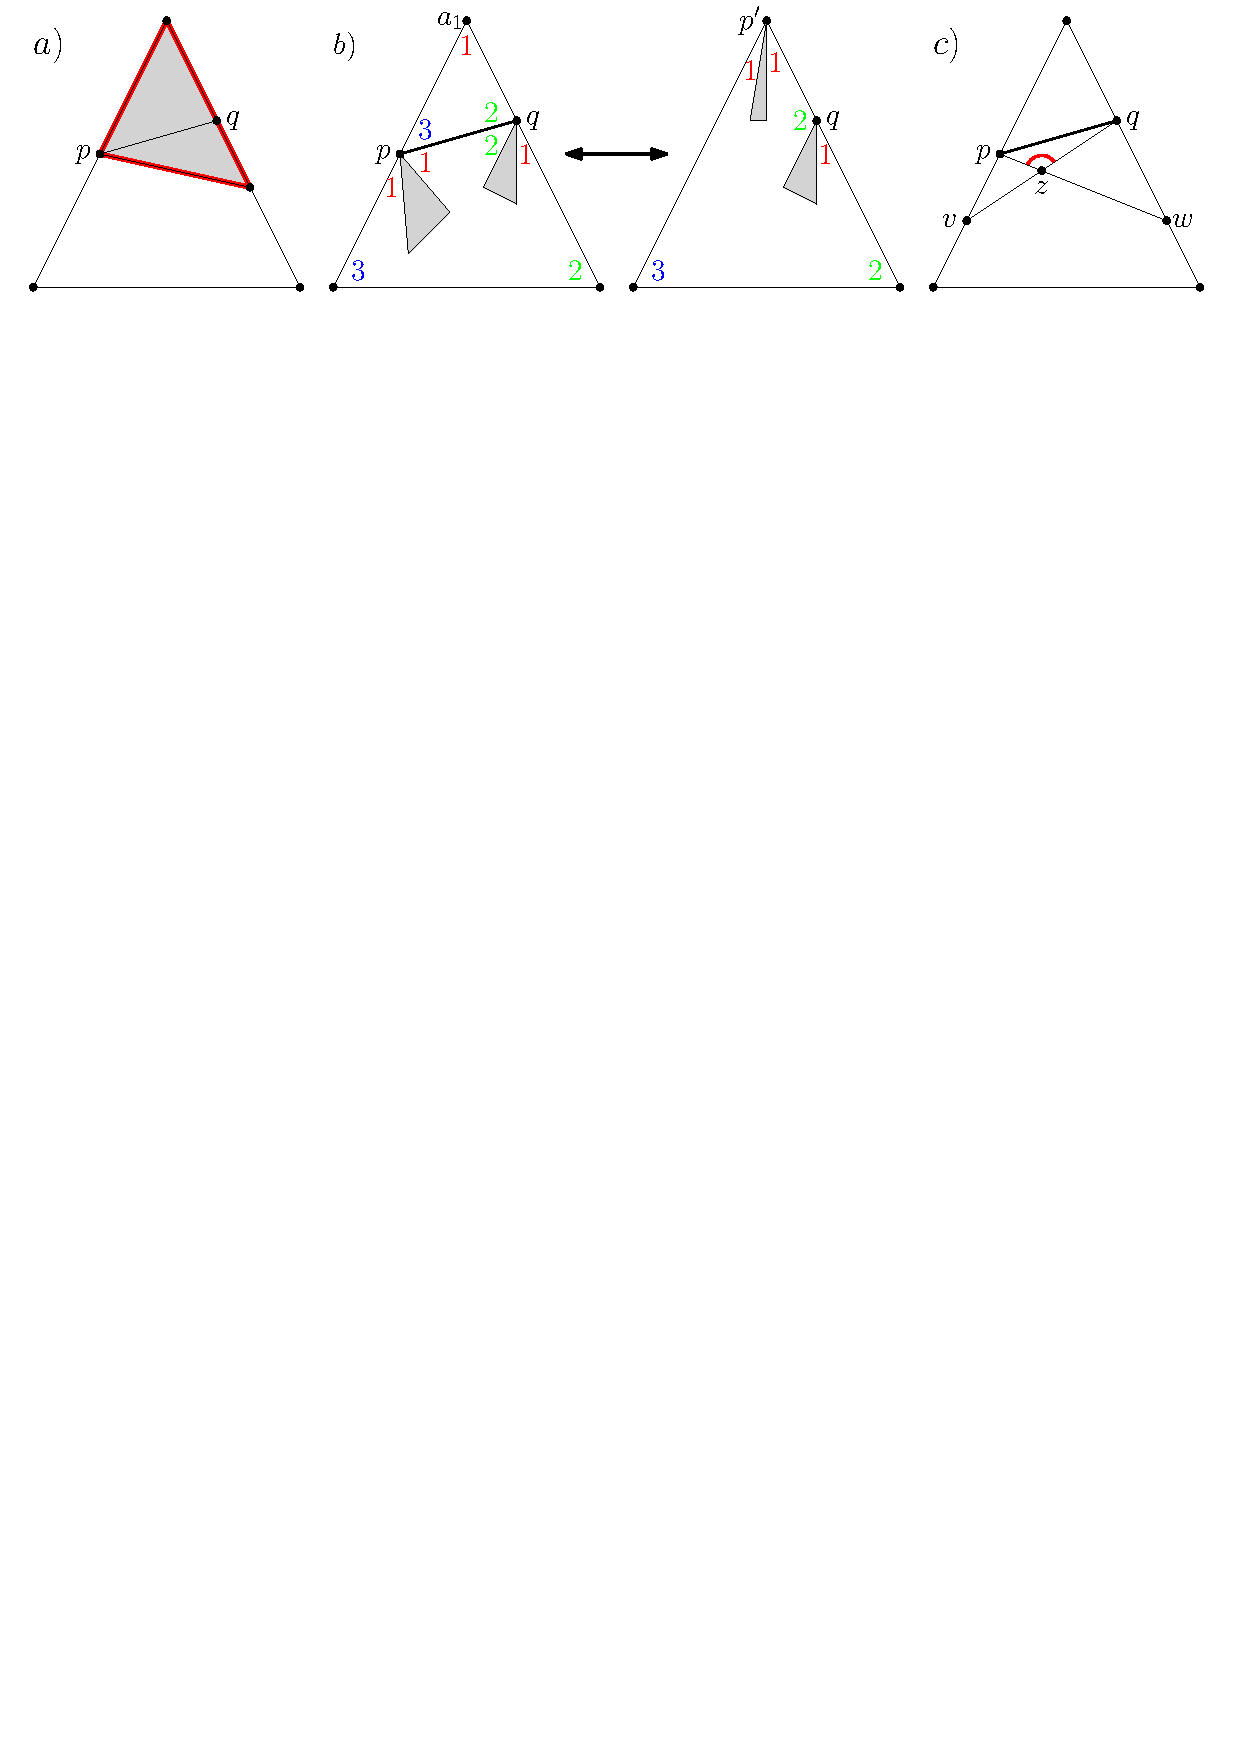
\includegraphics[width=1\textwidth]{lem3_1.pdf}
    	\caption{a) Unterteilendes Dreieck bei Grad 3. b) Kantenkontraktion der Kante $(a_1,p)$. c) Die Pfade $P_{pw}$ und $P_{qv}$, die bei der Kontraktion von $(a_1,p)$ und $(a_1,q)$ Degeneriertheit induzieren.}
    	\label{pic_lem3_1}
\end{figure}

Es kann also mindestens eine der Kanten kontrahiert werden. Sei $(a_1,p)$ diese Kante und $G'$ der Graph der durch Kontraktion von $(a_1,p)$ und das Löschen von $(p,q)$ entsteht. Wir erhalten das FAA $\phi'$ durch Löschen der Zuweisung von $p$ aus $\phi$. Der Knoten $q$ ist weiterhin dem äußeren Gebiet zugewiesen. Da $G'$ weniger Knoten als $G$ hat, ist $G'$ kein Gegenbeispiel und wir erhalten einen Schnyder Labeling $\sigma'$, das zusammen mit $\phi'$ ein Ecken kompatibles Paar bildet. Wir können $\phi'$ zu einem Labeling von $G$ erweitern, indem wir, beginnend bei $a_1$, im Uhrzeigersinn die Label $1,2$ und $3$ im Gebiet $a_1,q,p$ einfügen. Wir erhalten ein Ecken kompatibles Paar.

\item[Fall 2:] Sei $x$ der erste Nachbar von $p$ auf dem teilenden Segment. Wir kontrahieren wieder die Kante $(a_1,p)$, um $G'$ zu erhalten und zeigen, dass $G'$ eine SLTR besitzt. Bei der Kontraktion müssen keine weiteren Kanten gelöscht werden, wie in Abbildung \ref{pic_lem3_2} a) zu sehen ist. Wieder erhalten wir das FAA $\phi'$ auf $G'$, indem wir die Zuweisung von $p$ aus $\phi$ löschen. Zu jedem begrenzenden Zykel $\gamma$ in $G$ existiert ein begrenzender Zykel $\gamma'$ in $G'$. Falls $x$ eine kombinatorisch konvexe Ecke von $\gamma$ ist, dann ist $x$ dies auch für $\gamma'$, weil keine Kante an $x$ gelöscht wurde.

\begin{figure}
	\centering
	  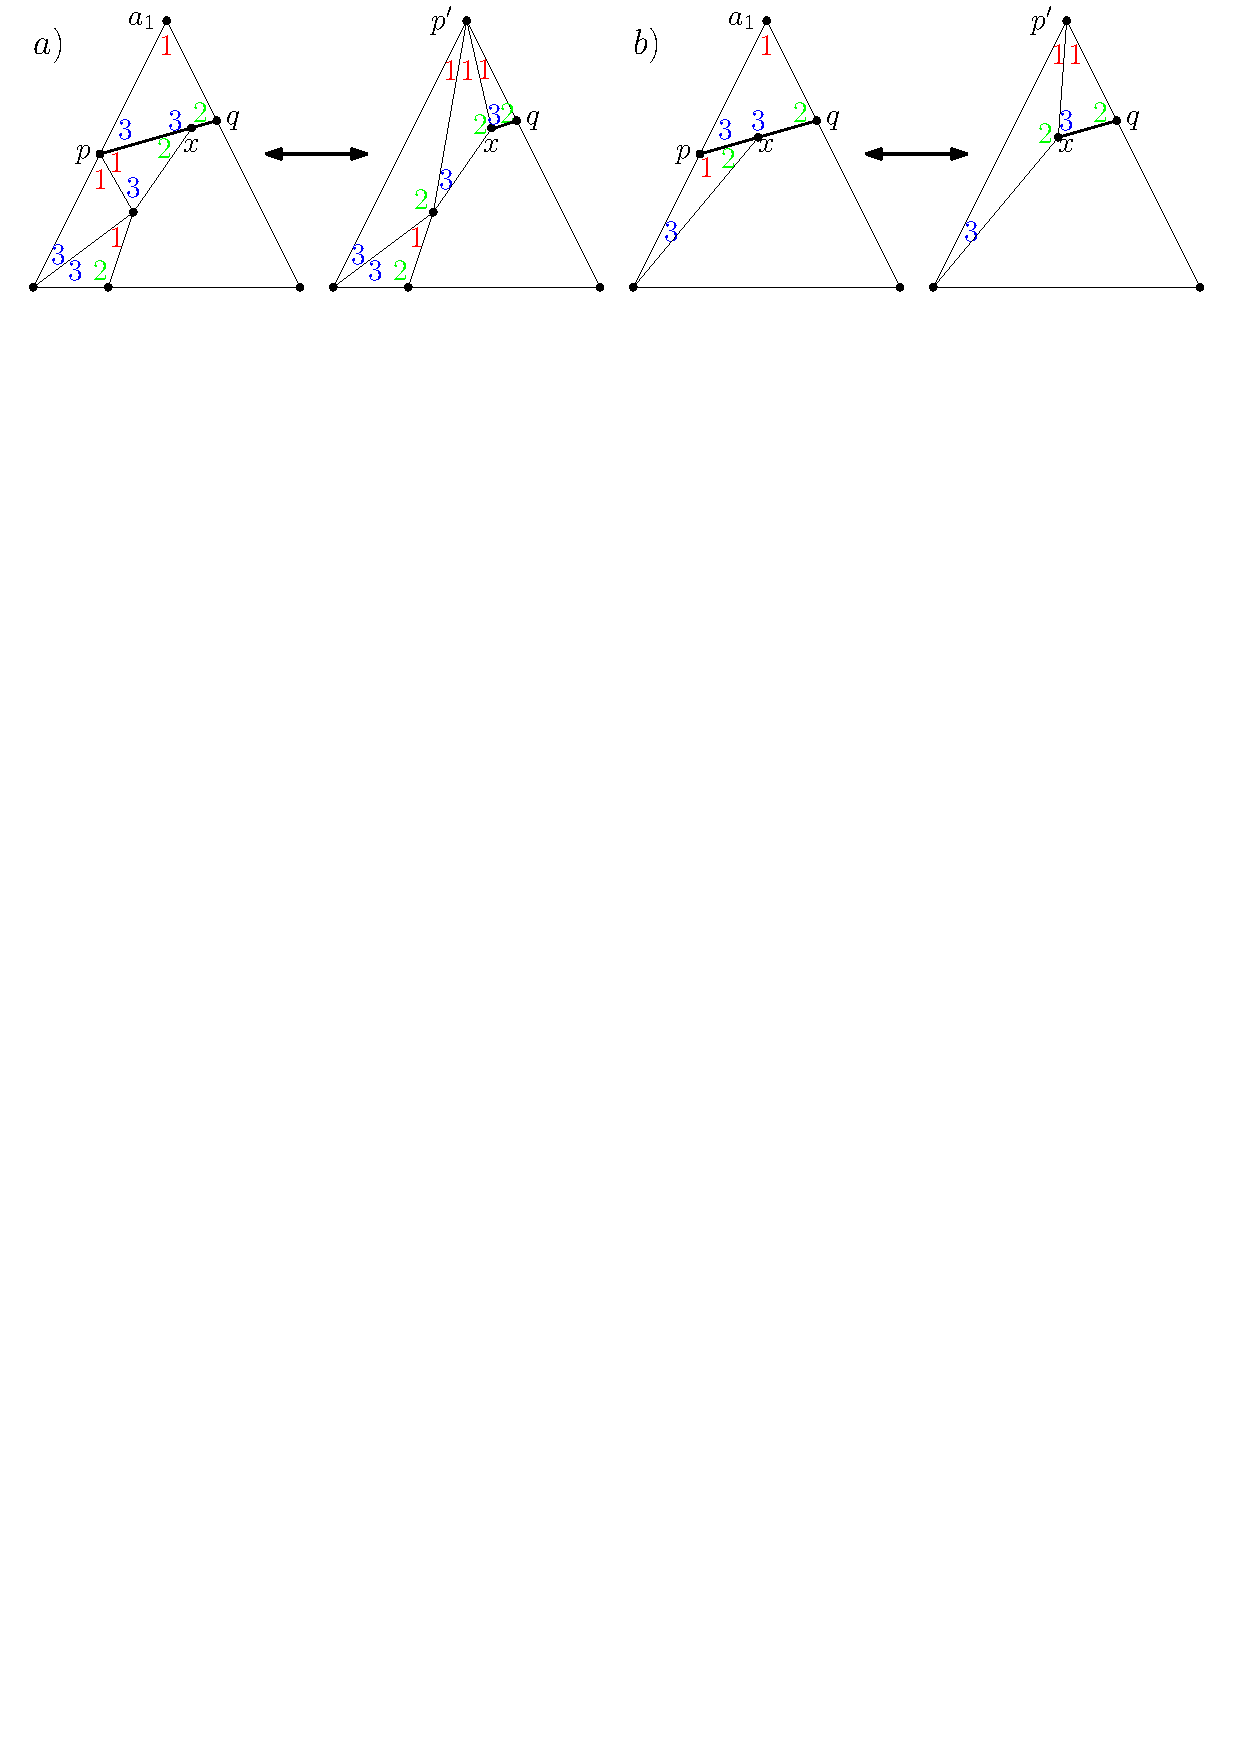
\includegraphics[width=1\textwidth]{lem3_2.pdf}
    	\caption{Zwei Beispiele zur Kontraktion von $(a_1,p)$ mit passendem Schnyder Labeling im zweiten Fall.}
    	\label{pic_lem3_2}
\end{figure}

Nun ist $G'$ kein Gegenbeispiel und es existiert ein zu $\phi'$ kompatibles Schnyder Labeling $\sigma'$. $\sigma'$ ist erweiterbar zu einem Labeling $\sigma$ für $G$. Füge Label 1 bei $a_1$ und 3 bei $p$ ein. $\Delta$ kann also kein teilendes Segment haben.
\end{description}
\end{proof}

Im nächsten Lemma wird eine Eigenschaft von Ecken kompatiblen Paaren festgehalten, die für den Beweis von Theorem \ref{theo_ccc} nützlich sein wird.

\begin{lemma}\label{lem4}
Sei G ein ebener, intern-3-zusammenhängender Graph mit den Aufhängungen $\{a_1,a_2,a_3\}$ und einem Ecken kompatiblen Paar $(\sigma,\phi)$ aus einem Schnyder Labeling und einem FAA. Sei $v$ ein Nachbar einer Aufhängung $a_i$. Falls $v$ von $\phi$ einem Gebiet $f$ zugewiesen ist, das $a_i$ beinhaltet, folgt, dass das Label von $v$ in $f$ nur einmal an $v$ vorkommt. Alle anderen Winkel an $v$ haben ein anderes Label.
\end{lemma}

\begin{figure}[h]
\centering
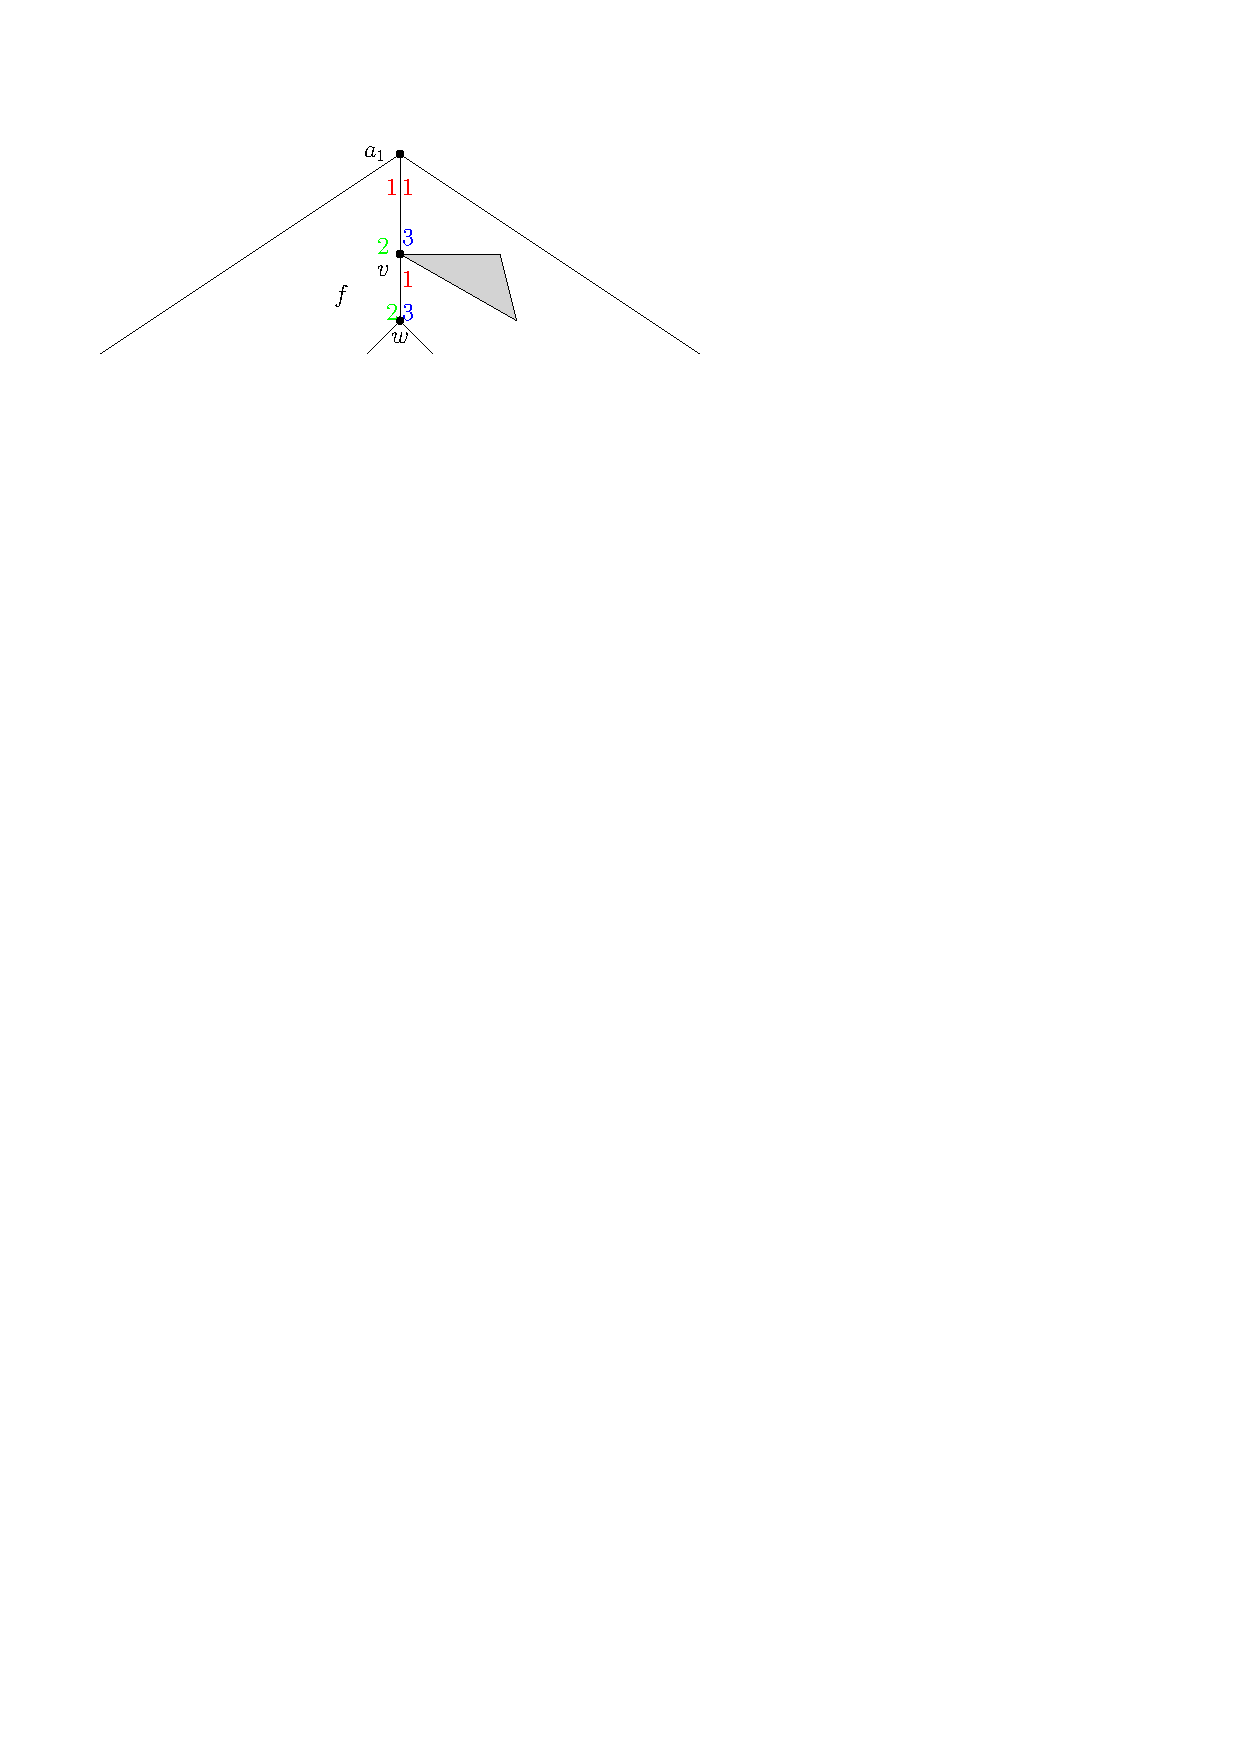
\includegraphics[width=0.65\textwidth]{lem4.pdf}
\caption{Das Label 2 kann an $v$ nur einmal vorkommen.}
\label{lem4}
\centering
\end{figure}

\begin{proof}
Nehme ohne Beschränkung der Allgemeinheit an, dass $v$ ein Nachbar von $a_1$ ist und $v$ dem Gebiet $f$ auf der linken Seite der Kante $(a_1,v)$ zugeordnet ist (siehe Abbildung \ref{lem4}). Sei $w$ der andere Nachbar von $v$ in $f$. Die Kante $(a_1,v)$ hat zweimal Label 1, jeweils links und rechts von $a_1$, und Label 2 am zugewiesenen Winkel von $v$. Nach Definition \ref{def_sl} muss an jeder Kante jedes Label einmal vorkommen. Somit ist das letzte Label an $(a_1,v)$ von Typ 3. Da $(\sigma,\phi)$ ein kompatibles Paar ist, muss der Winkel von $w$ in $f$ ebenfalls Label 2 haben, da sonst keine Ecke mit Label 2 existiert (vergleiche Definition \ref{def_sw}). Um die Kante $(v,w)$ müssen ebenfalls alle Label vorkommen und somit müssen wir 1 und 3 (wie in der Abbildung \ref{lem4}) einfügen. Um $v$ existieren nach L2 im Uhrzeigersinn drei nichtleere Intervalle mit Label 1, 2 und 3. Folglich können die verbliebenen unbekannten Label an $v$ nur von Typ 1 oder 3 sein.
\end{proof}

\begin{lemma}\label{lem5}
In einem minimalen Gegenbeispiel $\Delta$ kann kein Nachbar $x_i$ einer der Aufhängungen $a_i$ einem Gebiet zugeordnet sein, zu dessen Rand die Kante $(a_i,x_i)$ gehört.
\end{lemma}

\begin{remark}
Lemma \ref{lem5} impliziert insbesondere, dass die drei Aufhängungen $a_1,a_2$ und $a_3$ von $\Delta$ ein Dreieck bilden. Es liegen also keine weiteren Knoten auf dem äußeren Rand von $\Delta$.
\end{remark}

\begin{proof}
Angenommen es existiert ein Nachbar $x$ von $a_1$, der dem Gebiet $f$ zugewiesen ist und $a_1$ liegt auf dem Rand von $f$. Somit tut dies auch die Kante $(a_1,x)$. Wir werden wieder einen kleineren Graphen $G'$ erstellen und zeigen, dass $G'$ eine SLTR zulässt. Das zu diesem SLTR korrespondierende Schnyder Labeling $\phi'$ werden wir zu einem Schnyder Labeling von $G$ erweitern. Im besten Fall kontrahieren wir die Kante $(a_1,x)$, um $G'$ zu erhalten, doch dies ist nicht immer möglich. Ein Beispiel ist in Abbildung \ref{pic_lem5_1} a) zu sehen. Wenn $z$ nur Grad 3 hat, dann wäre $G'$ nach der Kontraktion nicht mehr intern-3-zusammenhängend.

Sei $z$ die dritte Ecke des Gebietes $f$ mit den Ecken $a_1$ und $x$ in der Zeichnung $\Delta$. Es kann nur ein solches $z$ geben, da sonst (wie in Abbildung \ref{pic_lem5_1} a) ein unterteilendes Dreieck in $\Delta$ existieren müsste. Wir haben aber in Lemma \ref{lem2} gezeigt, dass dies nicht der Fall sein kann.

Wir können annehmen, dass $z$ und $a_1$ benachbart sind. Falls nicht, muss ein Knoten $x'$ zwischen $z$ und $a_1$ liegen. Sei $z'$ die dritte Ecke im Gebiet mit Ecken $a_1,x',z'$. Der Knoten $x'$ muss in diesem Gebiet eine Ecke sein, da er im zuvor betrachteten Gebiet zugewiesen ist (siehe Abbildung \ref{pic_lem5_1} b). Nun ist entweder $z'$ ein Nachbar von $a_1$, oder wir führen diesen Schritt noch einmal durch und finden $x''$. Da $a_1$ endlich viele Nachbarn hat, können wir den Schritt nur endlich oft durchführen. Es existiert also ein Gebiet mit $a_1, x$ und $z$ als Ecken und $x$ und $z$ sind Nachbarn von $a_1$. Es sei angemerkt, dass $x$ am äusseren Gebiet von $G$ liegen kann.

\begin{figure}[h]
	\centering
	  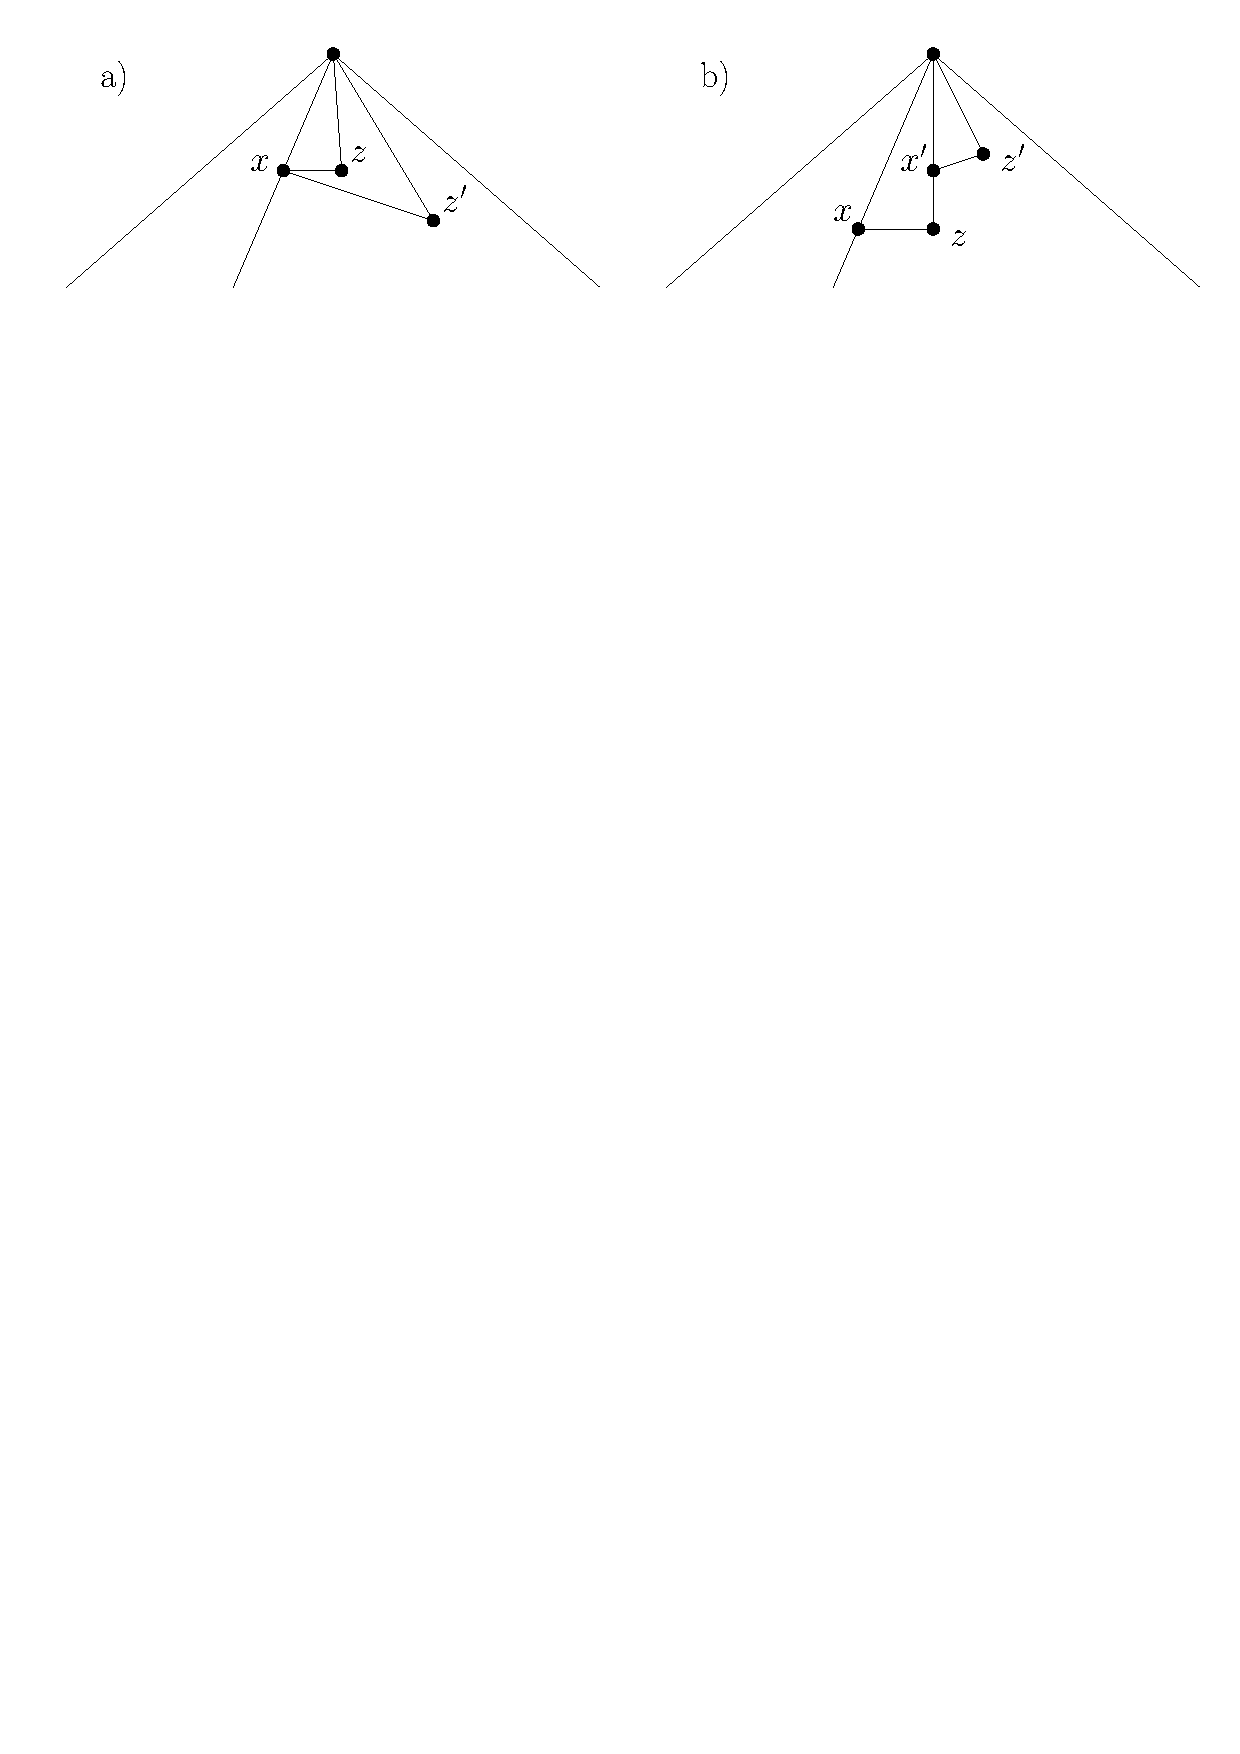
\includegraphics[width=0.8\textwidth]{lem5_1.pdf}
    	\caption{a) Es können keine zwei Knoten mit geradlinigen Pfaden zu $x$ und $a_1$ existieren. b) Falls $a_1$ kein Nachbar von $z$ ist, dann müssen die Knoten $x'$ und $z'$ existieren.}
    	\label{pic_lem5_1}
\end{figure}

Wir werden je nach Fall unterschiedliche Ansätze wählen, um $G'$ zu erzeugen. Es folgt eine Übersicht der Fälle, die in Abbildung \ref{pic_lem5_2} skizziert sind.

\begin{itemize}
\item [1.] Wenn $x$ und $z$ Nachbarn sind:
	\begin{itemize}
	\item [a)] Und $z$ dem Gebiet auf der anderen Seite von $(x,z)$ zugewiesen ist, dann kontrahieren wir $(x,z)$.
	\item [b)] Falls sonst $\text{deg}(z)$=3 gilt, löschen wir $z$ und fügen eine passende Kante ein.
	\item [c)] Falls sonst $(a_1,x)$ kontrahierbar ist, wird sie kontrahiert.
	\item [d)] Sonst wird die Kante $(a_1,z)$ gelöscht.
	\end{itemize}
\item [2.] Wenn $x$ und $z$ keine Nachbarn sind, dann kontrahieren wir die Kante $(a_1,x)$.
\end{itemize} 

\begin{figure}
	\centering
	  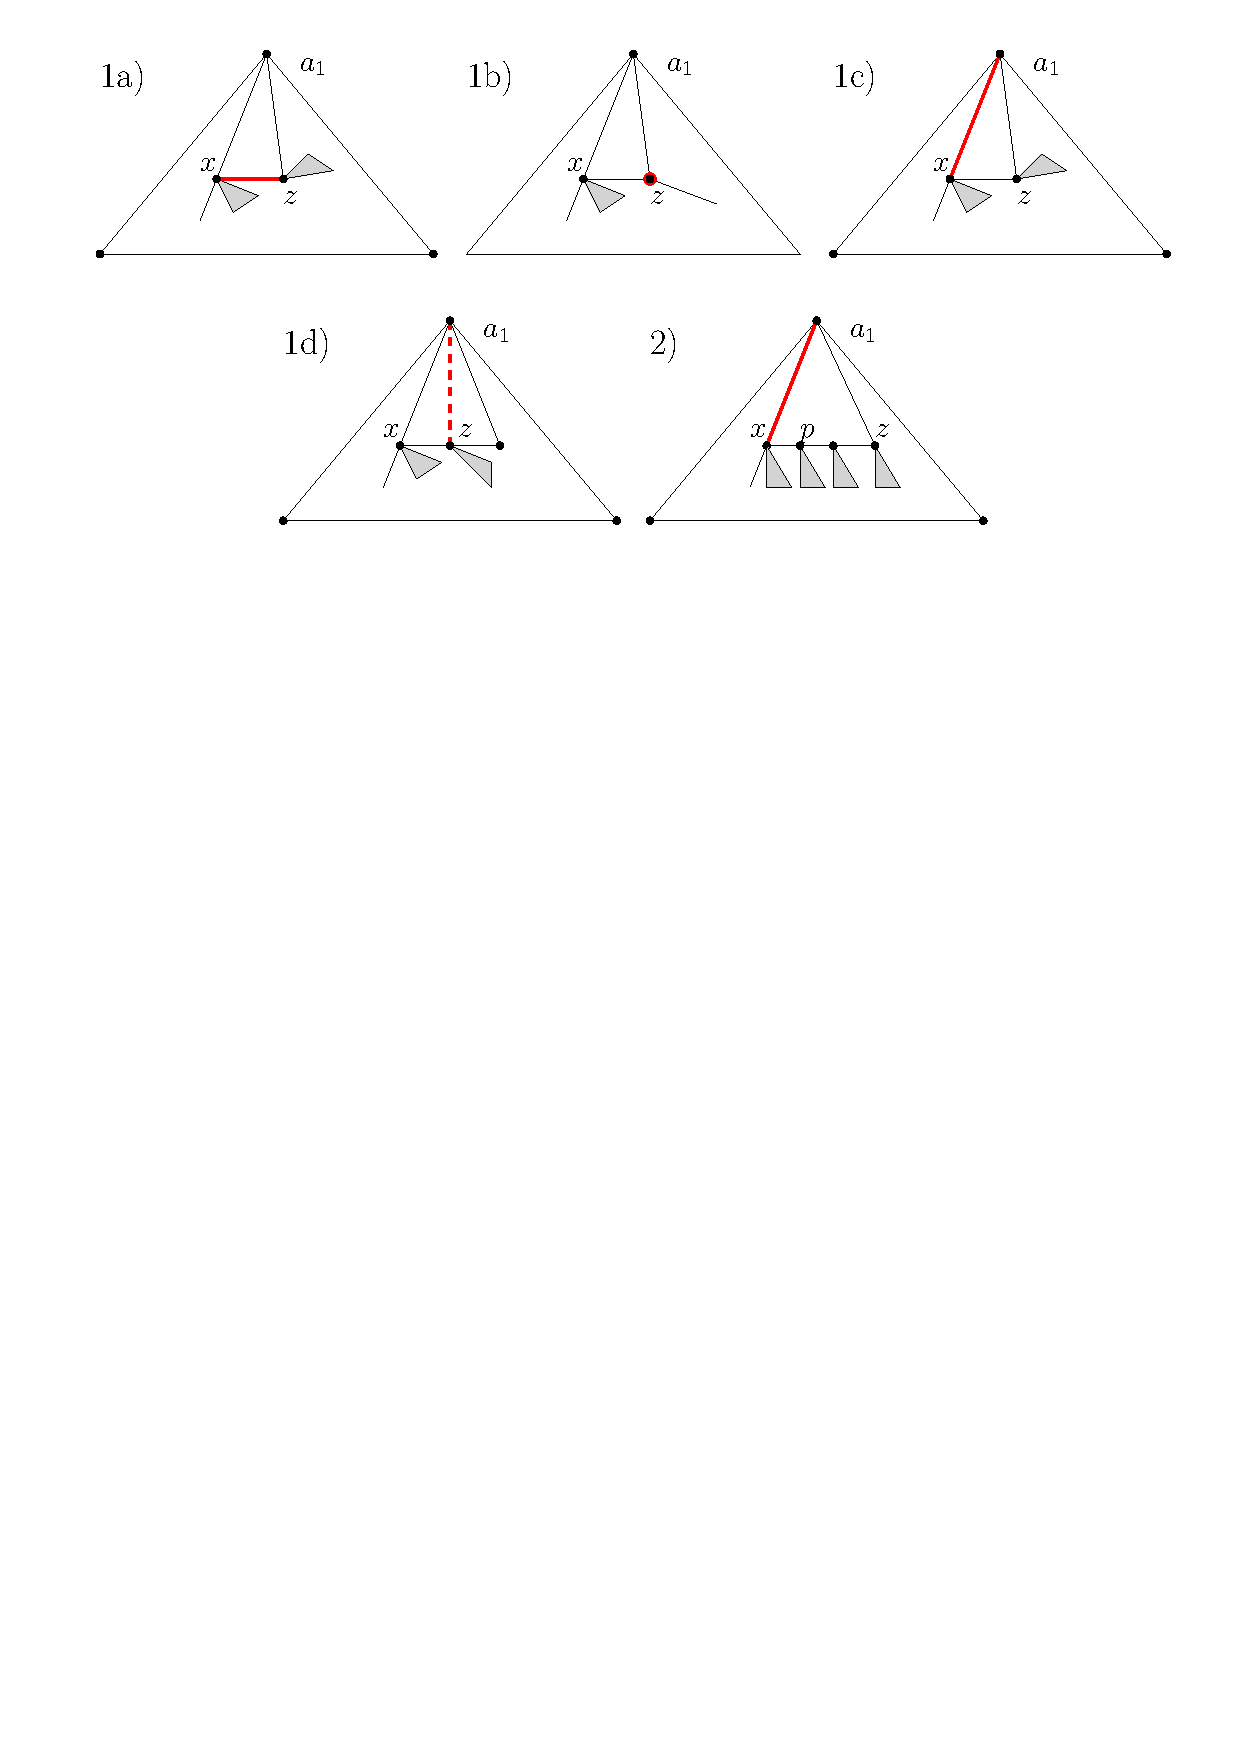
\includegraphics[width=0.8\textwidth]{lem5_2.pdf}
    	\caption{Die möglichen Fälle bei der Erzeugung von $G'$. Die durchgezogenen roten Kanten werden kontrahiert. Der rote Knoten und die gestrichelte rote Kante werden gelöscht.}
    	\label{pic_lem5_2}
\end{figure}

Für jeden dieser Fälle entsteht ein Graph $G'$, der kleiner ist als $G$. Wir werden zeigen, dass er eine SLTR hat, und da er kein Gegenbeispiel sein kann, besitzt er ein Ecken kompatibles Paar. Wir werden das Schnyder Labeling von $G'$ zu einem von $G$ erweitern und zeigen, dass dieses Ecken kompatibel mit dem von $\Delta$ induzierten FAA ist. Wir wenden uns nun den einzelnen Fällen im Genauen zu. 

Im Folgenden seien $x$ und $z$ benachbart. Das Dreieck $f_{a_1zx}$ in $\Delta$ hat somit keine weiteren Knoten auf den Rändern.
\begin{description}[leftmargin =0pt, font = \rmfamily ]
\item[Fall 1a:] Wir erzeugen $G'$, indem wir die Kante $(a_1,z)$ löschen und $(x,z)$ kontrahieren. Wir bezeichnen den neuen Knoten mit $x'$ (siehe Abbildung \ref{pic_lem5_3} 1b). Wir erhalten das FAA $\phi'$ von $G'$, indem wir die Zuweisung von $x$ aus $\phi$ löschen. Sei $\gamma'$ ein begrenzender Zykel in $G'$. Betrachte den induzierten Zykel $\gamma$ in $G$. Dieser hat mindestens drei kombinatorisch konvexe Ecken. Diejenigen Ecken, die nicht $x$ und $z$ sind, müssen auch Ecken von $\gamma'$ sein. Falls entweder $x$ oder $z$ eine kombinatorisch konvexe Ecke von $\gamma$ ist, dann ist $x'$ eine kombinatorisch konvexe Ecke von $\gamma'$. Angenommen $x$ und $z$ sind beide kombinatorisch konvexe Ecken von $\gamma$. Merke, dass es sich bei $\gamma$ nicht nur um das Dreieck $f_{a_1zx}$ handeln kann, da $\gamma'$ nicht von einem Pfad induziert wird. Somit muss entweder an $x$ oder $z$ mindestens ein weiterer Winkel im Inneren von $\gamma$ liegen. Angenommen ein Winkel an $z$, aber nicht der im Dreieck $f_{a_1zx}$, liegt im Inneren von $\gamma$. Dann zeigt dieser Winkel nicht in Richtung von $x$. Somit muss der zugewiesene Winkel an $z$ im Inneren von $\gamma$ liegen (wie in Abbildung \ref{pic_lem5_3} a). Es folgt, dass $\gamma$ mindestens vier kombinatorisch konvexe Ecken in $G$ hat. Falls $\gamma$ einen weiteren Winkel an $x$ in seinem Inneren hat, dann kann man analog zeigen, dass $\gamma$ wieder mindestens vier kombinatorisch konvexe Ecken in $G$ hat. Somit hat $G'$ eine SLTR.

\begin{figure}
\centering
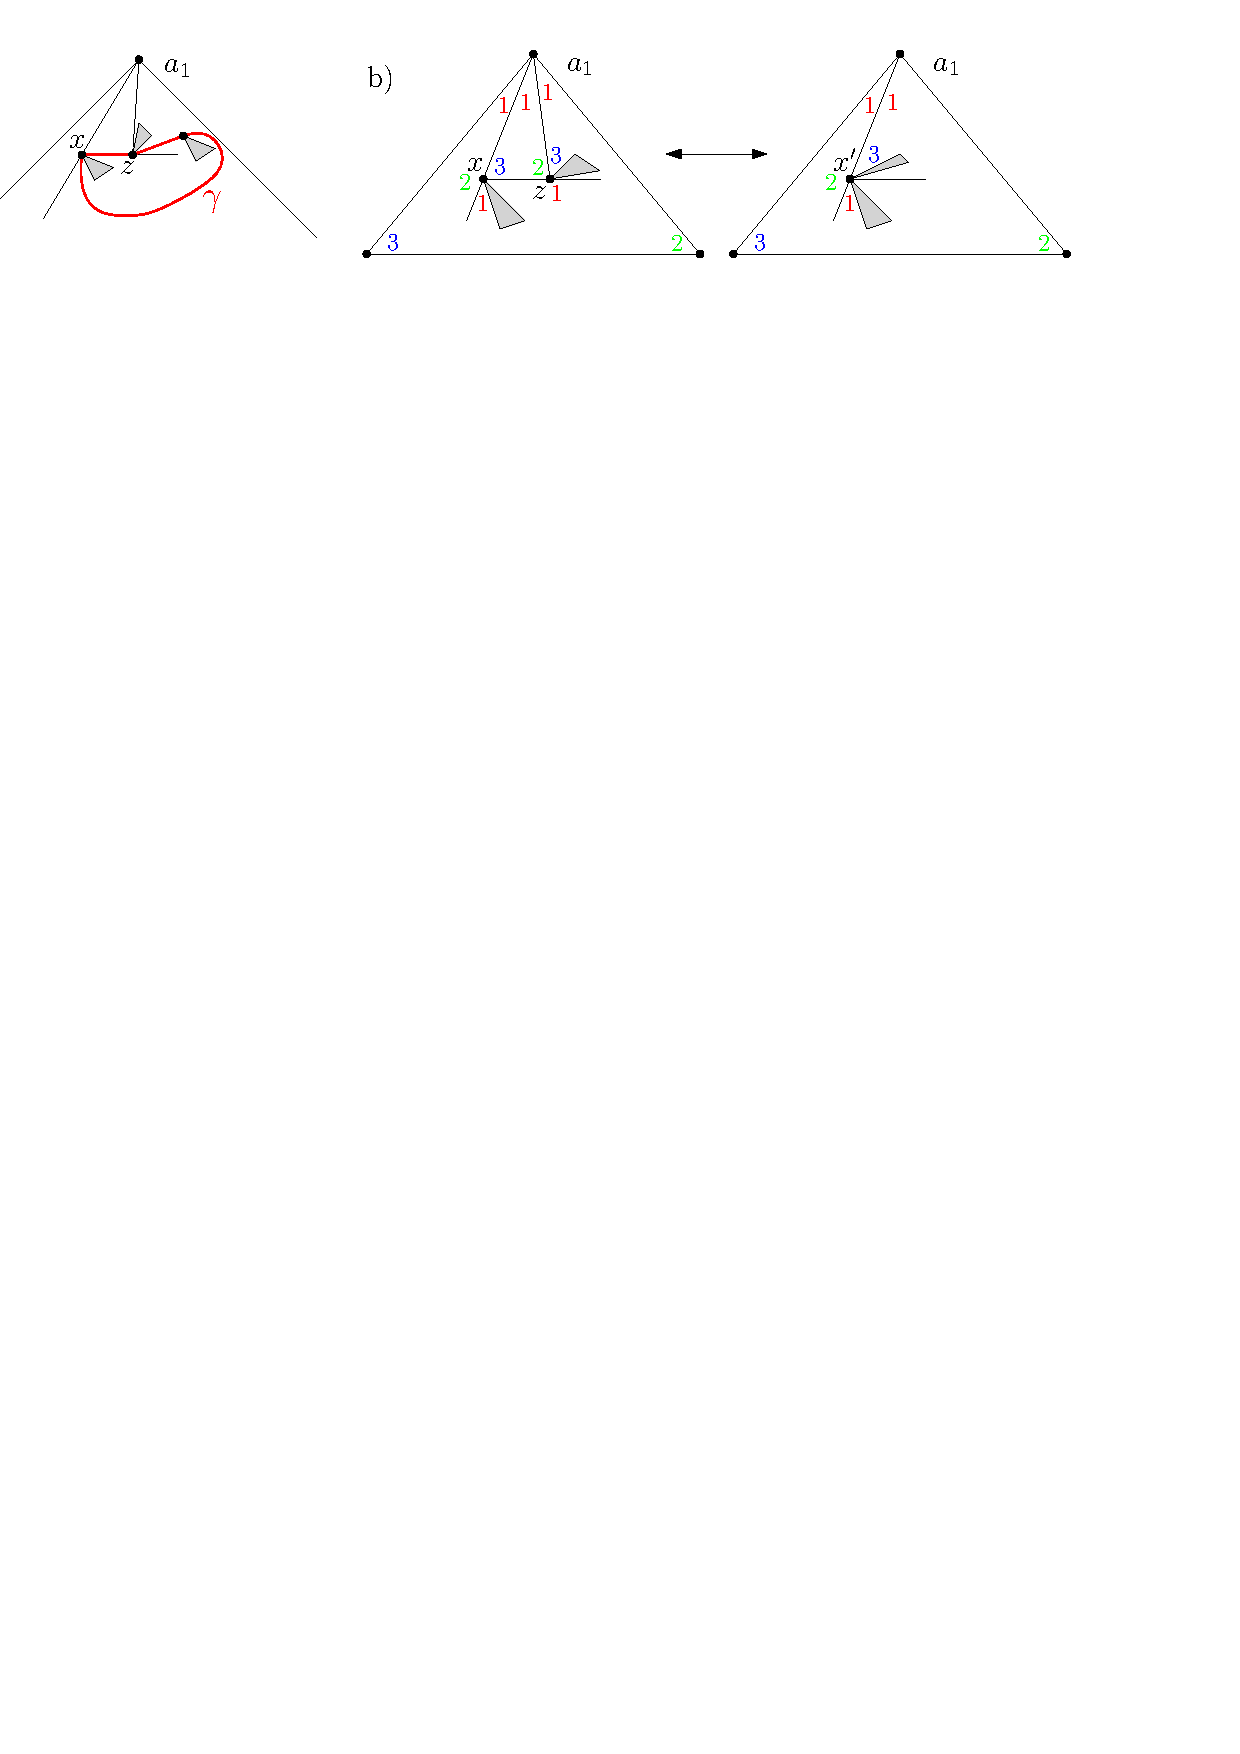
\includegraphics[width=1\textwidth]{lem5_3.pdf}
\caption{a) Es existiert ein weiterer Winkel im Inneren von $\gamma$. b) Wir erhalten $G'$ durch Kontraktion der Kante $(x,z)$.}
\label{pic_lem5_3}
\end{figure}

Da $G'$ weniger Knoten als $G$ hat, kann es kein Gegenbeispiel sein. Sei $\sigma'$ ein zu $\phi'$ Ecken kompatibles Schnyder Labeling. Nach Lemma \ref{lem4} kommt das Label des zugewiesenen Winkels an $x'$ nur einmal vor. Wir kehren nun die Kontraktion von $(x,z)$ um (vergleiche Abbildung \ref{pic_lem5_3} b). Die Winkel von $a_1,x$ und $z$ im Dreieck $f_{a_1zx}$ haben Label 1, 2 und 3 im Uhrzeigersinn bei $a_1$ beginnend. Wir geben dem zugewiesenen Winkel an $z$ Label 1. Der Winkel an $z$, dem wir ein neues Label gegeben haben, ist keine Ecke und sonst hat sich im Bezug auf $\phi'$ nichts verändert. Somit ist das konstruierte Schnyder Labeling $\sigma$ Ecken kompatibel zu $\phi$. $G$ kann also kein Gegenbeispiel sein.

\item[Fall 1b:] Der Knoten $z$ habe Grad 3. Falls der Knoten $z$ von $\phi$ zugeordnet ist, dann kann er keinem zu $(x,z)$ adjazenten Gebiet zugeordnet sein (wegen Fall 1a). Angenommen $z$ ist einem Gebiet zugeordnet, zu dem, wie in Abbildung \ref{pic_lem5_4}, $a_1$ gehört. Dann existiert ein unterteilendes Dreieck. Die gestrichelte Gerade muss in $\Delta$ existieren, weil $z$ Grad 3 hat. Somit ist $G$ kein Gegenbeispiel . Der Knoten $z$ kann also nicht zugewiesen sein.

\begin{figure}[h]
	\centering
	  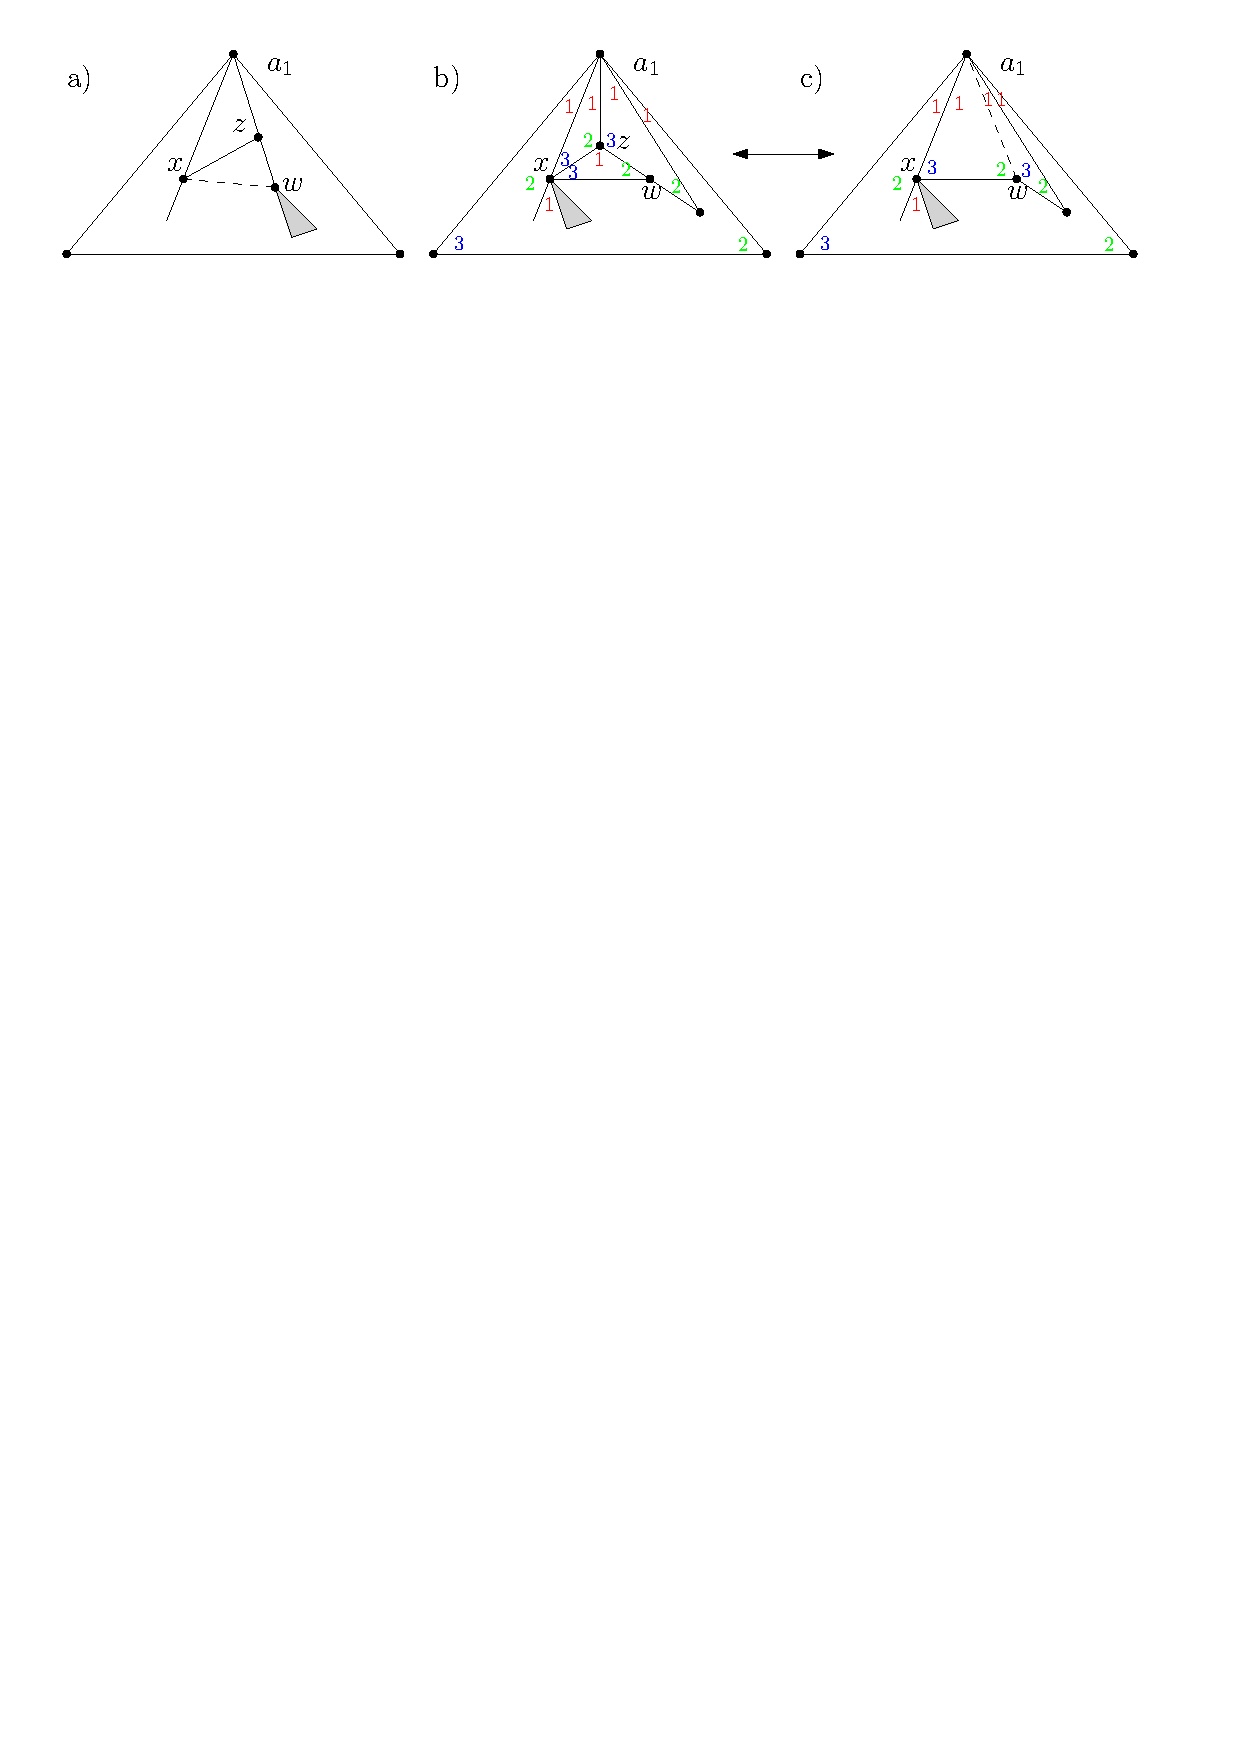
\includegraphics[width=1\textwidth]{lem5_4.pdf}
\caption{a) Falls $w$ dem Gebiet mit $a_1$ zugewiesen ist, existiert ein unterteilendes Dreieck. b),c) Das Löschen von $z$, falls $w$ dem Gebiet mit $a_1$ zugewiesen ist oder wenn $w$ Grad 3 hat. }
    	\label{pic_lem5_4}
\end{figure}

Sei $w$ der dritte Nachbar von $z$. Dieser muss zugewiesen sein, da sonst wieder ein unterteilendes Dreieck mit $z$ in seinem Inneren existiert (man stelle sich in Abbildung \ref{pic_lem5_4} b) eine Gerade zwischen $w$ und $a_1$ vor). Wir erhalten nun $G'$, indem wir $z$ löschen und eine noch zu definierende Kante einfügen. Falls $w$ dem Gebiet mit der Kante $(a_1,z)$ zugewiesen ist (vergleiche Abbildung \ref{pic_lem5_4} b und c) oder wenn $w$ Grad 3 hat (vergleiche Abbildung \ref{pic_lem5_5}), fahren wir fort wie folgt. Nachdem wir $z$ gelöscht haben, fügen wir, in Abhängigkeit der Zuweisung von $z$, einer der beiden Kanten $(x,w)$ und $(a_1,w)$ ein (vergleich Abbildungen \ref{pic_lem5_4} c) und \ref{pic_lem5_5} c). Wir erhalten das FAA $\phi'$ durch Löschung der Zuweisung von $w$ aus $\phi$. Wir können die Kante in der Zeichnung löschen und die neue Kante einfügen, ohne etwas anderes an $\Delta$ zu verändern. Somit hat $G'$ eine SLTR. Sei $\sigma'$ das zu $\phi'$ Ecken kompatible Schnyder Labeling von $G'$. Die jeweils resultierenden Labelings sind in Abbildung \ref{pic_lem5_4} c) und Abbildung \ref{pic_lem5_5} c) zu sehen. Merke, dass die Labelings an $w$ die gleichen sind, falls $a_1$ und $w$ keine Nachbarn in $G$ sind, also noch Knoten auf der Geraden zwischen ihnen liegen.

\begin{figure}[h]
	\centering
	  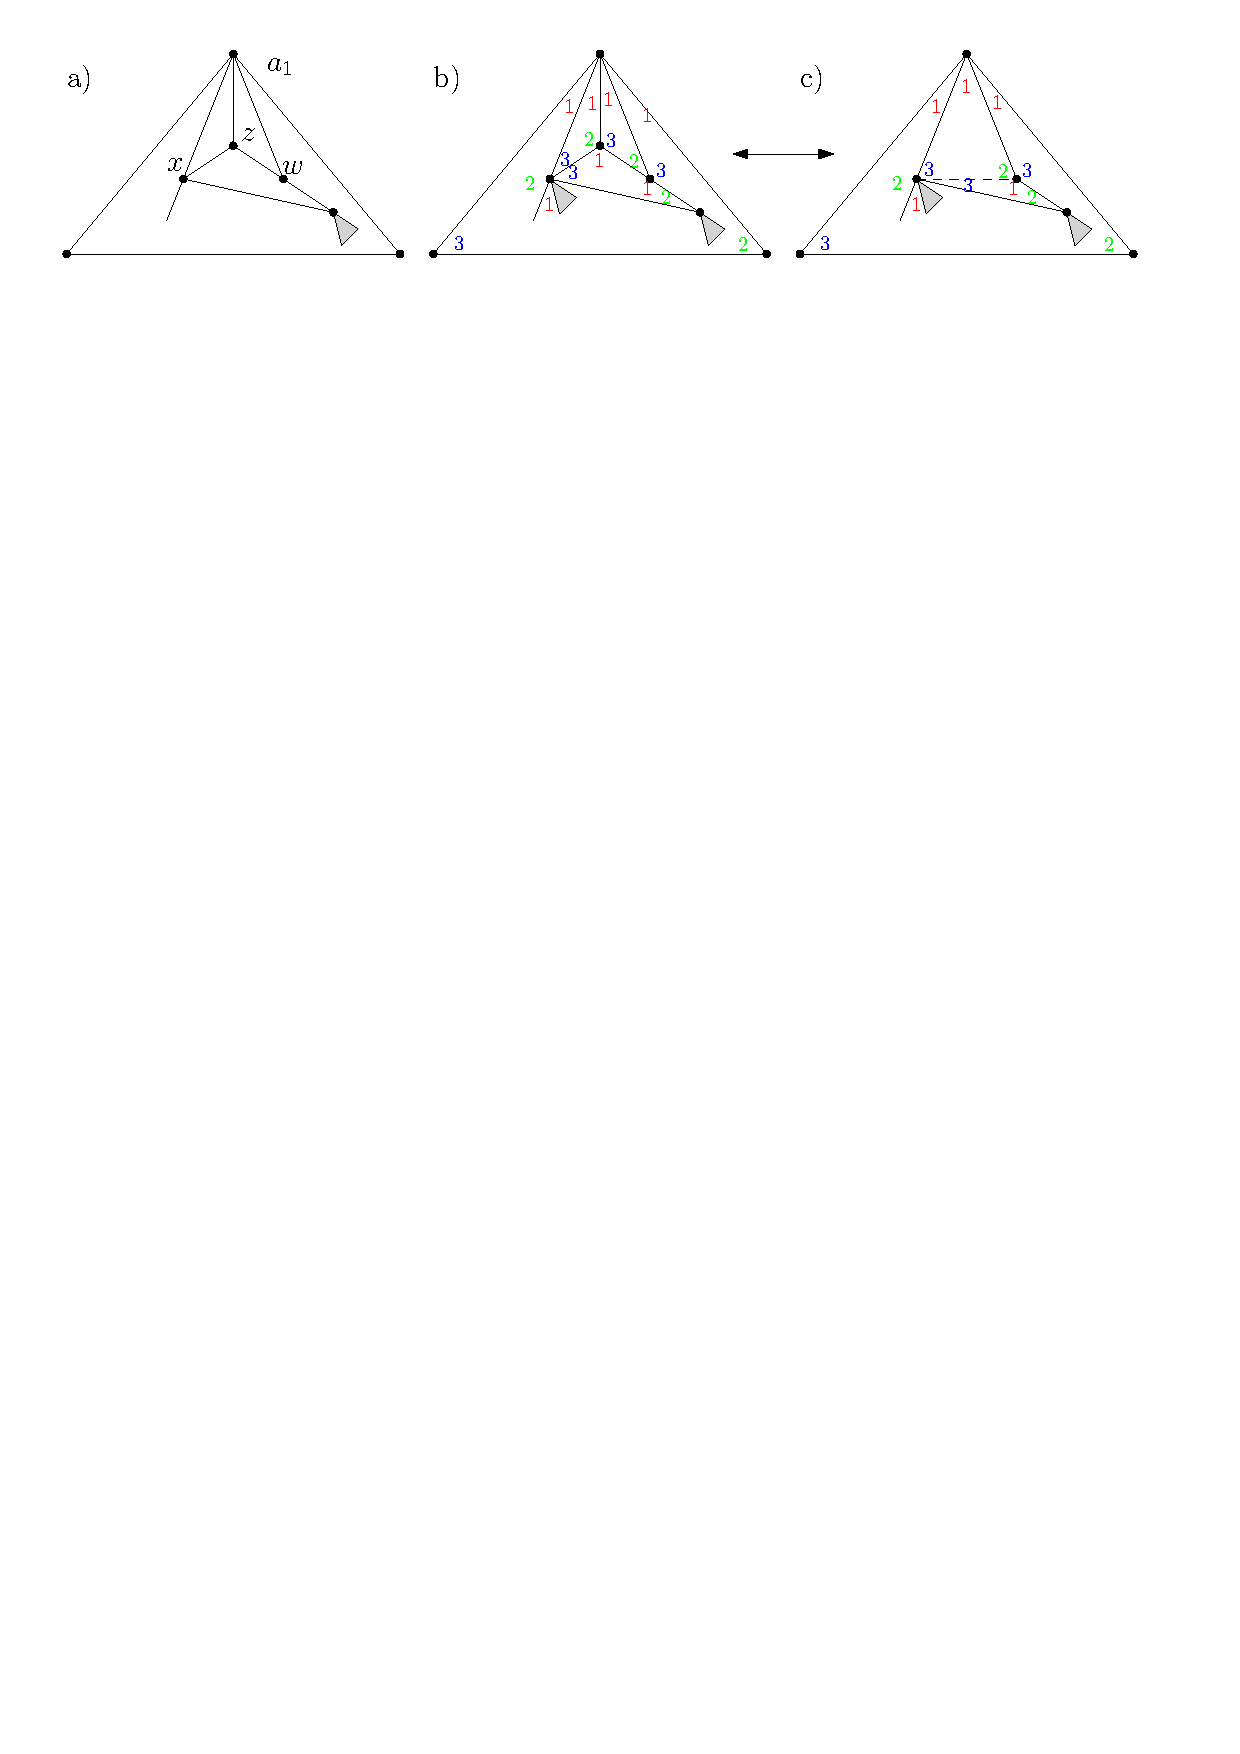
\includegraphics[width=1\textwidth]{lem5_5.pdf}
    	\caption{Das Löschen von $z$, falls $w$ dem Gebiet mit $z$ und $x$ zugewiesen ist oder wenn $w$ Grad 3 hat.}
    	\label{pic_lem5_5}
\end{figure}

Wir müssen nun $z$ wieder einfügen und zeigen, dass wir ein Ecken kompatibles Paar erhalten. Um $z$ wieder einzufügen, unterteilen wir die an $w$ neu eingefügte Kante, setzen $z$ auf ihr ein und verbinden $z$ mit dem verbliebenen Nachbarn in $G$ ($x$ bzw. $a_1$). Die Label an den Enden der unterteilen Kante ändern sich nicht. An $x$ bzw. $a_1$ übernehmen wir das Label, dass der jetzt geteilte Winkel in $G'$ hatte und fügen es links und rechts der neuen Kante ein. Die Label um $z$ sind eindeutig, weil $z$ Grad 3 hat und Nachbar einer Aufhängung ist. Wir fügen nun die Zuweisung von $w$ wieder ein, um $\phi$ zu erhalten. Der Winkel an $z$ neben der Zuweisung von $w$ erhält das gleiche Label wie diese. Somit haben die drei neuen Gebiete jeweils alle Label als Ecken und das erhaltene Schnyder Labeling $\sigma$ ist Ecken kompatibel zu $\phi$. Wieder kann $G$ kein Gegenbeispiel sein.

Nehmen wir nun an, dass $w$ dem Gebiet mit der Kante $(x,z)$ zugewiesen ist und mindestens Grad 4 hat. In diesem Fall muss der Vorgang von eben nicht zwangsläufig möglich sein. Betrachte Abbildung \ref{pic_lem5_5} c) und nehme an, dass $w$ mindestens Grad 4 hat. Dann können wir die Label nicht mit Sicherheit vorhersagen. Zum Beispiel könnten hier die Label um das Gebiet $f_{xwp}$ entgegen dem Uhrzeigersinn um eine Position verschoben sein und es würde trotzdem ein Schnyder Labeling vorliegen. Dann hätte aber $w$ als einziger Knoten das Label 2 und nach der Zuweisung von $w$ würde es keine Ecke mit Label 2 geben. Es läge also kein Ecken kompatibles Paar vor. Somit müssen wir unser Vorgehen, wie in Abbildung \ref{pic_lem5_6} illustriert, anpassen.

\begin{figure}[h]
	\centering
	  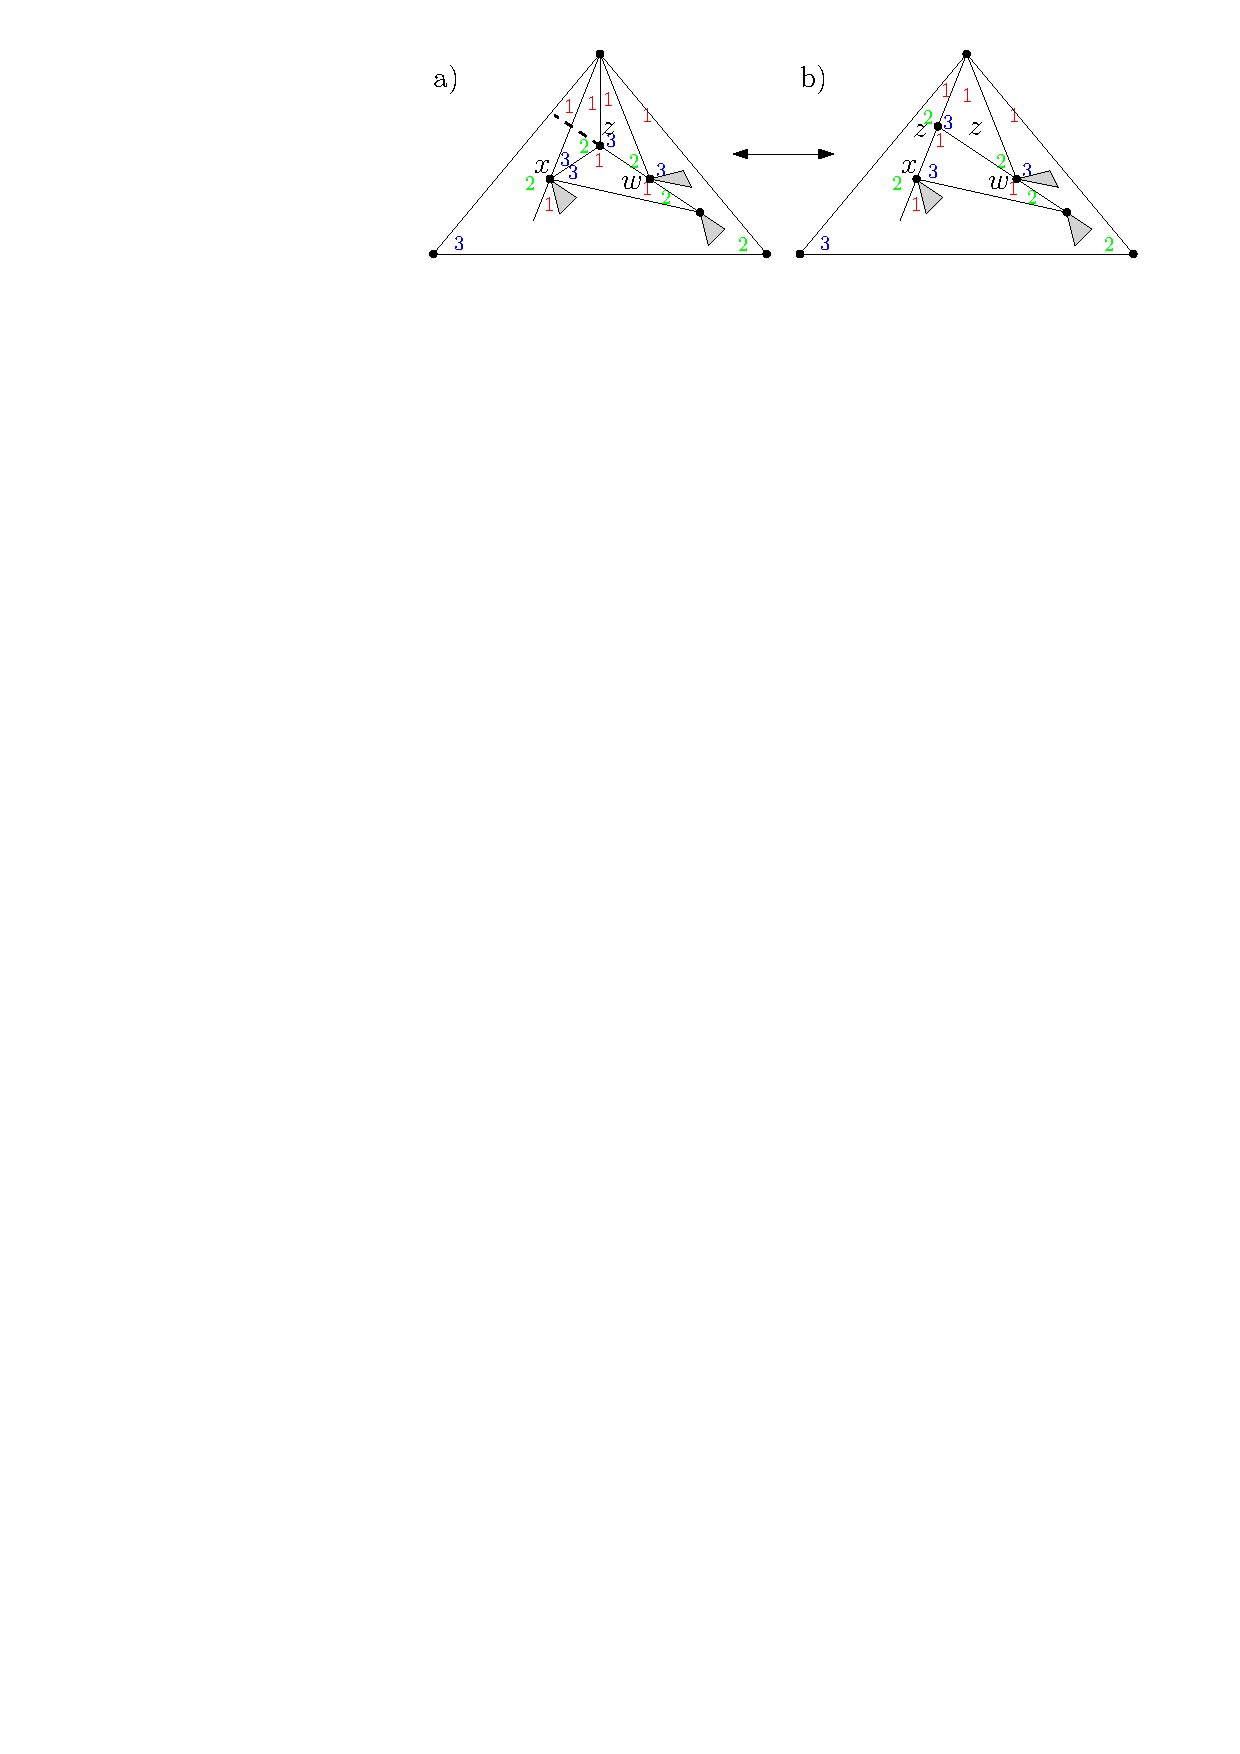
\includegraphics[width=0.66\textwidth]{lem5_6.pdf}
    	\caption{Das Löschen von $z$, falls $w$ mindestens Grad 4 hat. Wir verschieben den Knoten $z$ entlang der gestrichelten Geraden auf die Kante $(a_1,x)$ und erhalten so wieder eine SLTR.}
    	\label{pic_lem5_6}
\end{figure}

Wir werden $z$ nicht löschen, sondern auf der gestrichelten Geraden verschieben, bis wir die Kante $(a_1,x)$ erreichen und dann diese Kante löschen. Wir projizieren also $z$ in $\Delta$ auf die Gerade $(a_1,x)$. Dies ist möglich, da sich $z$ in $\Delta$ in der konvexen Hülle von $x,w$ und $a_1$ befindet und keine weiteren Knoten im Inneren dieser Hülle liegen. Wir erhalten somit den Graphen $G'$. Nach Konstruktion hat $G'$ eine SLTR und wir erhalten das FAA $\phi'$ durch Hinzufügen der Zuweisung von $z$ zu dem Gebiet, dem auch $x$ zugewiesen ist. $G'$ hat nun eine Kante weniger als $G$ und ist somit kein Gegenbeispiel. Sei $\sigma'$ das zu $\phi'$ Ecken kompatible Schnyder Labeling auf $G'$. Da wir in $\phi'$ eine Zuweisung hinzugefügt haben, erhalten wir ein Ecken kompatibles Paar auf $G$, da die einzig neuen Label im Gebiet $f_{a_1,z,x}$ eingefügt werden, das ein Dreieck ist. $G$ kann also kein Gegenbeispiel sein.

Dies beendet den Beweis für den Fall, dass $z$ Grad 3 hat.

\item[Fall 1c:] Als Folgerungen der Fälle 1a) und 1b) können wir annehmen, dass $z$ mindestens Grad 4 hat und keinem Gebiet zugeordnet ist, welches an $(x,z)$ grenzt. Somit können wir die Kante $(a_1,x)$ kontrahieren und die Kante $(x,z)$ löschen und erhalten $G'$ (siehe Abbildung \ref{pic_lem5_7}). Der Knoten $z$ hat nun in $G'$ mindestens Grad 3, weil er zuvor mindestens Grad 4 hatte. Wir erhalten das FAA $\phi'$ auf $G'$, indem wir die Zuweisung von $x$ aus $\phi$ löschen. 

Sei $\gamma'$ ein begrenzender Zykel in $G'$ und $\gamma$ der korrespondierende begrenzende Zykel in $G$. Wir müssen zeigen, dass $\gamma'$ drei kombinatorisch konvexe Ecken hat. Falls $x$ eine kombinatorisch konvexe Ecke von $\gamma$ ist, dann muss $a_1$ eine kombinatorisch konvexe Ecke von $\gamma'$ sein. Nehmen wir an, dass $z$ eine kombinatorisch konvexe Ecke von $\gamma$ und keine kombinatorisch konvexe Ecke von $\gamma'$ ist. Dann liegen alle Nachbarn von $z$, mit Ausnahme von $x$, auf dem Rand oder im Inneren von $\gamma$. Nehmen wir an, dass $\gamma'$ nur zwei kombinatorisch konvexe Ecken hat. Betrachte Abbildung \ref{pic_lem5_8} a). Sei $p$ der entgegen dem Uhrzeigersinn nächste Nachbar von $z$ nach $x$. Auf dem Pfad von $a_1$ zu $p$ muss mindestens ein Nachbar liegen, da $z$ mindestens Grad 4 hat. Falls alle Nachbarn von $z$ zwischen $p$ und $a_1$ auf dem Rand von $\gamma$ liegen und Gebieten außerhalb von $\gamma$ zugewiesen sind, existiert ein unterteilendes Dreieck in $G$ (siehe Abbildung \ref{pic_lem5_8} a). Falls der Pfad, wie in Abbildung \ref{pic_lem5_8} b) konkav ist, folgt dies nicht. Wir nennen $(a_1,x)$ nicht kontrahierbar und verweisen auf Fall 1d. Falls der Pfad anders herum konvex ist, dann liegt mindestens eine kombinatorisch konvexe Ecke $x'$ von $\gamma$ zwischen $p$ und $a_1$. Der Zykel $\gamma'$ hat somit die drei kombinatorisch konvexe Ecken $a_1,p$ und $x'$. 

\begin{figure}[h]
	\centering
	  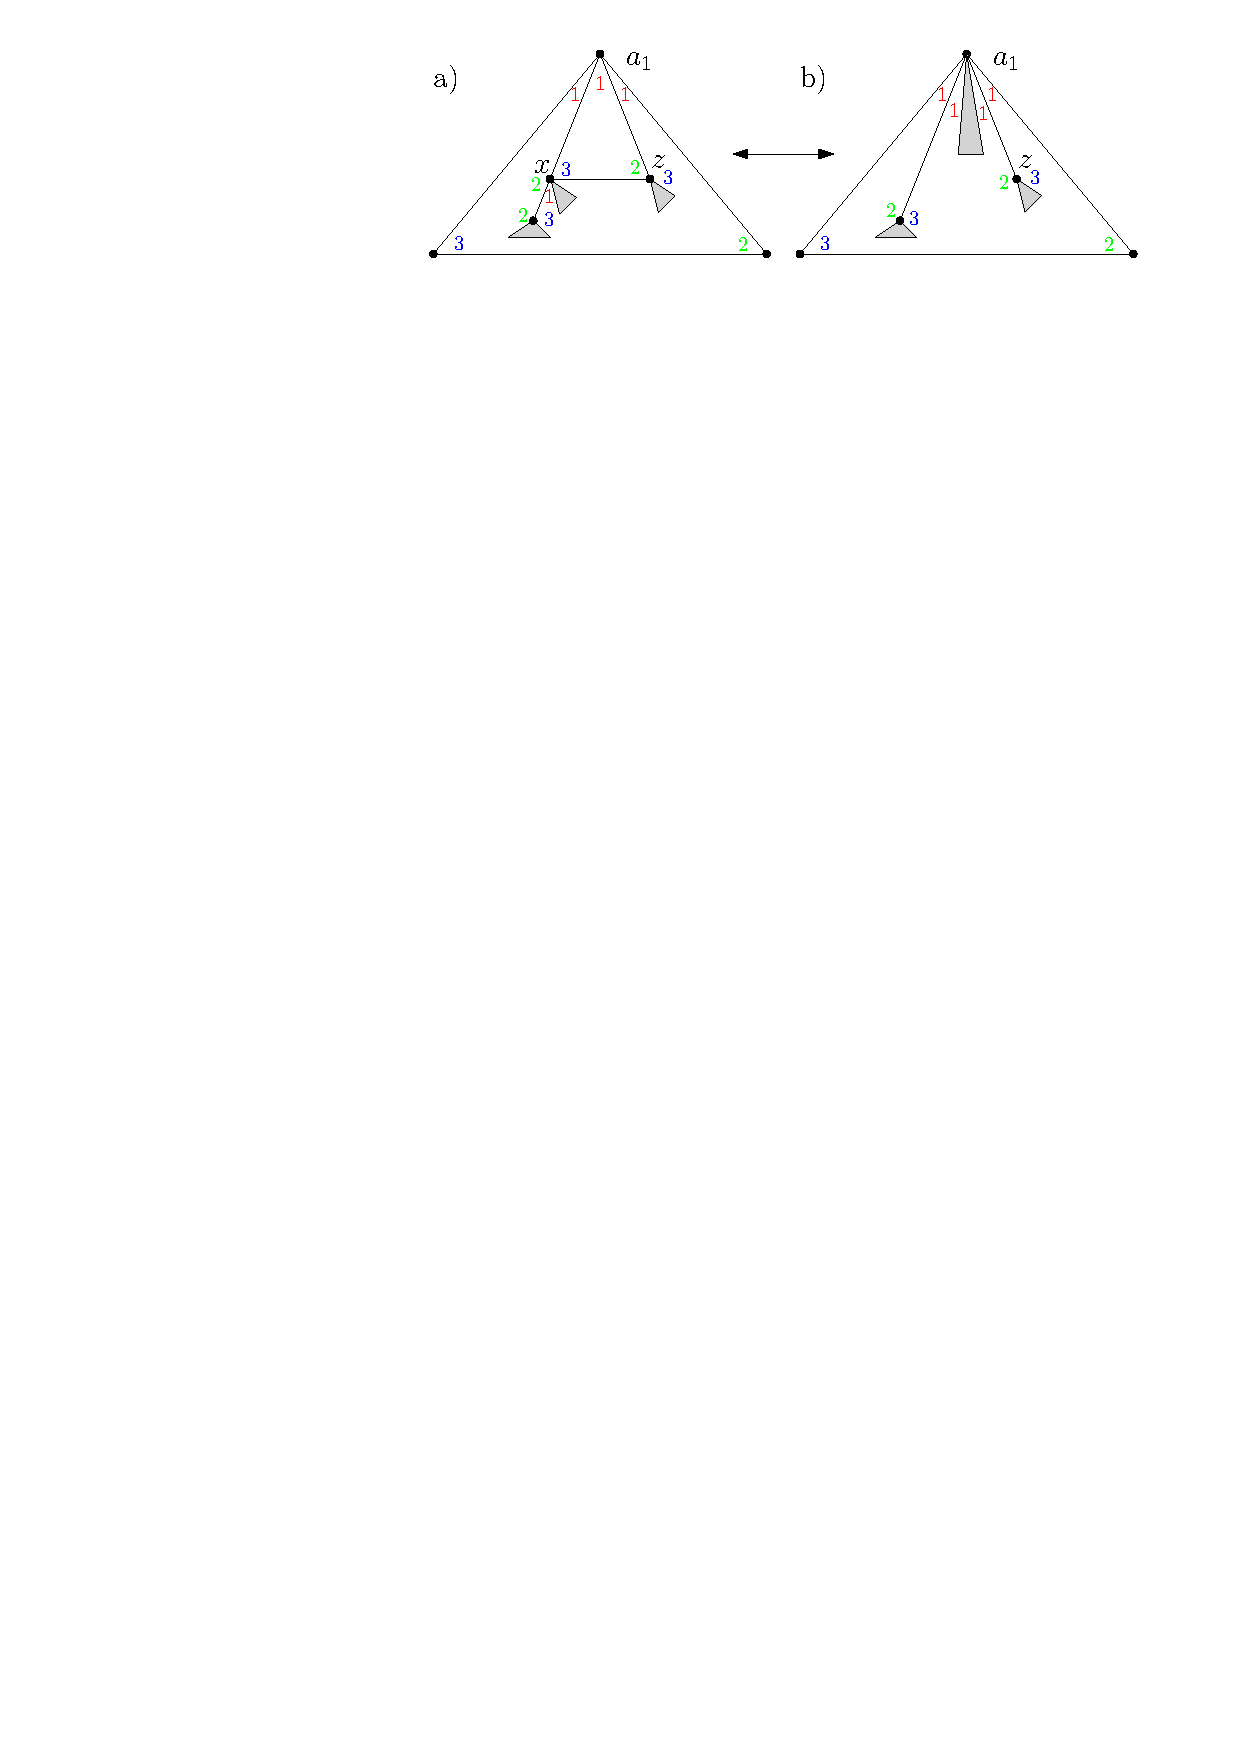
\includegraphics[width=0.66\textwidth]{lem5_7.pdf}
    	\caption{Falls $x$ dem Gebiet an $(a_1,x)$ zugewiesen ist, $(x,z)$ eine Kante ist und deg$(z)\geq 4$, kontrahieren wir die Kante $(a_1,x)$ und löschen $(x,z)$.}
    	\label{pic_lem5_7}
\end{figure}

Betrachten wir den Fall, dass kein begrenzender Zykel $\gamma$ in $G$ existiert, der $z$ als kombinatorisch konvexe Ecke hat. Weiter sei $z$ keine kombinatorisch konvexe Ecke von $\gamma'$. Somit ist $(a_1,x)$ kontrahierbar, jeder begrenzende Zykel in $G'$ hat mindestens drei kombinatorisch konvexe Ecken und $G'$ hat eine SLTR. Somit existiert ein Schnyder Labeling $\sigma'$, das Ecken kompatibel zu $\phi'$ ist (wir haben $\phi'$ durch Löschen der Zuweisung von $x$ erhalten). Wir können ein Schnyder Labeling $\sigma'$ zu $\sigma$ erweitern indem wir die Kontraktion einer Kante, die eine Aufhängung beinhaltet, umkehren (siehe Abbildung \ref{pic_lem5_8}). Die resultierenden Winkel Label sind eindeutig. Wir begründen die Ecken-Kompatibilität. Gebiet $f_{a_1,z,x}$ ist ein Dreieck und wir setzen beginnend bei $a_1$ die Label 1, 2 und 3 ein. Hinzu kommt, dass der von $\phi$ zugewiesene Winkel von $x$ nicht als einziger Label 2 hat. $G$ kann also kein Gegenbeispiel sein.

\begin{figure}[h]
\centering
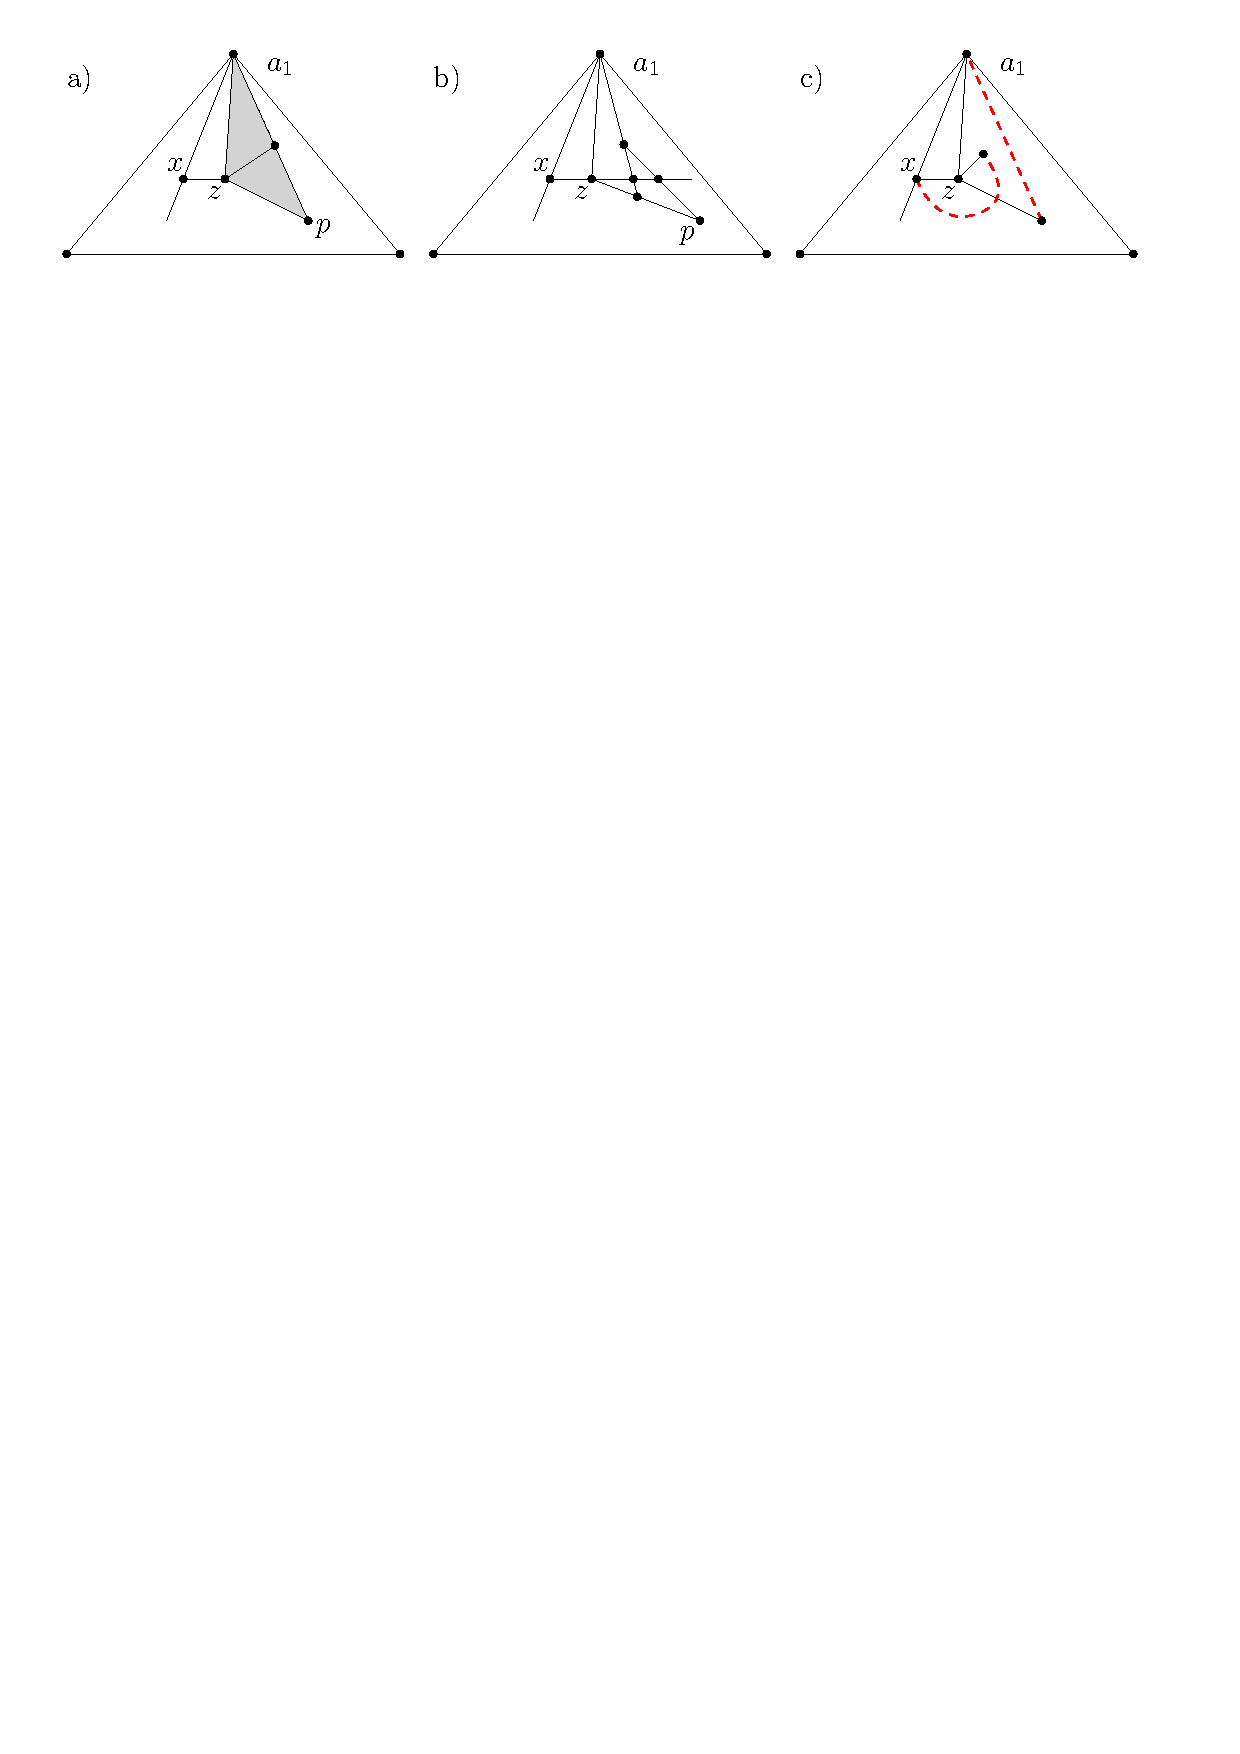
\includegraphics[width=1\textwidth]{lem5_8.pdf}
\caption{a) Falls der Pfad zwischen $a_1$ und $p$ entlang einer Gerade verläuft, dann existiert ein unterteilendes Dreieck. b) Wenn der Pfad konkav ist, dann können wir $(a_1,x)$ nicht kontrahieren. c) Nun muss jedoch der Nachbar von $z$, der im Uhrzeigersinn vor $x$ liegt, $a_1$ entlang der gestrichelten Gerade \glqq{sehen}\grqq{ } können, ohne von einem anderen Nachbarn von $z$ behindert zu werden. Somit kann dies für den im Uhrzeigersinn auf $a_1$ folgenden Nachbarn von $z$ und $x$ nicht gelten, wie die gestrichelte Kurve illustriert.}
\label{pic_lem5_8}
\end{figure}

\item[Fall 1d:] Aufgrund der bearbeiteten Fälle können wir annehmen, dass $z$ mindestens Grad 4 hat, keinem Gebiet zugeordnet ist, welches an $(x,z)$ grenzt und $(s_1,x)$ nicht kontrahierbar ist. Weil $(s_1,x)$ nicht kontrahierbar ist, muss ein begrenzender Pfad $\gamma$ in $G$ existieren, sodass $z$ auf dem Rand von $\gamma$ liegt, alle Nachbarn von $z$ ausser $x$ auf oder innerhalb von $\gamma$ liegen und $\gamma$ genau drei kombinatorisch konvexe Ecken hat, zu denen $z$ gehört. Betrachte Abbildung \ref{pic_lem5_8} b). Es liegen keine kombinatorisch konvexen Ecken von $\gamma$ auf dem Pfad zwischen $a_1$ und $p$. Somit wird die in Abbildung \ref{pic_lem5_8} c) eingezeichnete Gerade zwischen $p$ und $a_1$ nicht von der Nachbarschaft von $z$ unterbrochen. Der Knoten $p$ kann $s_1$ entlang dieser Gerade \glqq{sehen}\grqq{ } (an der Nachbarschaft vorbei). Da $z$ keinem Gebiet zugeordnet ist, welches an $(x,z)$ grenzt und keine kombinatorisch konvexe Ecke von $\gamma$ ist (die alle Nachbarn von $z$ ausser $x$ beinhaltet), kann $z$ nicht zugewiesen sein. 

Wir erstellen $G'$ durch Löschen der Kante $(a_1,z)$ aus $G$. Das FAA $\phi'$ folgt, indem wir die Zuweisung von $z$ zum Gebiet mit $a_1,x$ und $z$ zu $\phi$ hinzufügen (siehe Abbildung \ref{pic_lem5_9} b). Angenommen es existiert in $G'$ eine begrenzender Zykel $\gamma'$, der nur zwei kombinatorisch konvexe Ecke bezüglich $\phi'$ hat. Dann muss $z$ auf dem Rand von $\gamma'$ liegen und $z$ muss eine kombinatorisch konvexe Ecke des korrespondierenden Zykels $\gamma$ in $G$ sein. Falls nun $\gamma'$ alle Nachbarn von $z$ in $G'$ enthält, dann hat $\gamma$ mindestens vier kombinatorisch konvexe Ecken oder $z$ ist keine Ecke von $\gamma$, wie wir begründen werden. Wie in Abbildung \ref{pic_lem5_8} c) illustriert, kann der im Uhrzeigersinn erste Nachbar von $z$ nach $a_1$ den Knoten $x$ nicht \glqq{sehen}\grqq, weil ein Nachbar vor $x$ im Weg ist. Somit muss zwischen diesen beiden Nachbarn eine kombinatorisch konvexe Ecke von $\gamma$ liegen. Nehmen wir an, dass $\gamma'$ den zugewiesenen Winkel an $z$ in $G'$ einschließt. Weiter sei $z$ eine kombinatorisch konvexe Ecke des korrespondierenden Zykels $\gamma$. Dann muss $\gamma$ mindestens vier kombinatorisch konvexe Ecken in $G$ haben. Die beiden Ränder von $\gamma$ zwischen $a_1$ und $z$ müssen strikt konvex in der Zeichnung von $G$ sein und somit jeweils eine weitere kombinatorisch konvexe Ecke von $\gamma$ enthalten (vergleiche Abbildung \ref{pic_lem5_9} a).

Somit haben wir gezeigt, dass $G'$ eine SLTR hat. Erneut kann $G'$ kein Gegenbeispiel sein und wir erhalten ein Schnyder Labeling $\sigma'$, das Ecken kompatibel zu $\phi'$ ist. Wir können dies, wie in Abbildung \ref{pic_lem5_9} b) zu sehen ist, zu einem Schnyder Labeling $\sigma$ von $G$ erweitern, das Ecken kompatibel zu $\phi$ ist, da wir kein Label an einer Zuweisung aus $\phi$ ändern. Somit kann $G$ kein Gegenbeispiel sein.

Dies beendet den Beweis für den Fall, das $x$ und $z$ Nachbarn sind.

\begin{figure}[h]
\centering
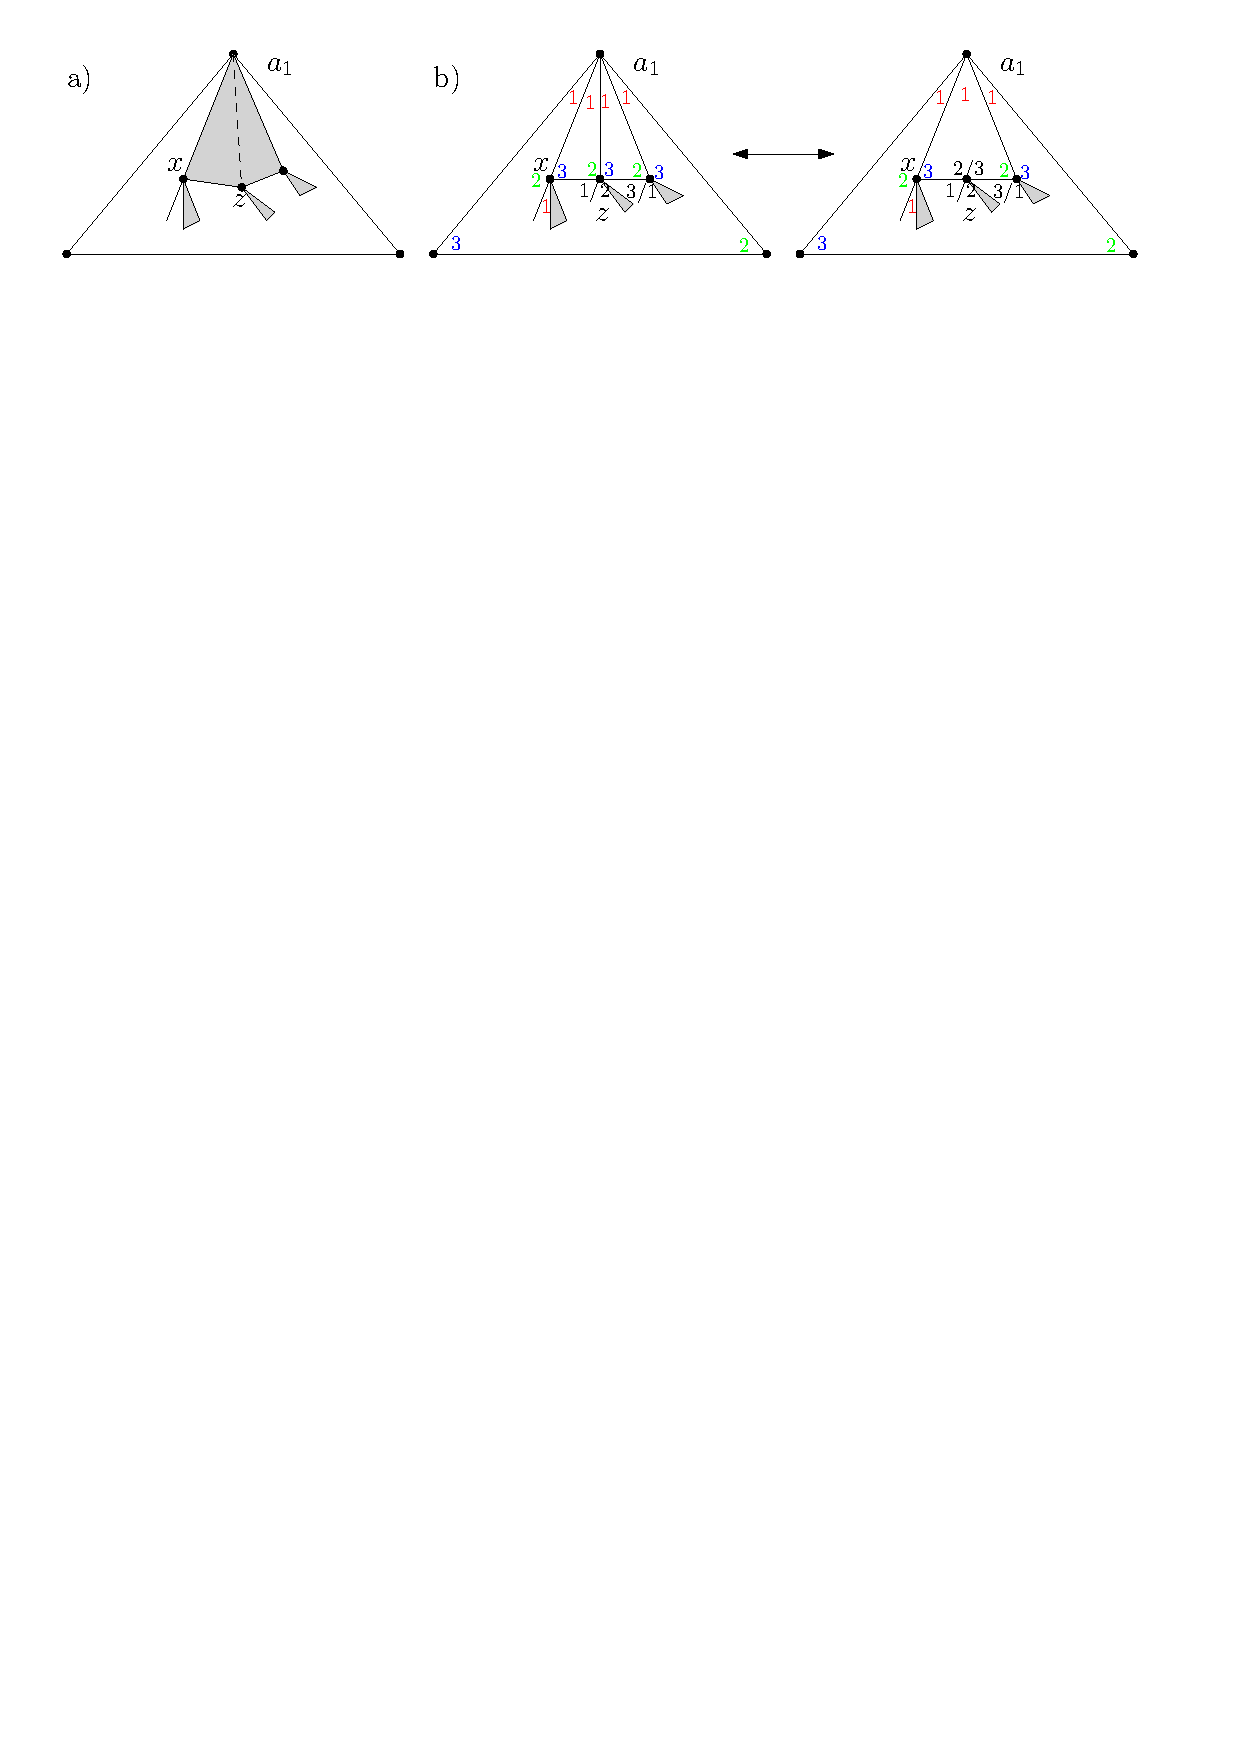
\includegraphics[width=1\textwidth]{lem5_9.pdf}
\caption{a) Falls $z$ eine kombinatorisch konvexe Ecke des begrenzenden Zykels $\gamma$ (um den grauen Teilgraphen) ist, dann hat $\gamma$ mindestens vier kombinatorisch konvexe Ecken, da die Pfade von $a_1$ zu $z$ auf beiden strikt Seiten konvex sind. b) Löschen der Kante $(a_1,z)$. }
\label{pic_lem5_9}
\end{figure}

\item[Fall 2:] Seien nun $x$ und $z$ nicht benachbart, dann muss mindestens ein Knoten auf der Gerade zwischen ihnen liegen. Wir nennen diesen Knoten $p$. Der Knoten $p$ muss dem Gebiet mit den Ecken $a_1,z,x$ zugewiesen sein (vergleiche Abbildung \ref{pic_lem5_10}). Wir wählen $p$, sodass die Kante $(x,p)$ existiert. Wir erhalten $G'$ durch die Kontraktion der Kante $(a_1,x)$. Das FAA $\phi'$ von $G'$ folgt durch Löschen der Zuweisungen von $x$ und $p$ aus $\phi$.

\begin{figure}[h]
\centering
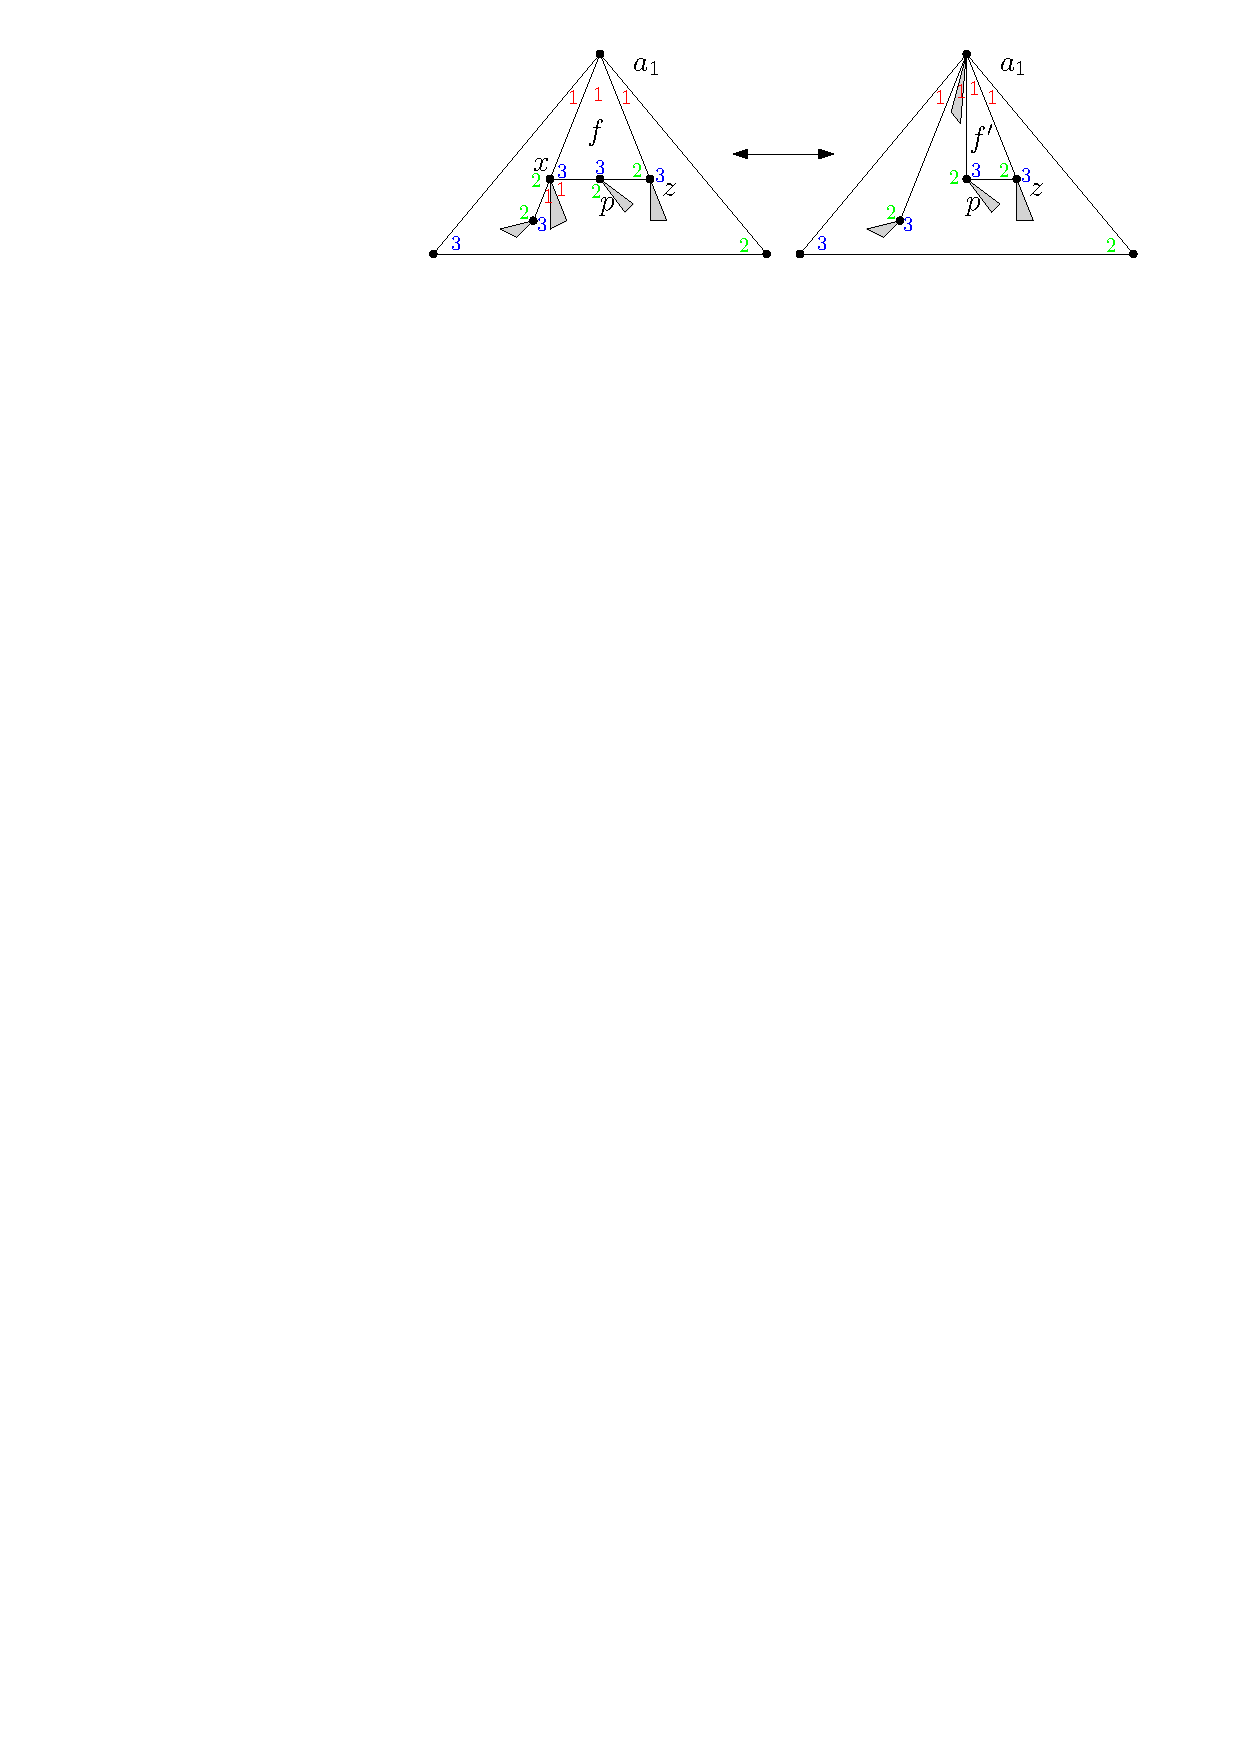
\includegraphics[width=0.66\textwidth]{lem5_10.pdf}
\caption{Kontraktion der Kante $(a_1,x)$, wenn $x$ einem Gebiet an $(a_1,x)$ zugeordnet ist und $x$ und $z$ nicht benachbart sind.}
\label{pic_lem5_10}
\end{figure}

Wir betrachten einen begrenzende Zykel $\gamma$ in $G'$ und seinen korrespondierenden begrenzenden Zykel $\gamma$ in $G$. Falls $x$ eine kombinatorisch konvexe Ecke vom $\gamma$ ist, dann sind $p$ oder $a_1$ die korrespondierende kombinatorisch konvexe Ecke von $\gamma'$. Beachte, dass wir die Zuweisung von $p$ geändert haben. Falls $p$ eine kombinatorisch konvexe Ecke eines korrespondierenden Zykels $\gamma$ in $G$ ist, dann muss $p$ in $G$ einen Nachbar außerhalb von $\gamma$ besitzen. Da sich der Grad von $p$ in $G'$ nicht ändert, muss dieser Nachbar auch außerhalb von $\gamma'$ in $G'$ liegen. Es folgt, dass $p$ eine kombinatorisch konvexe Ecke von $\gamma'$ ist, da $p$ nicht zugewiesen ist. Somit hat jeder begrenzende Zykel in $G'$ mindestens drei kombinatorisch konvexe Ecken und wir haben gezeigt, dass $G'$ eine SLTR hat, die von $\phi'$ induziert wird.

Der Graph $G'$ hat einen Knoten weniger als $G$ und kann somit kein Gegenbeispiel sein. Sei nun $\sigma'$ das zu $\phi'$ Ecken kompatible Schnyder Labeling von $G'$. Wir müssen nun zeigen, dass im Gebiet $f$ mit den Ecken $a_1,z$ und $x$, in dem auch $p$ liegt, jede Ecke ein anderes Label hat. Sei $f'$ das zu $f$ korrespondierende Gebiet in $G'$ (siehe Abbildung \ref{pic_lem5_10}). Im Schnyder Labeling $\sigma'$ hat der Winkel an $p$ das Label 3 in $f'$, weil er auf der rechten Seite einer Kante zur Aufhängung mit Label 1 liegt. Der Winkel an $x$ in $f$ hat aus dem gleichen Grund ebenfalls Label 3 in $\sigma$. Somit haben weder $p$ noch $x$ in ihren von $\phi$ zugewiesenen Gebieten Label in $\sigma$, die in diesen Gebieten nur einmal vorkommen. Da $\phi'$ Ecken kompatibel zu $\sigma'$ ist, bilden auch $\sigma$ und $\phi$ ein Ecken kompatibles Paar zur SLTR $\Delta$ von $G$.
\end{description}
Wir haben somit für alle aufgelisteten Fälle einen Widerspruch zur Annahme erhalten, dass $G$ ein minimales Gegenbeispiel ist. Dies beendet den Beweis.
\end{proof}

In einem letzten Lemma werden wir nun zeigen, dass kein Gegenbeispiel $G$ existieren kann, das eine SLTR (mit dem induzierten FAA $\phi$) zulässt, auf dem aber kein Schnyder Labeling $\sigma$ existiert, welches Ecken kompatibel zu $\phi$ ist.

\begin{lemma}\label{lem6}
Sei G ein ebener, intern-3-zusammenhängender Graph mit den Aufhängungen $\{a_1,a_2,a_3\}$, der eine SLTR besitzt. Sei $\phi$ das von dieser SLTR induzierte FAA. Dann existiert ein Schnyder Labeling $\sigma$ von $G$, sodass $\sigma$ und $\phi$ ein Ecken kompatibles Paar bilden.
\end{lemma}

\begin{proof}
Angenommen das Lemma gilt nicht. Sei $G$ ein minimales Gegenbeispiel, wie zuvor mit der minimalen Anzahl an Knoten und unter diesen mit der minimalen Anzahl an Kanten. Sei $\Delta$ eine SLTR von $G$ mit den Aufhängungen $a_1,a_2,a_3$ und $\phi$ das induzierte FAA. Wir wollen wieder zu einem Widersprich gelangen, indem wir einen kleineren Graphen $G'$ konstruieren, sodass die folgenden Punkte erfüllt sind.
\begin{itemize}
\item $G'$ besitzt ein FAA $\phi'$, welches von $\phi$ induziert wird.
\item Das kompatible Paar $(\sigma',\phi')$ von $G'$ induziert ein Schnyder Labeling von $G$.
\item Das so erzeugte Schnyder Labeling $\sigma$ ist Ecken kompatibel zu $\phi$.
\end{itemize}
Diese Aussagen zusammen erzeugen einen Widerspruch zur Annahme, dass $G$ ein Gegenbeispiel ist. Wir halten einige Beobachtungen aus den vorherigen Lemmata fest.
\begin{itemize}
\item [B1] $\Delta$ hat kein unterteilendes Dreieck.
\item [B2] $\Delta$ hat kein teilendes Segment und somit keine Aufhängung von Grad 2.
\item [B3] Kein Nachbar $x_i$ einer Aufhängung $a_i$ kann einem Gebiet zugeordnet sein, zu dessen Rand die Kante $(a_i,x_i)$ gehört. Somit bilden die Aufhängungen von $\Delta$ ein Dreieck.
\end{itemize}

Aus B3 folgt, dass sowohl das äußere Gebiet als auch seine drei benachbarten Gebiete (echte) Dreiecke\footnote{Sie enthalten nur jeweils ihre drei Ecken als Knoten.} sind (siehe Abbildung \ref{pic_lem6_1} a). Wir werden sehen, dass der dritte Knoten in einem der inneren Dreiecke eine wichtige Rolle spielt. Wir bezeichnen den dritten Knoten im Dreieck, das $a_i$ und $a_{i+1}$ enthält, mit $q_i$ (oder einfach nur $q$).

Der Beweis läuft in drei Schritten. Wir zeigen zuerst, dass in einem minimalen Gegenbeispiel $\Delta$ jedes $q_i$ einem angrenzenden Gebiet zugeordnet sein muss (und in diesem einen flachen Winkel hat). Als nächstes zeigen wir, dass wir aus $G$ einen Graphen $G'$ erzeugen können, der einen zugewiesenen Knoten $q'$ auf einer Kante $(a_i,q')$ besitzt und erhalten einen Widerspruch zu B3. Zuletzt zeigen wir, dass wir aus einem Schnyder Labeling $\sigma'$ von $G'$ ein Labeling $\sigma$ von $G$ erzeugen können, sodass aus der Ecken Kompatibilität von $\sigma'$ und $\phi'$ auch Kompatibilität von $\sigma$ und $\phi$ folgt.

\begin{figure}
	\centering
	  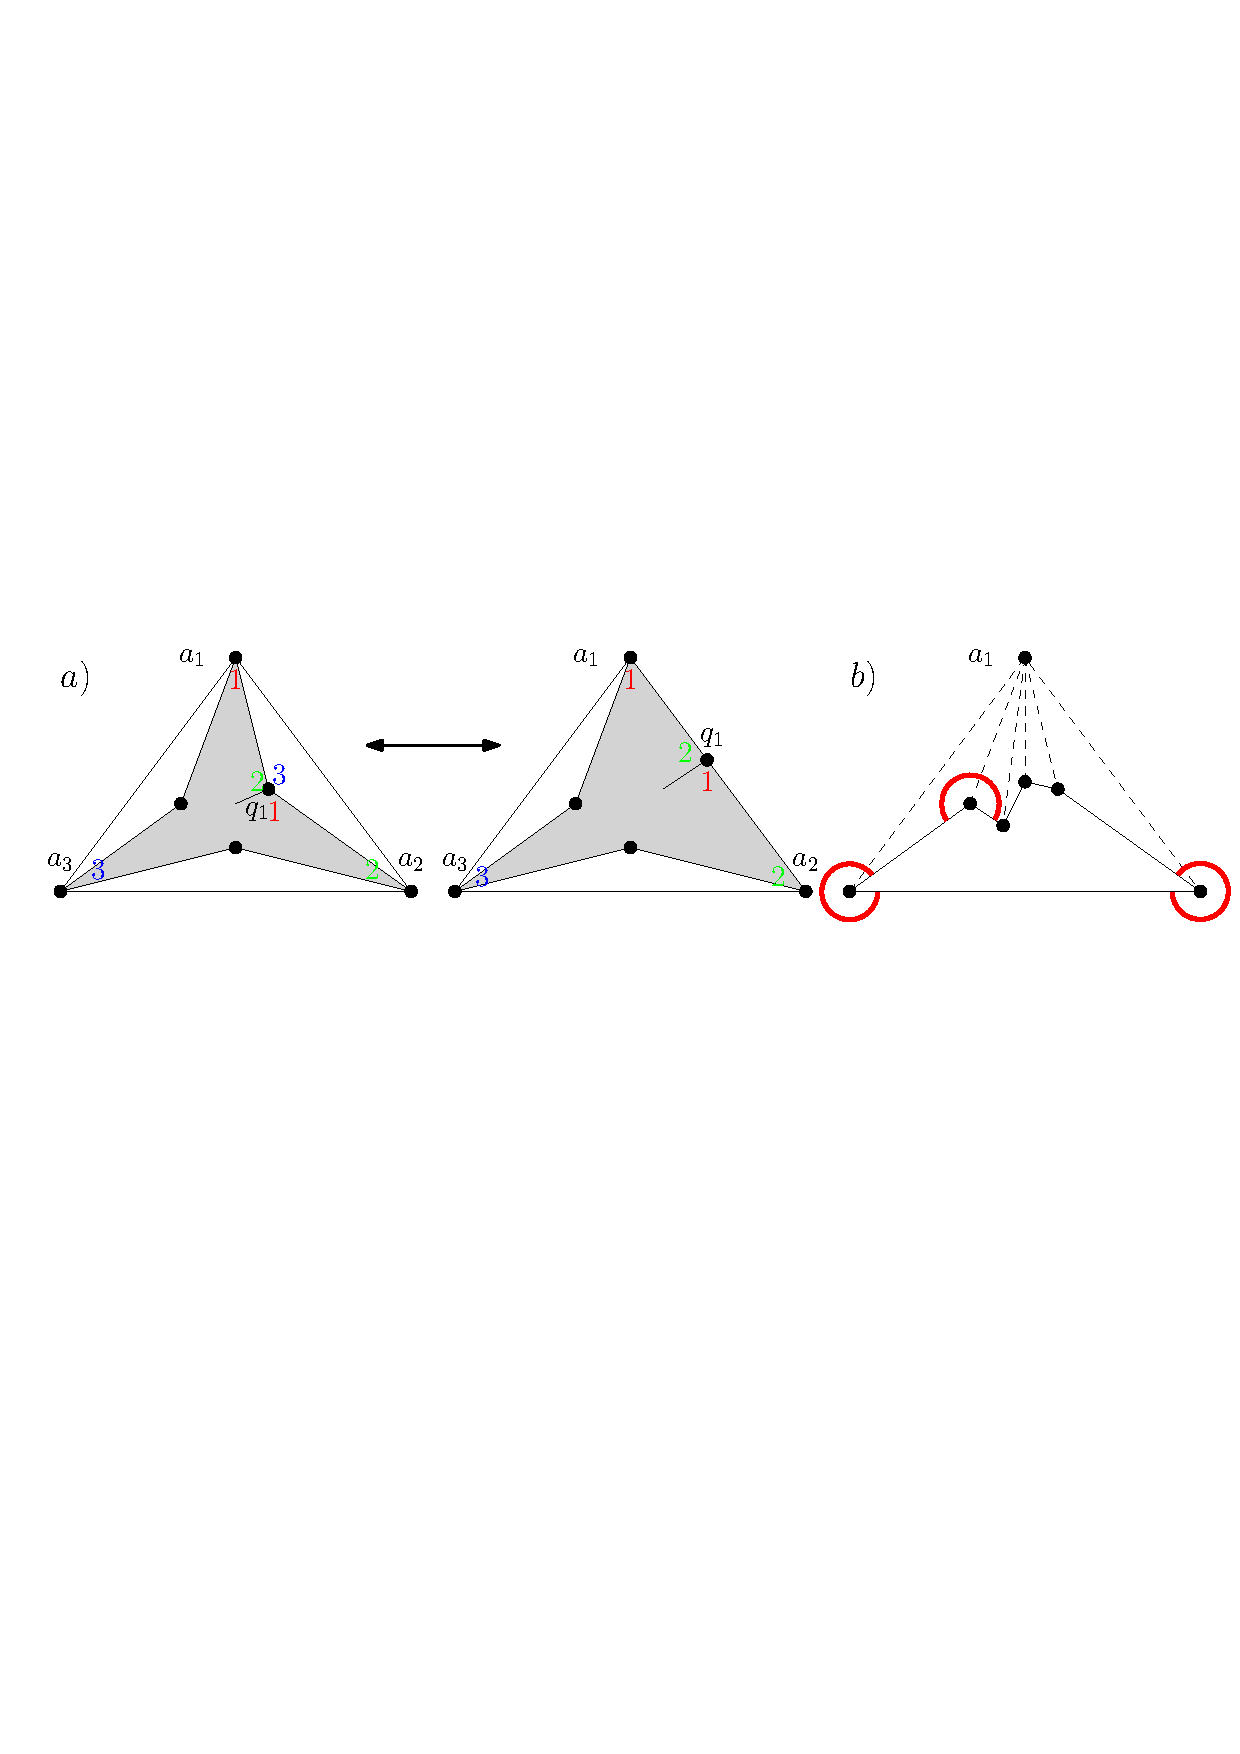
\includegraphics[width=1\textwidth]{lem6_1.pdf}
    	\caption{a) Die Erstellung eines Graphen $G'$ mit weniger Kanten. b) Das Löschen einer Aufhängung resultiert in einem Graphen mit mindestens drei Außenwinkeln $\geq \pi$.}
    	\label{pic_lem6_1}
\end{figure}

Sei $f$ das von $a_1,a_2$ und $q_1$ gebildete Dreieck (siehe Abbildung \ref{pic_lem6_1} a). Angenommen $q_1$ wird von $\phi$ nicht zugeordnet. Entferne die Kante $(a_1,a_2)$ und weise $q_1$ in dem äußeren Gebiet zu, um $G'$ und $\sigma'$ zu erhalten. Kein begrenzender Zykel enthält den neu zugewiesenen Winkel an $q$ in seinem Inneren. Falls $a_1$ und $a_2$ auf einem begrenzenden Zykel $\gamma'$ liegen, dann ist $q$ keine kombinatorisch konvexe Ecke des korrespondierenden Zykels $\gamma$ in $G$, sondern muss in seinem Inneren liegen (sonst wäre $\gamma'$ von einem Pfad induziert). Somit sind die kombinatorisch konvexen Ecken von $\gamma$ auch kombinatorisch konvexen Ecken von $\gamma'$. Da Zykel, die $q_1$ nicht enthalten, keine Ecken verlieren, hat jeder begrenzende Zykel in $G'$ mindestens drei kombinatorisch konvexe Ecken. Somit hat $G'$ ein SLTR $\Delta'$ und die gerade Winkel werden von $\phi'$ induziert. Nun ist $G'$ ein Graph mit weniger Kanten als $G$ und somit kein Gegenbeispiel. Wir erhalten also ein Ecken kompatibles Paar $(\sigma',\phi')$. Wir können dies wie in Abbildung \ref{pic_lem6_1} a) zu einem Paar für $G$ erweitern, indem wir die Zuweisung für $q_1$ löschen und im Dreieck $q_1,a_2,a_1$ die passenden Label einfügen.

Nehmen wir also an, dass jedes der $q_i$ in einem Gebiet einen flachen Winkel hat, also von $\phi$ einem Gebiet zugeordnet wird. Jede Aufhängung $a_i$ muss mindestens einen Nachbarn $x_i$ haben, der nicht zugeordnet ist. Nach Lemma \ref{lem5} kann kein Nachbar einer Aufhängung einem Gebiet an dieser Aufhängung zugewiesen sein. Somit würde ein Widerspruch zur Tatsache entstehen, dass $G\backslash \{a_1\}$ drei konkave Außenwinkel hat (siehe Abbildung \ref{pic_lem6_1} b). Der Knoten mit Winkel $\geq \pi$, der keine Aufhängung ist, kann nicht zugeordnet sein. Sei nun ohne Beschränkung der Allgemeinheit $q$ der gemeinsame Nachbar von $a_1$ und $a_2$. Der Knoten $p_k$ sei der im Uhrzeigersinn von $q$ ausgehend erste Nachbar von $a_1$, der nicht zugewiesen ist. In Abbildung \ref{pic_lem6_2} ist dies $p_3$.

Wir werden einen Graphen $G'$ (mit der gleichen Anzahl an Knoten und weniger Kanten) aus $G$ erstellen. In diesem Graphen ist $p_k$ einem Gebiet zugeordnet, auf dessen Rand die Kante $(a_1,p_k)$ liegt. Nach Lemma \ref{lem5} muss somit ein Schnyder Labeling $\sigma'$ existieren, dass Ecken kompatibel mit dem induzierten FAA $\phi'$ von $G'$ ist. Wir können aus $\sigma'$ ein Schnyder Labeling $\sigma$ für $G$ bauen, dass kompatibel zu $\phi$ ist.

Sei $N_{a_1} = \{q,p_1,\ldots,p_k,\ldots,p_l,a_3,a_2\}$ die Menge der Nachbarn von $a_1$, wobei wir mit $q$ beginnen und im Uhrzeigersinn fortfahren. Durch Löschen der Kante $(a_1,q)$ und Einfügen der Kante $(a_2,p_1)$ erhalten wir einen neuen Graphen $G_1$. Wir nennen den durchgeführten Kantenwechsel, um $G_1$ zu erhalten, (nach dem Englischen) einen \textit{Flip}. Nun lässt $G_1$ die SLTR $\Delta_1$ zu. Die vier Knoten $a_1,a_2,q$ und $p$ bilden in $\Delta$ ein konvexes Viereck\footnote{Auf der Geraden zwischen $q$ und $p_1$ können sich zusätzliche Knoten befinden, doch dies spielt für unsere Argumentation keine Rolle.} mit nur einer Diagonalen im Inneren (vergleiche Abbildung \ref{pic_lem6_2} a, b). Die durch den Flip, also das Wechseln der Diagonalen, erhaltene Zeichnung $\Delta_1$ ist somit ebenfalls eine SLTR. Falls $p_1$ zugewiesen ist, wiederholen wir den Schritt (siehe Abbildung \ref{pic_lem6_2} c). Wir führen diesen Schritt nur so oft durch, bis wir bei $p_k$ angekommen sind, dem ersten nicht zugewiesenen Nachbarn von $a_1$. Wir führen einen letzten Flip im konvexen Viereck mit den Ecken $a_1,a_2,p_{k-1},p_k$ durch. Wir ersetzen also die Diagonale $(a_1,p_{k-1})$ durch $(a_2,p_{k})$. Nach jedem Flip erhalten wir ein SLTR $\Delta_i$ und ein indiziertes Gutes-FAA $\phi_i$ von $G_i$. Somit ist $\phi_k$ ein Gutes-FAA.

\begin{figure}
	\centering
	  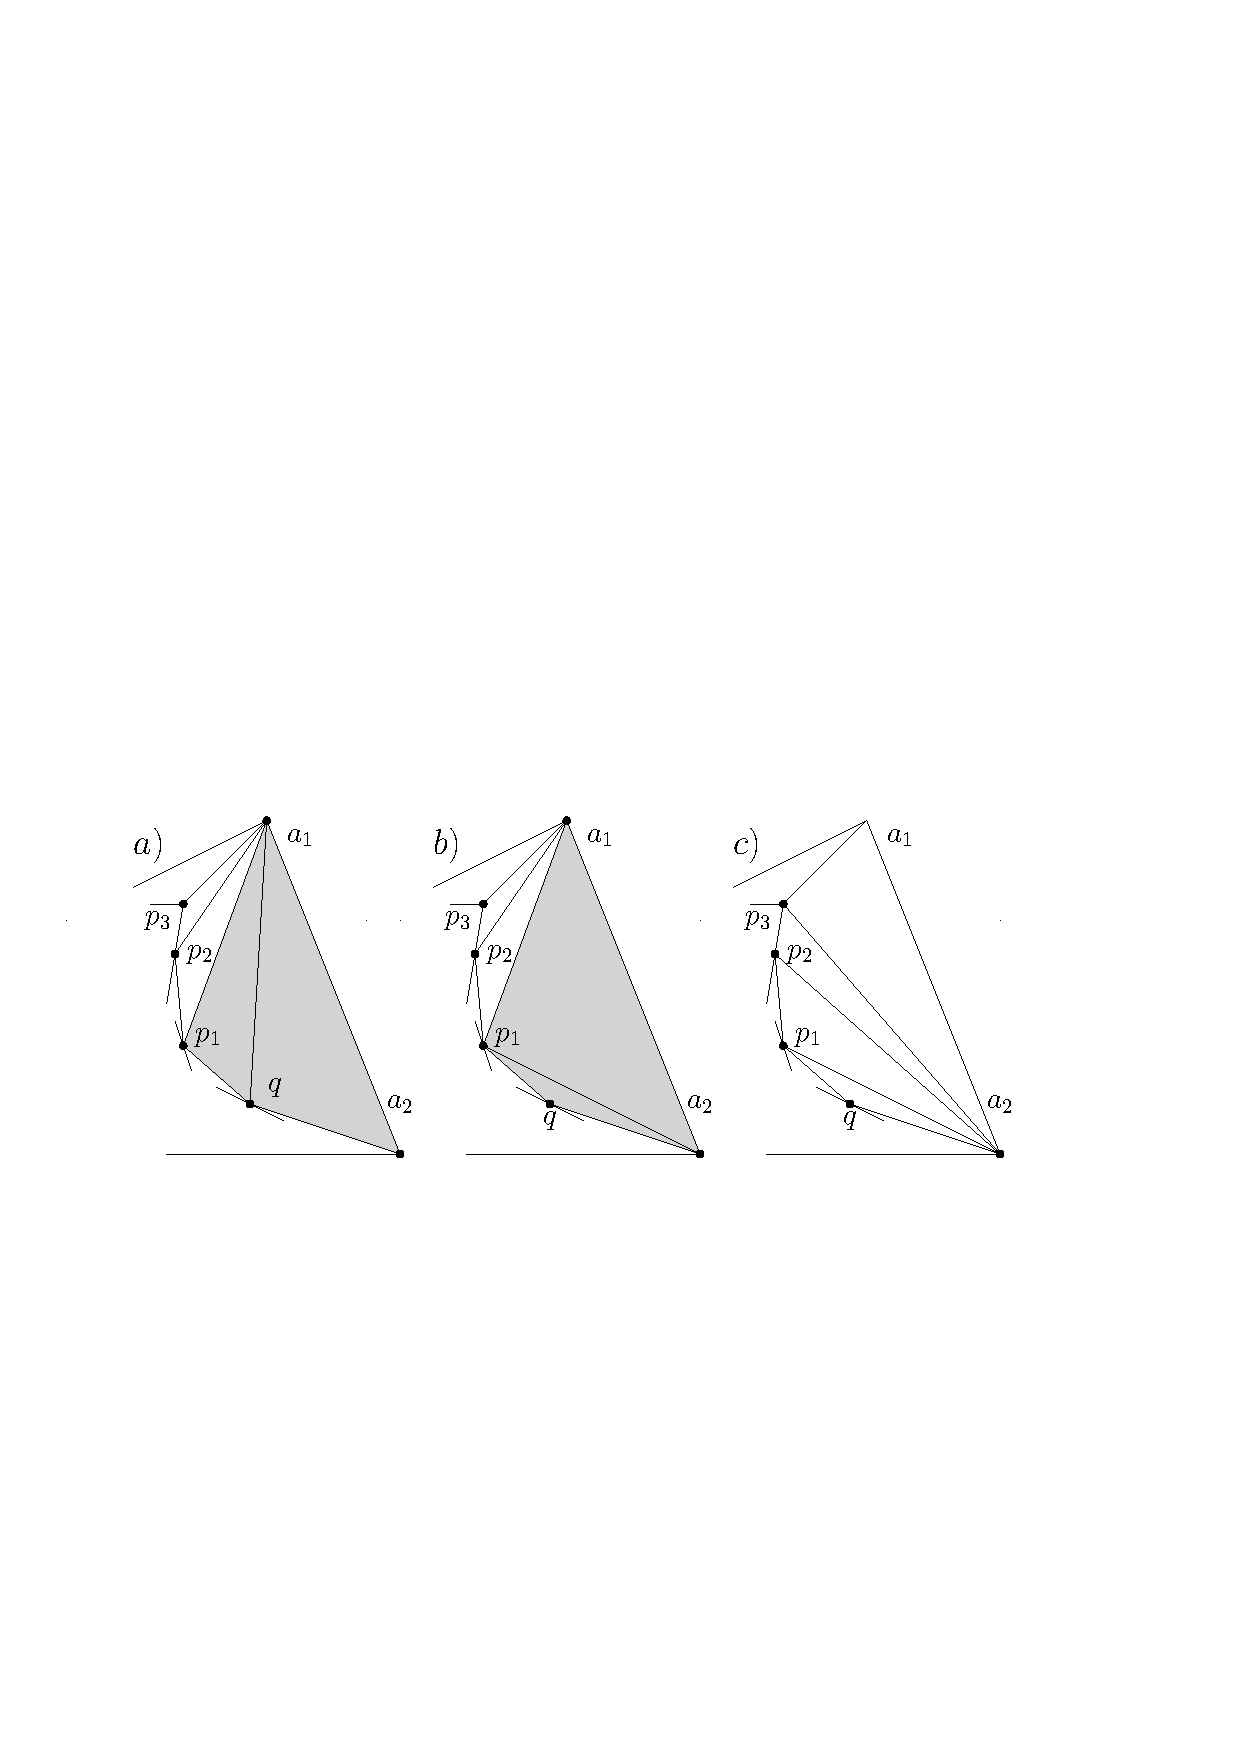
\includegraphics[width=1\textwidth]{lem6_2.pdf}
    	\caption{Das schrittweise Flippen von Kanten.}
    	\label{pic_lem6_2}
\end{figure}

Um nun den Graphen $G'$ zu erhalten, löschen wir die im letzten Flip hinzugefügte Kante $(a_2,p_{k})$ (siehe Abbildung \ref{pic_lem6_3} b). $G'$ hat somit eine Kante weniger als $G$. $p_k$ ist in $\phi_k$ nicht zugewiesen. Wir konstruieren $\phi'$ durch Hinzufügen der Zuweisung von $p_k$ zum Gebiet $a_1,a_2,p_{k-1},p_k$ zu $\phi$(siehe Abbildung \ref{pic_lem6_3} a). Das so konstruierte $\phi'$ ist ein FAA von $G'$. Wir zeigen als Nächstes, dass es sich bei $\phi'$ um ein Gutes-FAA handelt.

Betrachten wir einen beliebigen begrenzenden Zykel $\gamma'$ in $G'$ und sei $\gamma_k$ der korrespondierende Zykel in $G_k$. Wir müssen wieder zeigen, dass jeder Zykel mindestens drei kombinatorisch konvexe Ecken hat. Falls $p_k$ nicht auf dem Rand von $\gamma'$ liegt, folgt sofort, dass beide Zykel die selben kombinatorisch konvexen Ecken haben (und somit beide mindestens drei). Betrachten wir also den Fall, dass $p_k$ auf dem Rand von $\gamma'$ liegt. Falls $\gamma'$ nur einen Teil der Nachbarschaft von $p_k$ beinhaltet und der zugewiesene Winkel an $p_k$ nicht im Inneren von $\gamma'$ liegt, dann ist $p_k$ eine kombinatorisch konvexe Ecke von $\gamma_k$ und somit auch von $\gamma'$. Sei also $p_k$ keine kombinatorisch konvexe Ecke von $\gamma'$. Falls der zugewiesene Winkel an $p_k$ im Inneren von $\gamma'$ liegt, aber $\gamma'$ nicht alle Nachbarn von $p_k$ enthält, muss $\gamma_k$ mindestens vier kombinatorisch konvexe Ecken besitzen. Die ersten drei sind $a_1,a_2$ und $p_k$ und die vierte befindet sich auf dem Teil $R$ von $\gamma'$ zwischen $p_k$ und $a_2$\footnote{Diese Ecke muss existieren, da der begrenzende Zykel $\tilde{\gamma}$, der sich aus $R$ und der Kante $(a_2,p_k)$ bildet, mindestens drei kombinatorisch konvexe Ecken in $G_k$ hat.}. Somit hat $\gamma'$ mindestens drei kombinatorisch konvexe Ecken. Betrachte den Fall, dass $\gamma'$ alle Nachbarn von $p_k$ beinhaltet, aber der zugewiesene Winkel nicht im Inneren von $\gamma'$ liegt. In der SLTR $\Delta_k$ ist der Außenwinkel von $\gamma_k$ am Knoten $p_k$ somit nicht grösser als $\pi$ und $\gamma_k$ muss drei andere (kombinatorisch konvexe) Ecken haben. Diese sind auch kombinatorisch konvexe Ecken von $\gamma'$. Somit hat jeder begrenzende Zykel $\gamma'$ in $G'$ mindestens drei kombinatorisch konvexe Ecken und es folgt, dass $\phi'$ ein Gutes-FAA ist.

Da $G'$ die gleiche Anzahl an Knoten und weniger Kanten hat als $G$, kann er kein Gegenbeispiel sein. Es existiert also ein Schnyder Labeling $\sigma'$, das Ecken kompatibel zu $\phi'$ ist. Es bleibt zu zeigen, dass wir aus $\sigma'$ ein Labeling für $G$ erstellen können, welches dann Ecken kompatibel zu $\phi$ ist. Wir stützen uns hierfür auf die folgende Eigenschaft, die aus Definition \ref{def_ccc} K2 folgt.

\begin{itemize} 
\item [K3] In einem Ecken kompatiblen Paar $(\sigma,\phi)$ hat jeder zugewiesene Winkel in diesem Gebiet (mindestens) einen benachbarten Winkel mit demselben Label.
\end{itemize}

\begin{figure}
	\centering
	  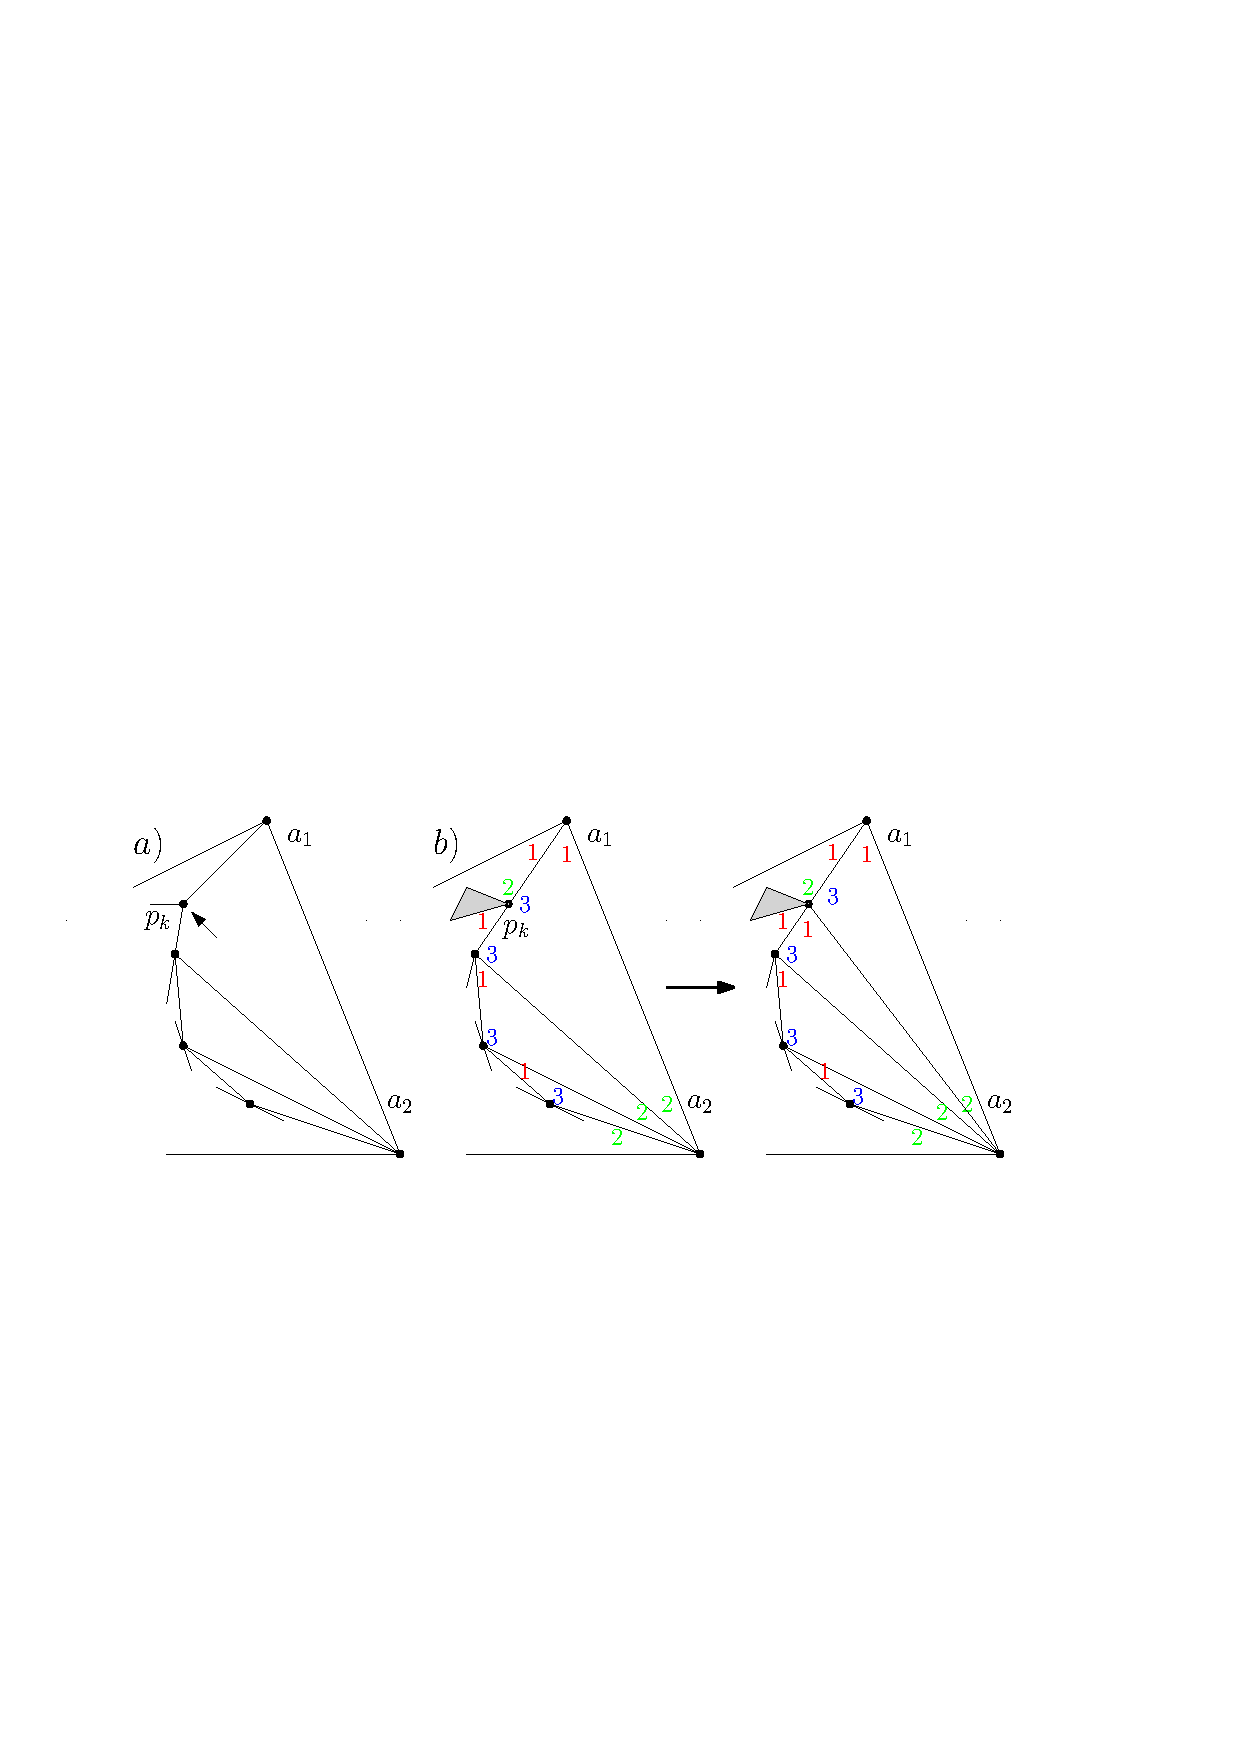
\includegraphics[width=1\textwidth]{lem6_3.pdf}
    	\caption{Ein Schnyder Labeling von $G_k$, erstellt aus einem Labeling von $G'$. }
    	\label{pic_lem6_3}
\end{figure}

Das Schnyder Labeling $\sigma'$ ist eindeutig für Gebiete mit $a_1$ oder $a_2$ als Ecken und einer geflippten Kante auf dem Rand (siehe Abbildung \ref{pic_lem6_3} b). In einem ersten Schritt müssen wir $(a_2,p_k)$ wieder einfügen und $\sigma'$ zu $\sigma_k$ erweitern (wie in Abbildung \ref{pic_lem6_3} b zu sehen ist).

Die Flips wurden entlang $q,p_1,\ldots,p_k$ durchgeführt und nach unserer Annahme haben die Knoten $p_1,\ldots,p_{k-1}$ von $\phi'$ zugewiesene Winkel in $G'$. Sei $p_0$=$q$. Zwei Knoten $p_{i-1}$ und $p_i$, mit $i \in \{1,\ldots,k\}$ in dieser Folge sind nicht zwangsläufig benachbart, aber sie sind die Ecken des (dreieckigen) Gebietes $a_2,p_{i-1},p_{i}$ und alle Knoten auf dem Rand zwischen $p_{i-1}$ und $p_{i}$ sind diesem Gebiet zugewiesen (siehe Abbildung \ref{pic_lem6_4} a). Wir führen nun Schritt für Schritt, beginnend mit $i=k$, einen \textit{Rückwärts-Flip} durch. Hierfür entfernen wir die Kante $(p_{i},a_2)$ und setzen die Kante $(p_{i},a_1)$ wieder ein. Merke, dass $p_{i}$ vor dem Schritt $i$ einen zusätzlichen Nachbarn in $G_{i}$ (im Verhältnis zu $G$) hat und somit gilt $\text{deg}(p_{i}) \geq 4$, weil $G$ intern-3-zusammenhängend ist. Wir benennen zwei der Winkel um den Knoten $p_i$. Sei $\alpha_{i}$ der gegen den Uhrzeigersinn auf die Kante $(p_i,a_1)$ folgende Winkel und $\beta_{i}$ der im Uhrzeigersinn auf die Kante zu $(p_i,p_{i-1})$ folgende Winkel an $p_{i}$ (vergleiche Abbildung \ref{pic_lem6_4} a). Dann handelt es sich bei diesen Winkeln, wegen $\text{deg}(p_i) \geq 4$, nicht um denselben. Bei jedem Schritt des Rückwärts-Flippens wird nun die folgende Invariante eingehalten.

\begin{invariant}
Vor dem Schritt $i$ hat der Knoten $p_i$ die Label 2,3,1,1 im Uhrzeigersinn beginnend mit den Winkel $\alpha_i$ und endend mit $\beta_i$ (siehe Abbildung \ref{pic_lem6_4} a). Zusätzlich bilden das Schnyder Labeling $\sigma'_i$ und das FAA $\phi'_i$ ein Ecken kompatibles Paar auf $G'_i$.
\end{invariant}

Beginnen wir mit $G'$. Hier sind die in Abbildung \ref{pic_lem6_3} b) gewählten Label der Winkel um $p_k$ die einzig mögliche Wahl. Genauso verhält es sich nach dem Einfügen der Kante $(a_2,p_k)$. Wir erhalten den Graphen $G'_{k}$, das Schnyder Labeling $\sigma'_{k}$ und das FAA $\phi'_{k}$, wobei $\sigma'_{k}$ und $\phi'_{k}$ ein Ecken kompatibles Paar bilden. Somit gilt die Invariante vor dem ersten Schritt.

Die Invariante gelte vor Schritt $i$. In Schritt $i$ entfernen wir die Kante $(a_2,p_i)$ und fügen die Kante $(a_1,p_{i-1})$ wieder in den Graphen ein. Vor dem Rückwärts-Flip, erfüllen die Label um $p_i$ die Invariante und $\sigma'_{i}$ und $\phi'_{i}$ sind ein Ecken kompatibles Paar. Die folgende Argumentation basiert auf Lemma \ref{lem_sl}, das besagt, dass alle drei Label im Uhrzeigersinn an jeder Kante vorkommen, und der Ecken Kompatibilität von $\sigma'_{i}$ und $\phi'_{i}$. Die Winkel an $p_{i-1}$ links und rechts der Kante zu $p_i$ haben die Label 2 und 3 (siehe Abbildung \ref{pic_lem6_4} b). Der Winkel zwischen $p_i$ und $a_2$ kann nur Label 3 haben, da er an einer Kante zu $a_2$ liegt, an deren anderen Ende somit nur Label 2 vorkommt. Der andere Winkel muss Label 2 haben, da er entweder an einer Kante mit zwei 3ern auf der anderen Seite liegt (vergleiche Abbildung \ref{pic_lem6_4} a) oder er an der Kante $(p_i,p_{i-1})$ liegt, welche $p_i$ nur Label 1 hat(vergleiche Abbildung \ref{pic_lem6_4} b). 

\begin{figure}
	\centering
	  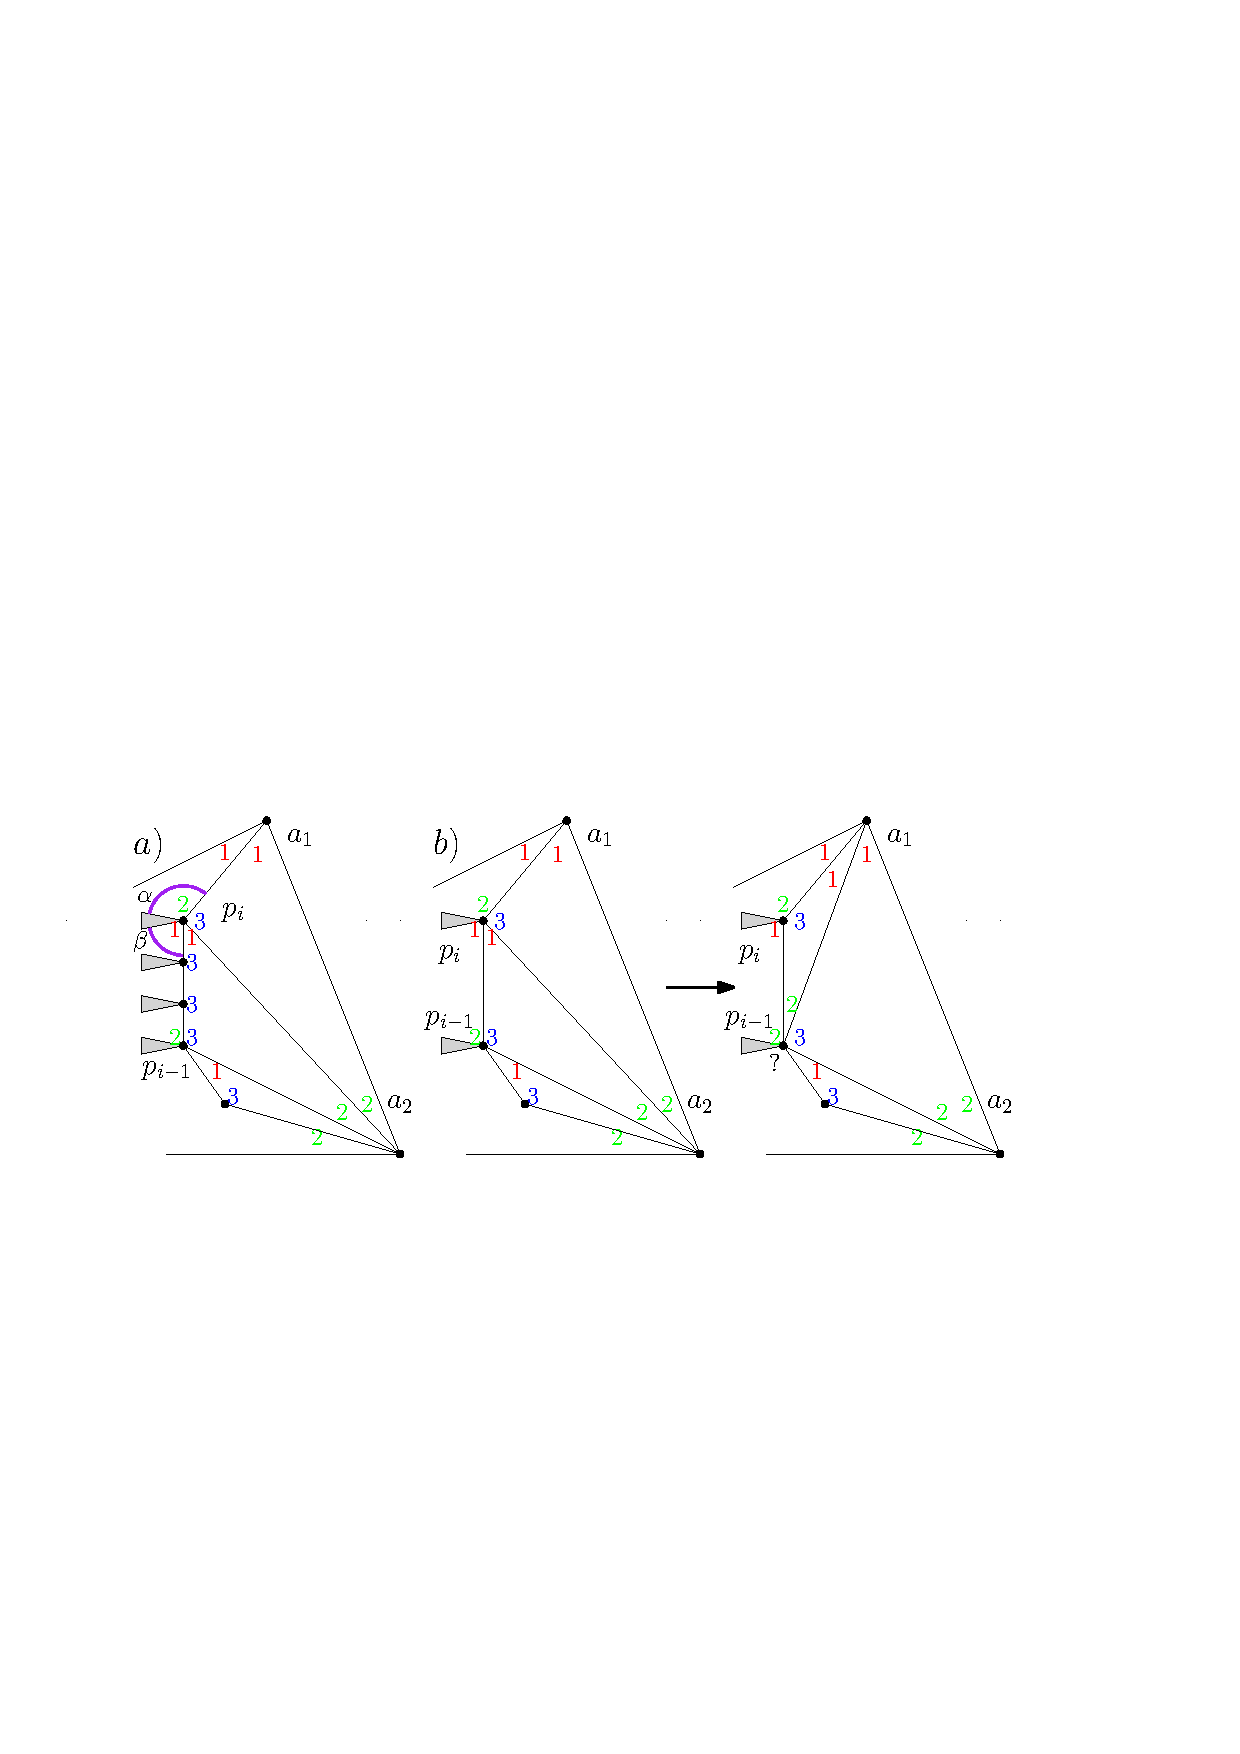
\includegraphics[width=1\textwidth]{lem6_4.pdf}
    	\caption{a) Schnyder Labeling zwischen $p_{i-1}$ und $p_{i}$ mit den Winkeln $\alpha$ und $\beta$ in violett. b) Änderung des Labelings beim Rückwärts-Flippen.}
    	\label{pic_lem6_4}
\end{figure}

Führen wir den \textit{Rückwärts-Flip} durch. Wir löschen also die Kante $(a_2,p_i)$ und fügen die Kante $(a_1,p_{i-1})$ ein, wie in Abbildung \ref{pic_lem6_4} b). Für fast alle Winkel folgt die Wahl des Labels eindeutig, da $\sigma'_{i-1}$ ein Schnyder Labeling sein muss. Um die Invariante zu erfüllen, müssen wir zeigen, dass wir dem mit einem Fragezeichen markierten Winkel in Abbildung \ref{pic_lem6_4} b) Label 1 geben können. Wenn er dieses Label schon vor dem Schritt hatte, ändert sich nichts und wir sind fertig. Angenommen, er hatte nicht Label 1. Da es sich um ein Schnyder Labeling handelt, ist die einzig andere Möglichkeit Label 2. Es muss sich bei diesem Winkel um den an $p_{i-1}$ zugewiesenen handeln. Dies folgt aus der Ecken Kompatibilität, da ein zugewiesener Winkel und seine beiden Nachbarn um einen Knoten nicht alle die gleichen Label haben können (siehe Abbildung \ref{pic_lem6_5} a), sonst würde es zu einem Widerspruch kommen. Es existieren mindestens zwei weitere Winkel an $p_{i-1}$ mit Label 2 (also insgesamt mindestens drei). Somit würde der Fall aus Abbildung \ref{pic_lem6_5} a) eintreten und ein angrenzendes Gebiet hätte keine Ecke mit Label 2. Der Winkel mit dem Fragezeichen muss somit zugewiesen sein.

\begin{figure}[h]
	\centering
	  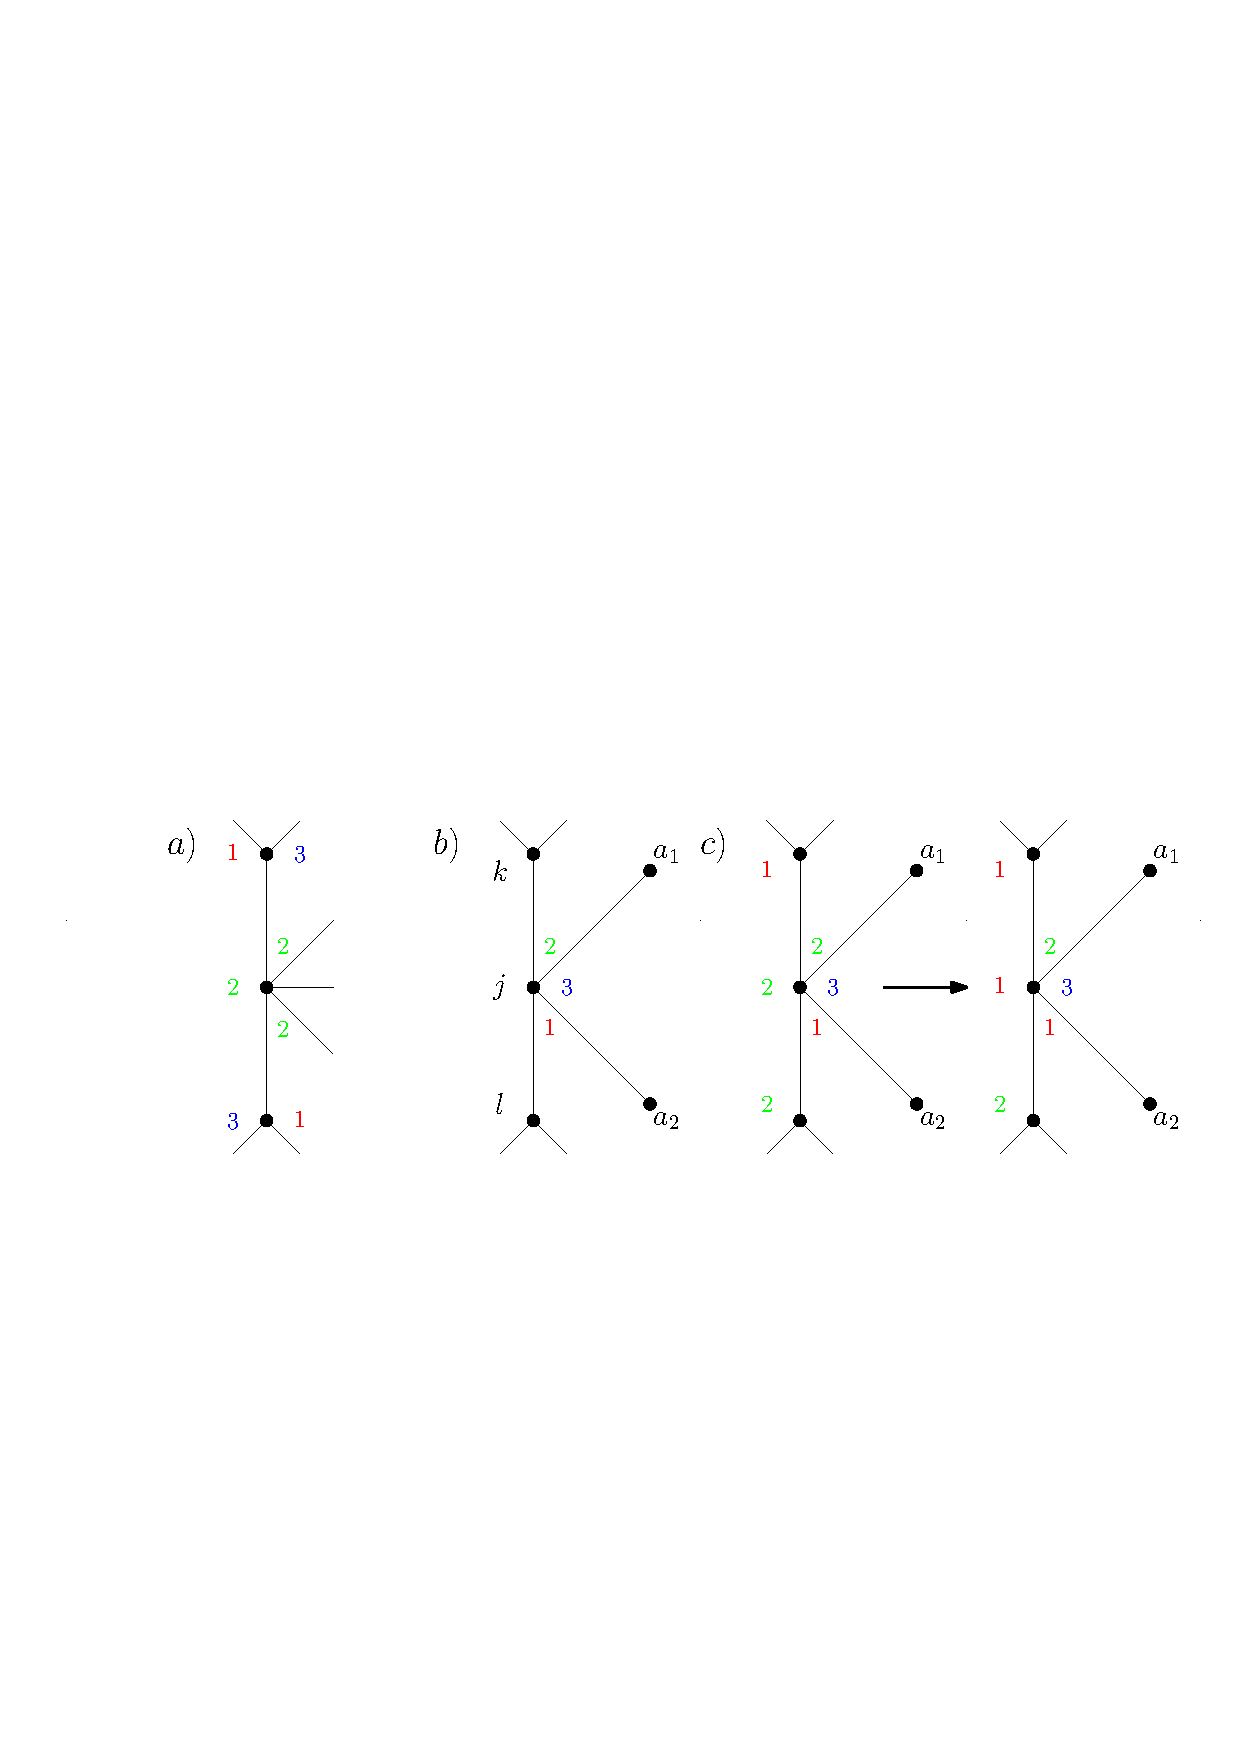
\includegraphics[width=0.9\textwidth]{lem6_5.pdf}
    	\caption{a) Das Gebiet links kann keine Ecke mit Label 1 haben. b) Eine freie Wahl von Winkel in einem Schnyder Labeling. c) Nach der Änderung von Label 2 zu Label 1 am zugewiesenen Knoten liegt weiterhin ein Ecken kompatibles Paar vor.}
    	\label{pic_lem6_5}
\end{figure}

Betrachte Abbildung \ref{pic_lem6_5} b). Wenn wir $j$=2 setzen, dann folgen sofort die Label in c). $k$=1 folgt aus der Kanten Regel, weil die Kante and $p_{i-1}$ auf beiden Seiten Label 2 hat, und $l$=2, weil sonst das Gebiet auf der linken Seite keine Ecke mit Label 2 haben könnte. Wir können nun Label $j$=1 setzen, ohne andere Label zu verändern. Wir erhalten ein Schnyder Labeling $\sigma'_{i-1}$ (siehe Abbildung \ref{pic_lem6_5} c), das Ecken kompatibel mit dem induzierten FAA $\phi'_{i-1}$ ist, da wir nur das Label eines zugewiesen Winkels verändert haben.

Wir haben also Schritt $i$ durchgeführt und die Invariante hat Bestand. Per Induktion erhalten wir ein Ecken kompatibles Paar aus einem Schnyder Labeling $\sigma'_0$ und einem FAA $\phi'_0$ von $G$. Somit kann $G$ kein Gegenbeispiel sein. Es folgt die Rückrichtung des Theorems.
\end{proof}

Wir haben nun alle nötigen Hilfsmittel erarbeitet, um das folgende, weiter oben schon aufgeführte Theorem zu beweisen.

\begin{reptheorem}{theo_ccc}
Sei G ein ebener, intern-3-zusammenhängender Graph mit den Aufhängungen $\{a_1,a_2,a_3\}$. G besitzt eine SLTR, genau dann, wenn ein Ecken kompatibles Paar $(\sigma,\phi)$ aus einem Schnyder Labeling $\sigma$ und einem FAA $\phi$ existiert.
\end{reptheorem}

\begin{proof}[Beweis von Theorem \ref{theo_ccc}]
Sei G ein ebener, intern-3-zusammenhängender Graph mit den Aufhängungen $\{a_1,a_2,a_3\}$. Angenommen $G$ besitzt ein Ecken kompatibles Paar $(\sigma,\phi)$ aus einem Schnyder Labeling $\sigma$ und einem FAA $\phi$. Nach Lemma \ref{lem1} existiert dann eine SLTR von $G$. 

Angenommen $G$ besitzt eine SLTR, dann existert nach Lemma \ref{lem6} ein Schnyder Labeling, das Ecken kompatibel mit dem von der SLTR induzierten FAA ist.
\end{proof}

Theorem \ref{theo_ccc} liefert noch keinen direkten Weg, um für einen Graphen die Frage zu beantworten, ob er eine SLTR zulässt. Im nächsten Kapitel werden wir uns aber mit einem Algorithmus befassen, der den Zusammenhang aus Theorem \ref{theo_ccc} nutzt, um für einen Graphen ein Gutes-FAA zu erkennen, falls er eine SLTR zulässt.

\begin{figure}[h]
	\centering
  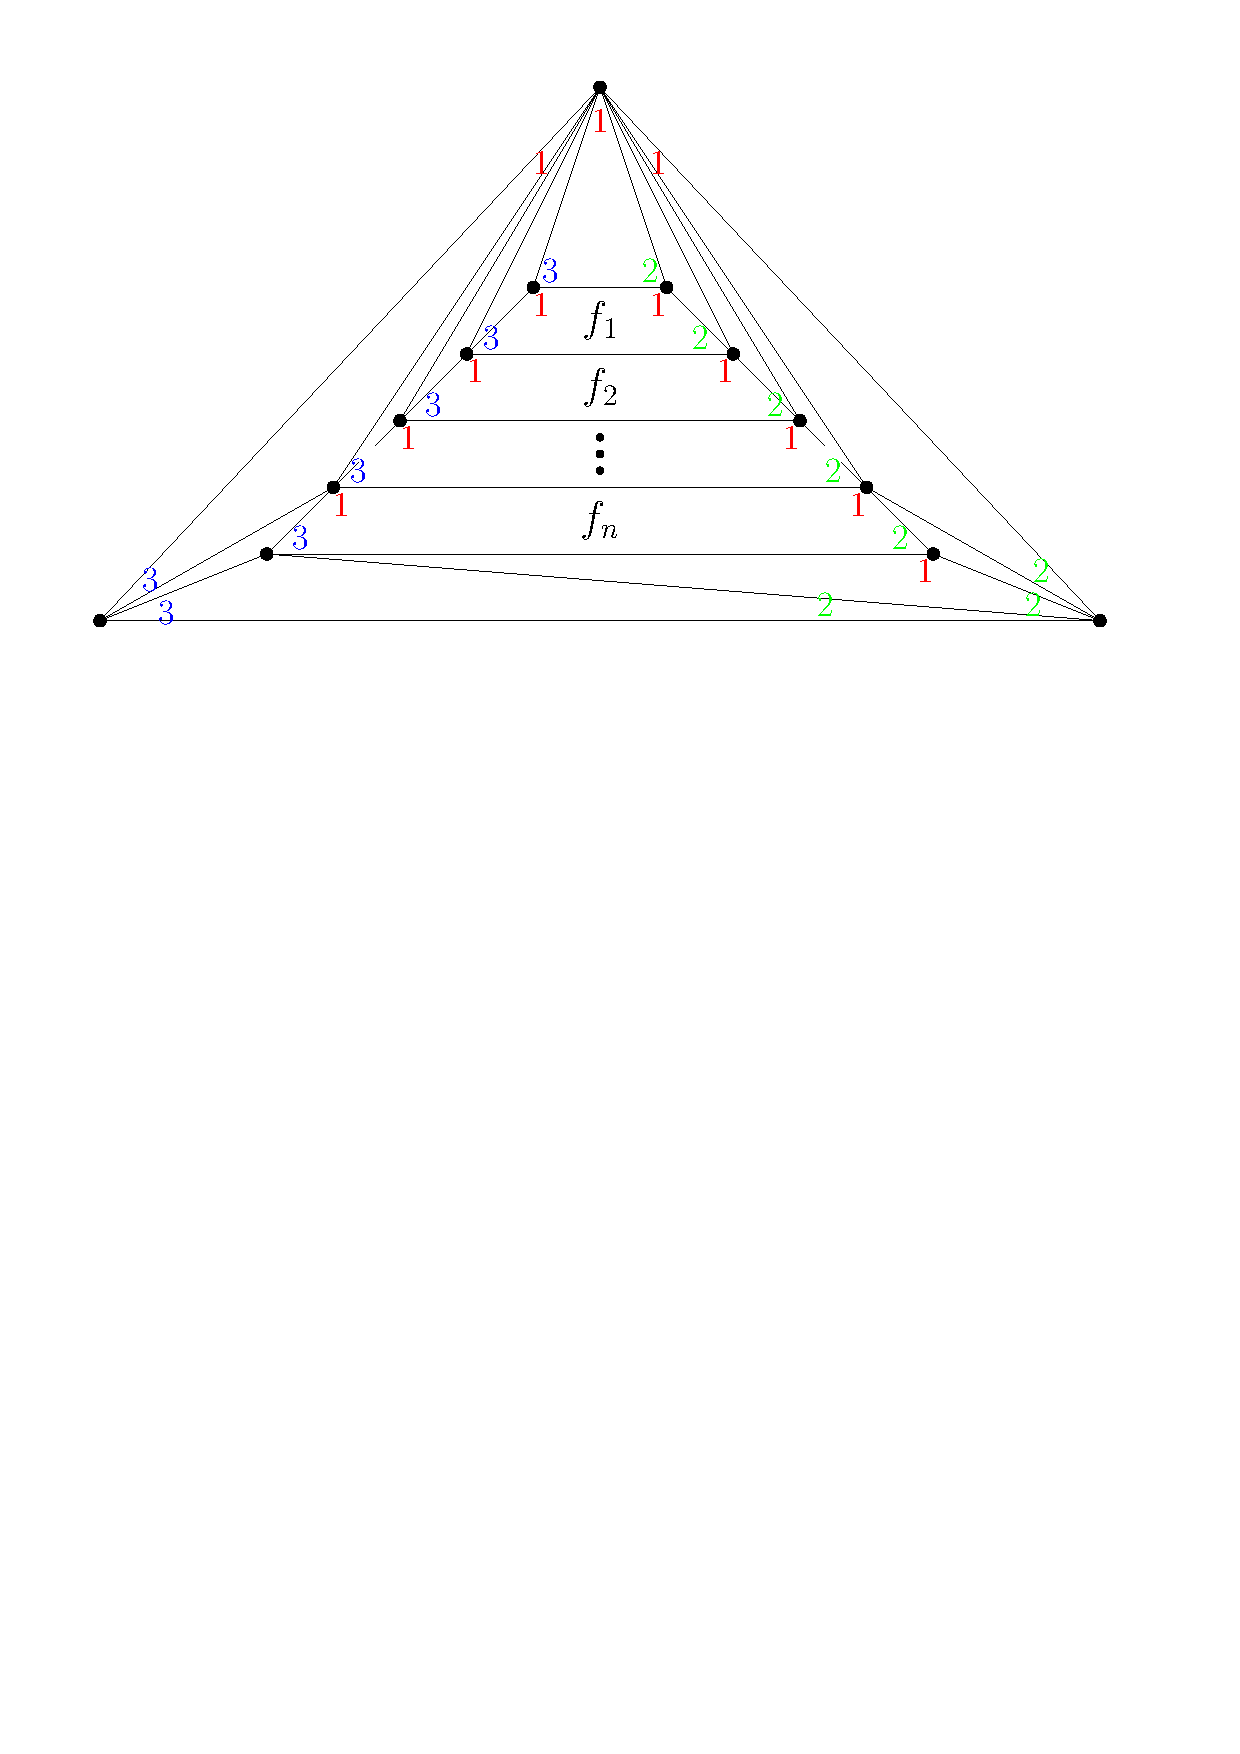
\includegraphics[width=0.7\textwidth]{exp_many_sltr.pdf}
  \caption{Ein Graph mit exponentiell vielen SLTRs.}
  \label{exp_many_sltr}
\end{figure}

\begin{example}
Wir können Beispiel \ref{bsp_exp_faa} leicht anpassen, um mit Theorem \ref{theo_ccc} zeigen, dass es Graphen mit exponentiell vielen SLTRs gibt. Zu dem Schnyder Labeling $\sigma$ des Graphen $G$ auf $2n+3$ Knoten, der in Abbildung \ref{exp_many_sltr} zu sehen ist, existieren $2^n$ viele FAAs, um ein Ecken kompatibles Paar zu bilden. Wir können in jedem Viereck einen der beiden oberen Knoten zuweisen, unabhängig davon, welche Knoten in den restlichen Vierecken zugewiesen sind, um ein FAA $\phi$ zu konstruieren. Somit haben die inneren Gebiete jeweils eine Ecke (bezüglich $\phi$) mit jedem Label aus $\sigma$.
\end{example}




